% Contents from body/page-370.tex.
\BookMark{0}{V  Surfaces}{p-370}
\ChapterSheet{370}{356}{}{%
\vspace*{22pt}
\noindent{\large\bfseries V}\par\vspace{3pt}
\hrule
\vspace{6pt}
\noindent{\Large\bfseries Surfaces}\par
\vspace{161pt}
\noindent In this chapter we give an introduction to the study of algebraic surfaces. This includes the basic facts about the geometry on a surface, and about birational transformations of surfaces. Also we treat two special classes of surfaces, the ruled surfaces, and the nonsingular cubic surfaces in $\Proj^3$, both to illustrate the general theory, and as a first step in the more detailed study of various types of surfaces.

This chapter should be adequate preparation for reading some more advanced works, such as Mumford \Goto{bib-mumford-2}{[2]}, Zariski \Goto{bib-zariski-5}{[5]}, Shafarevich \Goto{bib-482-7}{[1]}, Bombieri and Husemoller \Goto{bib-bombieri-husemoller-1}{[1]}. We have mentioned the classification of surfaces only very briefly in \Goto{sec-V-6}{\S6}, since it is adequately treated elsewhere.

Sections \Goto{sec-V-1}{1}, \Goto{sec-V-3}{3} and \Goto{sec-V-5}{5} are general. Here we develop intersection theory on a surface and prove the Riemann--Roch theorem. As applications we give the Hodge index theorem and the Nakai--Moishezon criterion for an ample divisor. In \Goto{sec-V-3}{\S3} we study the behavior of a surface and the curves on it under a single monoidal transformation, which is blowing up a point. Then in \Goto{sec-V-5}{\S5} we prove the theorem of factorization of a birational morphism into monoidal transformations, and prove Castelnuovo's criterion for contracting an exceptional curve of the first kind.

In \Goto{sec-V-2}{\S2} we discuss ruled surfaces. Here the theory of curves gives a good handle on the ruled surfaces, because many properties of the surface are closely related to the study of certain linear systems on the base curve. Also there is a close connection between ruled surfaces over a curve $C$ and locally free sheaves of rank $2$ on $C$, so as a byproduct, we get some information about the classification of these locally free sheaves on a curve.

In \Goto{sec-V-4}{\S4}, we study the nonsingular cubic surfaces in $\Proj^3$, and the famous $27$ lines which lie on those surfaces. By representing the surface as a $\Proj^2$ with $6$ points blown up, the study of linear systems on the cubic surface is reduced
}
% Contents from body/page-371.tex.
\BookMark{1}{5.1  Geometry on a Surface}{sec-V-1}
\ChapterSheet{371}{357}{1\quad Geometry on a Surface}{%
to the study of certain linear system of plane curves with assigned base points. This is a very classical subject, about which whole books have been written, and which we rewrite here in modern language.

\vspace{16pt}
\noindent\hypertarget{sec-V-1}{}{\large\bfseries 1\quad Geometry on a Surface}\par\nobreak\vspace{9pt}
\noindent We begin our study of surfaces with the internal geometry of a surface. A divisor on a surface is a sum of curves, so (in the absence of a projective embedding) it does not make sense to talk about the degree of a divisor, as in the case of curves. However, we can talk about the intersection of two divisors on a surface, and this gives rise to intersection theory. The Riemann--Roch theorem for surfaces gives a connection between the dimension of a complete linear system $|D|$, which is essentially a cohomological invariant, and certain intersection numbers on the surface. As in the case of curves, the Riemann--Roch theorem is basic to all further work with surfaces, especially questions of classification.

Throughout this chapter, a \emph{surface} will mean a nonsingular projective surface over an algebraically closed field $k$. It is true that any complete nonsingular surface is projective (cf.\ II, \Goto{result-II-4.10.2}{4.10.2}), but since we will not prove that, we assume that our surfaces are projective. A \emph{curve} on a surface will mean any effective divisor on the surface. In particular, it may be singular, reducible or even have multiple components. A \emph{point} will mean a closed point, unless otherwise specified.

\medskip
Let $X$ be a surface. We wish to define the intersection number $C\cdot D$ for any two divisors $C,D$ on $X$ in such a way as to generalize the intersection multiplicity defined in (I, Ex.~\Goto{ex-I-5.4}{5.4}) and (I, \Goto{sec-I-7}{\S7}). If $C$ and $D$ are curves on $X$, and if $P\in C\cap D$ is a point of intersection of $C$ and $D$, we say that $C$ and $D$ meet \emph{transversally} at $P$ if the local equations $f,g$ of $C,D$ at $P$ generate the maximal ideal $\mathfrak m_P$ of $\mathcal O_{P,X}$. This implies, by the way, that $C$ and $D$ are each nonsingular at $P$, because $f$ will generate the maximal ideal of $P$ in $\mathcal O_{P,D}=\mathcal O_{P,X}/(g)$, and vice versa.

If $C$ and $D$ are two nonsingular curves, which meet transversally at a finite number of points $P_1,\ldots,P_r$, then it is clear that the intersection number $C\cdot D$ should be $r$. So we take this as our starting point, together with some natural properties the intersection pairing should have, to define our intersection theory. We denote by $\operatorname{Div}X$ the group of all divisors on $X$, and by $\operatorname{Pic}X$ the group of invertible sheaves up to isomorphism, which is isomorphic to the group of divisors modulo linear equivalence (II, \Goto{sec-II-6}{\S6}).

\medskip
\noindent\hypertarget{result-V-1.1}{}\textbf{Theorem 1.1.} \emph{There is a unique pairing $\operatorname{Div}X\times\operatorname{Div}X\to\mathbf Z$, denoted by $C\cdot D$ for any two divisors $C,D$, such that}
\par{\itshape\leftskip=13pt
\noindent\hypertarget{result-V-1.1-1}{}(1) if $C$ and $D$ are nonsingular curves meeting transversally, then $C\cdot D=\#(C\cap D)$, the number of points of $C\cap D$,\par}
}
% Contents from body/page-372.tex.
\ChapterSheet{372}{358}{\Goto{p-370}{V\quad Surfaces}}{%
{\itshape\leftskip=13pt
\noindent\hypertarget{result-V-1.1-2}{}(2) it is symmetric: $C\cdot D=D\cdot C$,

\noindent\hypertarget{result-V-1.1-3}{}(3) it is additive: $(C_1+C_2)\cdot D=C_1\cdot D+C_2\cdot D$, and

\noindent\hypertarget{result-V-1.1-4}{}(4) it depends only on the linear equivalence classes: if $C_1\sim C_2$ then $C_1\cdot D=C_2\cdot D$.\par}

\medskip
Before giving the proof, we need some auxiliary results. Our main tool is Bertini's theorem, which we will use to express any divisor as a difference of nonsingular curves, up to linear equivalence.

\medskip
\noindent\hypertarget{result-V-1.2}{}\textbf{Lemma 1.2.} \emph{Let $C_1,\ldots,C_r$ be irreducible curves on the surface $X$, and let $D$ be a very ample divisor. Then almost all curves $D'$ in the complete linear system $|D|$ are irreducible, nonsingular, and meet each of the $C_i$ transversally.}

\smallskip
\noindent\textsc{Proof.} We embed $X$ in a projective space $\Proj^n$ using the very ample divisor $D$. Then we apply Bertini's theorem (II, \Goto{result-II-8.18}{8.18}) and (III, \Goto{result-III-7.9.1}{7.9.1}) simultaneously to $X$ and to the curves $C_1,\ldots,C_r$. We conclude that most $D'\in|D|$ are irreducible nonsingular curves in $X$, and that the intersections \EditionText{$C_i\cap D'$} are nonsingular, i.e., points with multiplicity one, which means that the $C_i$ and $D'$ meet transversally. Since we did not assume the $C_i$ were nonsingular, we need to use (II, \Goto{result-II-8.18.1}{8.18.1}).

\medskip
\noindent\hypertarget{result-V-1.3}{}\textbf{Lemma 1.3.} \emph{Let $C$ be an irreducible nonsingular curve on $X$, and let $D$ be any curve meeting $C$ transversally. Then}
\[
\#(C\cap D)=\deg_C(\mathcal L(D)\otimes\mathcal O_C).
\]

\smallskip
\noindent\textsc{Proof.} Here, of course, $\mathcal L(D)$ is the invertible sheaf on $X$ corresponding to $D$ (II, \Goto{sec-II-7}{\S7}), and $\deg_C$ denotes the degree of the invertible sheaf $\mathcal L(D)\otimes\mathcal O_C$ on $C$ (IV, \Goto{sec-IV-1}{\S1}). We use the fact (II, \Goto{result-II-6.18}{6.18}) that $\mathcal L(-D)$ is the ideal sheaf of $D$ on $X$. Therefore, tensoring with $\mathcal O_C$, we have an exact sequence
\[
0\to\mathcal L(-D)\otimes\mathcal O_C\to\mathcal O_C\to\mathcal O_{C\cap D}\to0
\]
where now $C\cap D$ denotes the scheme-theoretic intersection. Thus $\mathcal L(D)\otimes\mathcal O_C$ is the invertible sheaf on $C$ corresponding to the divisor $C\cap D$. Since the intersection is transversal, the degree of the divisor $C\cap D$ is just the number of points $\#(C\cap D)$.

\medskip
\noindent\textsc{Proof of} \Goto{result-V-1.1}{(1.1)}. First we show the uniqueness. Fix an ample divisor $H$ on $X$. Given any two divisors $C,D$ on $X$, we can find an integer $n>0$ such that $C+nH$, $D+nH$, and $nH$ are all very ample. Indeed, we first choose $k>0$ such that $\mathcal L(C+kH)$, $\mathcal L(D+kH)$ and $\mathcal L(kH)$ are all generated by global sections. This is possible by definition of ampleness (II, \Goto{sec-II-7}{\S7}). Then we choose $l>0$ so that $lH$ is very ample (II, \Goto{result-II-7.6}{7.6}). Taking $n=k+l$, it follows that $C+nH$, $D+nH$, and $nH$ are all very ample (II, Ex.~\Goto{ex-II-7.5}{7.5}).
}
% Contents from body/page-373.tex.
\ChapterSheet{373}{359}{\Goto{sec-V-1}{1\quad Geometry on a Surface}}{%
\indent Now using \Goto{result-V-1.2}{(1.2)}, choose nonsingular curves
\[
\begin{aligned}
&C'\in|C+nH|\\
&D'\in|D+nH|,\quad\text{transversal to }C'\\
&E'\in|nH|,\quad\text{transversal to }D'\\
&F'\in|nH|,\quad\text{transversal to }C'\text{ and }E'.
\end{aligned}
\]
Then $C\sim C'-E'$ and $D\sim D'-F'$, so by the properties \Goto{result-V-1.1-1}{(1)}--\Goto{result-V-1.1-4}{(4)} of the theorem, we have
\[
C\cdot D=\#(C'\cap D')-\#(C'\cap F')-\#(E'\cap D')+\#(E'\cap F').
\]
This shows that the intersection number of any two divisors is determined by \Goto{result-V-1.1-1}{(1)}--\Goto{result-V-1.1-4}{(4)}, so the intersection pairing is unique.

For the existence, we use the same method, and check that everything is well-defined. To simplify matters, we proceed in two steps. Let $\mathfrak P\subseteq\operatorname{Div}X$ be the set of very ample divisors. Then $\mathfrak P$ is a cone, in the sense that the sum of two very ample divisors is again very ample. For $C,D\in\mathfrak P$, we define the intersection number $C\cdot D$ as follows: by \Goto{result-V-1.2}{(1.2)} choose $C'\in|C|$ nonsingular, and choose $D'\in|D|$ nonsingular and transversal to $C'$. Define $C\cdot D=\#(C'\cap D')$.

To show this is well-defined, first fix $C'$, and let $D''\in|D|$ be another nonsingular curve, transversal to $C'$. Then by \Goto{result-V-1.3}{(1.3)}, we have
\[
\#(C'\cap D')=\deg\mathcal L(D')\otimes\mathcal O_{C'},
\]
and ditto for $D''$. But $D'\sim D''$, so $\mathcal L(D')\cong\mathcal L(D'')$, so these two numbers are the same. Thus our definition is independent of $D'$. Now suppose $C''\in|C|$ is another nonsingular curve. By the previous step, we may assume $D'$ is transversal to both $C'$ and $C''$. Then by the same argument, restricting to the curve $D'$, we see that $\#(C'\cap D')=\#(C''\cap D')$.

So now we have a well-defined pairing $\mathfrak P\times\mathfrak P\to\mathbf Z$, which is clearly symmetric, and by definition it depends only on the linear equivalence classes of the divisors. It also follows from \Goto{result-V-1.3}{(1.3)} that it is additive, since $\mathcal L(D_1+D_2)\cong\mathcal L(D_1)\otimes\mathcal L(D_2)$, and the degree is additive on a curve. Finally, this pairing on $\mathfrak P\times\mathfrak P$ satisfies condition \Goto{result-V-1.1-1}{(1)} by construction.

To define the intersection pairing on all of $\operatorname{Div}X$, let $C$ and $D$ be any two divisors. Then, as above, we can write $C\sim C'-E'$ and $D\sim D'-F'$ where $C',D',E',F'$ are all in $\mathfrak P$. So we define
\[
C\cdot D=C'\cdot D'-C'\cdot F'-E'\cdot D'+E'\cdot F'.
\]
If, for example, we used another expression $C\sim C''-E''$ with $C'',E''$ also very ample, then
\[
C'+E''\sim C''+E',
\]
so by what we have shown for the pairing in $\mathfrak P$, we have
\[
C'\cdot D'+E''\cdot D'=C''\cdot D'+E'\cdot D'
\]
}
% Contents from body/page-374.tex.
\ChapterSheet[\EditionText{10.52}]{374}{360}{\Goto{p-370}{V\quad Surfaces}}{%
and ditto for $F'$ in place of $D'$. Thus the resulting two expressions for $C\cdot D$ are the same. This shows that the intersection pairing $C\cdot D$ is well-defined on all of $\operatorname{Div}X$.

It satisfies \Goto{result-V-1.1-2}{(2)}, \Goto{result-V-1.1-3}{(3)}, \Goto{result-V-1.1-4}{(4)} by construction and by the corresponding properties on $\mathfrak P$. The condition \Goto{result-V-1.1-1}{(1)} follows using \Goto{result-V-1.3}{(1.3)} once more.\hfill q.e.d.

\medskip
Now that we have defined the intersection pairing, it is useful to have a way of calculating it without having to move the curves. If $C$ and $D$ are curves with no common irreducible component, and if $P\in C\cap D$, then we define the \emph{intersection multiplicity} $(C\cdot D)_P$ of $C$ and $D$ at $P$ to be the length of $\mathcal O_{P,X}/(f,g)$, where $f,g$ are local equations of $C,D$ at $P$ (I, Ex.~\Goto{ex-I-5.4}{5.4}). Here \emph{length} is the same as the dimension of a $k$-vector space.

\medskip
\noindent\hypertarget{result-V-1.4}{}\textbf{Proposition 1.4.} \emph{If $C$ and $D$ are curves on $X$ having no common irreducible component, then}
\[
C\cdot D=\sum_{P\in C\cap D}(C\cdot D)_P.
\]

\smallskip
\noindent\textsc{Proof.} As in the proof of \Goto{result-V-1.3}{(1.3)}, let $\mathcal L(D)$ be the invertible sheaf corresponding to $D$. Then we have an exact sequence
\[
0\to\mathcal L(-D)\otimes\mathcal O_C\to\mathcal O_C\to\mathcal O_{C\cap D}\to0
\]
where we consider $C\cap D$ as a scheme. Now the scheme $C\cap D$ has support at the points of $C\cap D$, and for any such $P$, its structure sheaf is the $k$-algebra $\mathcal O_{P,X}/(f,g)$. Therefore
\[
\dim_k H^0(X,\mathcal O_{C\cap D})=\sum_{P\in C\cap D}(C\cdot D)_P.
\]
On the other hand, we can calculate this $H^0$ from the cohomology sequence of the exact sequence above. We obtain
\[
\dim H^0(X,\mathcal O_{C\cap D})=\chi(\mathcal O_C)-\chi(\mathcal L(-D)\otimes\mathcal O_C),
\]
where, as usual, for any coherent sheaf $\mathcal F$,
\[
\chi(\mathcal F)=\sum(-1)^i\dim_k H^i(X,\mathcal F)
\]
is the Euler characteristic (III, Ex.~\Goto{ex-III-5.1}{5.1}).

This shows that the expression $\sum(C\cdot D)_P$ depends only on the linear equivalence class of $D$. By symmetry, it also depends only on the linear equivalence class of $C$.
\EditionText{Write $i(C,D)$ for this sum. It is additive under sums of effective divisors $D_1,D_2$ avoiding the components of $C$. Indeed, if their equations in $R=\mathcal O_{C,P}$ are $g_1,g_2$, then $g_2$ is a nonzerodivisor, since $C$ is Cohen--Macaulay and $D_2$ avoids its components. Thus
\[
0\to R/(g_1)\xrightarrow{\cdot g_2} R/(g_1g_2)\to R/(g_2)\to0.
\]
Choose $D',F'$ as in the proof of \Goto{result-V-1.1}{(1.1)}, avoiding the components of $C$. Since $D+F'\sim D'$, invariance and additivity give $i(C,D)=i(C,D')-i(C,F')$. Similarly replace $C$ by $C'-E'$, with $C',E'$ transversal to $D',F'$. The four sums count distinct intersection points, so their alternating sum is the intersection number defined in \Goto{result-V-1.1}{(1.1)}.}

\smallskip
\noindent\hypertarget{result-V-1.4.1}{}\textbf{Example 1.4.1.} If $D$ is any divisor on the surface $X$, we can define the \emph{self-intersection} number $D\cdot D$, usually denoted by $D^2$. Even if $C$ is a nonsingular curve on $X$, the self-intersection $C^2$ cannot be calculated by the direct method
}
% Contents from body/page-375.tex.
\ChapterSheet{375}{361}{\Goto{sec-V-1}{1\quad Geometry on a Surface}}{%
of \Goto{result-V-1.4}{(1.4)}. We must use linear equivalence. However, by \Goto{result-V-1.3}{(1.3)}, we see that $C^2=\deg_C(\mathcal L(C)\otimes\mathcal O_C)$. To reinterpret this, note that since the ideal sheaf $\mathcal I$ of $C$ on $X$ is $\mathcal L(-C)$ (II, \Goto{result-II-6.18}{6.18}), we have $\mathcal I/\mathcal I^2\cong\mathcal L(-C)\otimes\mathcal O_C$. Therefore its dual $\mathcal L(C)\otimes\mathcal O_C$ is isomorphic to the \emph{normal sheaf} $\mathcal N_{C/X}$, which is defined as $\mathcal H\!om(\mathcal I/\mathcal I^2,\mathcal O_C)$ (II, \Goto{sec-II-8}{\S8}). So we have $C^2=\deg_C\mathcal N_{C/X}$.

\medskip
\noindent\hypertarget{result-V-1.4.2}{}\textbf{Example 1.4.2.} Let $X=\Proj^2$. Then $\operatorname{Pic}X\cong\mathbf Z$, and we can take the class $h$ of a line as generator. Since any two lines are linearly equivalent, and since two distinct lines meet in one point, we have $h^2=1$. This determines the intersection pairing on $\Proj^2$, by linearity. Thus if $C,D$ are curves of degrees $n,m$ respectively, we have $C\sim nh$, $D\sim mh$ and so $C\cdot D=nm$. If $C$ and $D$ have no component in common this can be interpreted in terms of the local intersection multiplicities of \Goto{result-V-1.4}{(1.4)}, and we get a new proof of B\'ezout's theorem (I, \Goto{result-I-7.8}{7.8}).

\medskip
\noindent\hypertarget{result-V-1.4.3}{}\textbf{Example 1.4.3.} Let $X$ be the nonsingular quadric surface in $\Proj^3$. Then $\operatorname{Pic}X\cong\mathbf Z\oplus\mathbf Z$ (II, \Goto{result-II-6.6.1}{6.6.1}) and we can take as generators lines $l$ of type $(1,0)$ and $m$ of type $(0,1)$, one from each family. Then $l^2=0$, $m^2=0$, $l\cdot m=1$, because two lines in the same family are skew, and two lines of opposite families meet in a point. This determines the intersection pairing on $X$. So for example if $C$ has type $(a,b)$ and $D$ has type $(a',b')$, then $C\cdot D=ab'+a'b$.

\medskip
\noindent\hypertarget{result-V-1.4.4}{}\textbf{Example 1.4.4.} Using the self-intersection, we can define a new numerical invariant of a surface. Let $\Omega_{X/k}$ be the sheaf of differentials of $X/k$, and let $\omega_X=\bigwedge^2\Omega_{X/k}$ be the \emph{canonical sheaf}, as defined in (II, \Goto{sec-II-8}{\S8}). Any divisor $K$ in the linear equivalence class corresponding to $\omega_X$ is called a \emph{canonical divisor}. Then $K^2$, the self-intersection of the canonical divisor, is a number depending only on $X$. For example, if $X=\Proj^2$, $K=-3h$, so $K^2=9$. If $X$ is the quadric surface \Goto{result-V-1.4.3}{(1.4.3)}, then $K$ has type $(-2,-2)$ (II, Ex.~\Goto{ex-II-8.4}{8.4}), so $K^2=8$.

\medskip
\noindent\hypertarget{result-V-1.5}{}\textbf{Proposition 1.5} (Adjunction Formula). \emph{If $C$ is a \EditionText{nonsingular irreducible curve} of genus $g$ on the surface $X$, and if $K$ is the canonical divisor on $X$, then}
\[
2g-2=C\cdot(C+K).
\]

\smallskip
\noindent\textsc{Proof.} According to (II, \Goto{result-II-8.20}{8.20}) we have $\omega_C\cong\omega_X\otimes\mathcal L(C)\otimes\mathcal O_C$. The degree of $\omega_C$ is $2g-2$ (IV, \Goto{result-IV-1.3.3}{1.3.3}). On the other hand, by \Goto{result-V-1.3}{(1.3)} we have
\[
\deg_C(\omega_X\otimes\mathcal L(C)\otimes\mathcal O_C)=C\cdot(C+K).
\]

\medskip
\noindent\hypertarget{result-V-1.5.1}{}\textbf{Example 1.5.1.} This gives a quick method of computing the genus of a curve on a surface. For example, if $C$ is a \EditionText{nonsingular irreducible curve} of degree $d$ in $\Proj^2$, then
\[
2g-2=d(d-3)
\]
so $g=\tfrac12(d-1)(d-2)$. Cf. (II, Ex.~\Goto{ex-II-8.4}{8.4}).\EditionText{ For any nonzero effective divisor of degree $d$, the same formula computes $p_a(C)$ (Ex.~\Goto{ex-V-1.3}{1.3a}).}
}
% Contents from body/page-376.tex.
\ChapterSheet{376}{362}{\Goto{p-370}{V\quad Surfaces}}{%
\noindent\hypertarget{result-V-1.5.2}{}\textbf{Example 1.5.2.} If $C$ is a \EditionText{nonsingular irreducible curve} of type $(a,b)$ on the quadric surface, then $C+K$ has type $(a-2,b-2)$, so
\[
2g-2=a(b-2)+(a-2)b,
\]
so $g=ab-a-b+1$. Cf. (III, Ex.~\Goto{ex-III-5.6}{5.6}).\EditionText{ For any nonzero effective divisor of type $(a,b)$, the same formula computes $p_a(C)$ (Ex.~\Goto{ex-V-1.3}{1.3a}).}

\medskip
Now we come to the Riemann--Roch theorem. For any divisor $D$ on the surface $X$, we let $l(D)=\dim_k H^0(X,\mathcal L(D))$. Thus $l(D)=\dim|D|+1$, where $|D|$ is the complete linear system of $D$. We define the \emph{superabundance} $s(D)$ to be $\dim H^1(X,\mathcal L(D))$. The reason for this terminology is that before the invention of cohomology, the Riemann--Roch formula was written only with $l(D)$ and $l(K-D)$, and the superabundance was the amount by which it failed to hold. Recall also that the \emph{arithmetic genus} $p_a$ of $X$ is defined by $p_a=\chi(\mathcal O_X)-1$ (III, Ex.~\Goto{ex-III-5.3}{5.3}).

\medskip
\noindent\hypertarget{result-V-1.6}{}\textbf{Theorem 1.6} (Riemann--Roch). \emph{If $D$ is any divisor on the surface $X$, then}
\[
l(D)-s(D)+l(K-D)=\tfrac12D\cdot(D-K)+1+p_a.
\]

\smallskip
\noindent\textsc{Proof.} By Serre duality (III, \Goto{result-III-7.7}{7.7}) we have
\[
l(K-D)=\dim H^0(X,\mathcal L(D)^\vee\otimes\omega_X)=\dim H^2(X,\mathcal L(D)).
\]
Thus the left-hand side is just the Euler characteristic, so we have to show for any $D$ that
\[
\chi(\mathcal L(D))=\tfrac12D\cdot(D-K)+1+p_a.
\]

Since both sides depend only on the linear equivalence class of $D$, as in \Goto{result-V-1.1}{(1.1)} we can write $D$ as the difference $C-E$ of two nonsingular curves. Now let us calculate. Since the ideal sheaves of $C,E$ are $\mathcal L(-C),\mathcal L(-E)$ respectively, we obtain exact sequences, tensoring with $\mathcal L(C)$,
\[
0\to\mathcal L(C-E)\to\mathcal L(C)\to\mathcal L(C)\otimes\mathcal O_E\to0
\]
and
\[
0\to\mathcal O_X\to\mathcal L(C)\to\mathcal L(C)\otimes\mathcal O_C\to0.
\]
Since $\chi$ is additive on short exact sequences (III, Ex.~\Goto{ex-III-5.1}{5.1}), we have
\[
\chi(\mathcal L(C-E))=\chi(\mathcal O_X)+\chi(\mathcal L(C)\otimes\mathcal O_C)-\chi(\mathcal L(C)\otimes\mathcal O_E).
\]
Now $\chi(\mathcal O_X)=1+p_a$ by definition of $p_a$. Using the Riemann--Roch theorem for the curves $C$ and $E$ (IV, \Goto{result-IV-1.3}{1.3}), and using \Goto{result-V-1.3}{(1.3)} to find the degree, we have
\[
\chi(\mathcal L(C)\otimes\mathcal O_C)=C^2+1-g_C
\]
and
\[
\chi(\mathcal L(C)\otimes\mathcal O_E)=C\cdot E+1-g_E.
\]
}
% Contents from body/page-377.tex.
\ChapterSheet{377}{363}{\Goto{sec-V-1}{1\quad Geometry on a Surface}}{%
Finally, we use \Goto{result-V-1.5}{(1.5)} to compute the genus of $C$ and $E$:
\[
g_C=\tfrac12 C\cdot(C+K)+1
\]
and
\[
g_E=\tfrac12 E\cdot(E+K)+1.
\]
Combining all these, we obtain
\[
\chi(\mathcal L(C-E))=\tfrac12(C-E)\cdot(C-E-K)+1+p_a
\]
as required.

\medskip
\noindent\hypertarget{result-V-1.6.1}{}\textbf{Remark 1.6.1.} There is another formula, which is sometimes considered to be part of the Riemann--Roch theorem, namely
\[
12(1+p_a)=K^2+c_2,
\]
where $c_2$ is the second Chern class of the tangent sheaf of $X$. This is a consequence of the generalized Grothendieck--Hirzebruch Riemann--Roch theorem (App.~A, \Goto{result-A-4.1.2}{4.1.2}).

\medskip
As applications of the Riemann--Roch theorem, we will prove the Hodge index theorem and Nakai's criterion for an ample divisor.

\medskip
\noindent\hypertarget{result-V-1.6.2}{}\textbf{Remark 1.6.2.} In the following, note that if we fix a very ample divisor $H$ on a surface $X$, then for any curve $C$ on $X$, the intersection number $C\cdot H$ is just equal to the degree of $C$ in the projective embedding determined by $H$ (Ex.~\Goto{ex-V-1.2}{1.2}). In particular, it is positive. More generally, having fixed an ample divisor $H$ on $X$, the number $C\cdot H$ plays a role similar to the degree of a divisor on a curve.

\medskip
\noindent\hypertarget{result-V-1.7}{}\textbf{Lemma 1.7.} \emph{Let $H$ be an ample divisor on the surface $X$. Then there is an integer $n_0$ such that for any divisor $D$, if $D\cdot H>n_0$, then $H^2(X,\mathcal L(D))=0$.}

\smallskip
\noindent\textsc{Proof.} By Serre duality on $X$, for any divisor $D$ we have $\dim H^2(X,\mathcal L(D))=l(K-D)$.
\EditionText{If $l(K-D)>0$, then $K-D$ is linearly equivalent to an effective divisor, so $(K-D)\cdot H\geq0$. In other words, $D\cdot H\leq K\cdot H$.}
So we have only to take $n_0=K\cdot H$ to get the result.

\medskip
\noindent\hypertarget{result-V-1.7.1}{}\textbf{Remark 1.7.1.} This result can be regarded as the analogue for surfaces of the result that says on a curve $X$, there is an integer $n_0$ (namely $2g_X-2$) such that if $\deg D>n_0$, then $H^1(X,\mathcal L(D))=0$ (IV, \Goto{result-IV-1.3.4}{1.3.4}).

\medskip
\noindent\hypertarget{result-V-1.8}{}\textbf{Corollary 1.8.} \emph{Let $H$ be an ample divisor on $X$, and let $D$ be a divisor such that $D\cdot H>0$ and $D^2>0$. Then for all $n\gg0$, $nD$ is linearly equivalent to an effective divisor.}
}
% Contents from body/page-378.tex.
\ChapterSheet{378}{364}{\Goto{p-370}{V\quad Surfaces}}{%
\noindent\textsc{Proof.} We apply the Riemann--Roch theorem to $nD$. Since $D\cdot H>0$, for $n\gg0$ we will have $nD\cdot H>n_0$, so by \Goto{result-V-1.7}{(1.7)}, $l(K-nD)=0$. Since $s(nD)\geq0$, the Riemann--Roch theorem gives
\[
l(nD)\geq\tfrac12n^2D^2-\tfrac12nD\cdot K+1+p_a.
\]
Now since $D^2>0$, the right-hand side becomes large for $n\gg0$, so we see that $l(nD)\to\infty$ as $n\to\infty$. In particular, \EditionText{$nD$ is linearly equivalent to an effective divisor} for all $n\gg0$.

\medskip
\noindent\textbf{Definition.} A divisor $D$ on a surface $X$ is \emph{numerically equivalent to zero}, written $D\equiv0$, if $D\cdot E=0$ for all divisors $E$. We say $D$ and $E$ are \emph{numerically equivalent}, written $D\equiv E$, if $D-E\equiv0$.

\medskip
\noindent\hypertarget{result-V-1.9}{}\textbf{Theorem 1.9} (Hodge Index Theorem). \emph{Let $H$ be an ample divisor on the surface $X$, and suppose that $D$ is a divisor, $D\not\equiv0$, with $D\cdot H=0$. Then $D^2<0$.}

\smallskip
\noindent\textsc{Proof.} Suppose to the contrary that $D^2\geq0$. We consider two cases. If $D^2>0$, let $H'=D+nH$. For $n\gg0$, $H'$ is ample, as in the proof of \Goto{result-V-1.1}{(1.1)}. Furthermore, $D\cdot H'=D^2>0$, so by \Goto{result-V-1.8}{(1.8)},
\EditionText{for $m\gg0$ let $E_m$ be an effective divisor linearly equivalent to $mD$. Since $E_m^2=m^2D^2>0$, it is nonzero, so $mD\cdot H=E_m\cdot H>0$. Hence $D\cdot H>0$, which is a contradiction.}

If $D^2=0$, we use the hypothesis $D\not\equiv0$ to conclude that there is a divisor $E$ with $D\cdot E\ne0$. Replacing $E$ by $E'=(H^2)E-(E\cdot H)H$, we may assume furthermore that $E\cdot H=0$. Now let $D'=nD+E$. Then $D'\cdot H=0$, and $D'^2=2nD\cdot E+E^2$. Since $D\cdot E\ne0$, by suitable choice of $n\in\mathbf Z$ we can make $D'^2>0$. But then the previous argument applies to $D'$, and again we have a contradiction.

\medskip
\noindent\hypertarget{result-V-1.9.1}{}\textbf{Remark 1.9.1.} We explain the title of this theorem as follows. Let $\operatorname{Pic}^n X$ be the subgroup of $\operatorname{Pic}X$ of divisor classes numerically equivalent to zero, and let $\operatorname{Num}X=\operatorname{Pic}X/\operatorname{Pic}^n X$. Then clearly the intersection pairing induces a nondegenerate bilinear pairing $\operatorname{Num}X\times\operatorname{Num}X\to\mathbf Z$. It is a consequence of the N\'eron--Severi theorem (Ex.~\Goto{ex-V-1.7}{1.7}) that $\operatorname{Num}X$ is a free finitely generated abelian group (see also Ex.~\Goto{ex-V-1.8}{1.8}). So we can consider the vector space $\operatorname{Num}X\otimes_{\mathbf Z}\mathbf R$ over $\mathbf R$, and the induced bilinear form. A theorem of Sylvester (Lang \Goto{bib-lang-2}{[2, XIV, \S7, p.~365]}) shows that such a bilinear form can be diagonalized with $\pm1$'s on the diagonal, and that the number of $+1$'s and the number of $-1$'s are invariant. The difference of these two numbers is the \emph{signature} or \emph{index} of the bilinear form. In this context, \Goto{result-V-1.9}{(1.9)} says that the diagonalized intersection pairing has one $+1$, corresponding to a (real) multiple of $H$, and all the rest $-1$'s.

\medskip
\noindent\hypertarget{result-V-1.9.2}{}\textbf{Example 1.9.2.} On the quadric surface $X$ \Goto{result-V-1.4.3}{(1.4.3)} we can take $H$ of type $(1,1)$ and $D$ of type $(1,-1)$. Then $H^2=2$, $H\cdot D=0$, $D^2=-2$, and
\EditionText{$D,H$ form a real basis of $\operatorname{Pic}X\otimes_{\mathbf Z}\mathbf R$ and generate a subgroup of index two in $\operatorname{Pic}X$. In this case the only divisor class numerically equivalent to zero is}
}
% Contents from body/page-379.tex.
\ChapterSheet{379}{365}{\Goto{sec-V-1}{1\quad Geometry on a Surface}}{%
\EditionText{the zero class}, so $\operatorname{Pic}X=\operatorname{Num}X$. The pairing on $\operatorname{Num}X\otimes_{\mathbf Z}\mathbf R$ is diagonalized by taking the basis $(1/\sqrt2)H,(1/\sqrt2)D$.

\medskip
\noindent\hypertarget{result-V-1.10}{}\textbf{Theorem 1.10} (Nakai--Moishezon Criterion). \emph{A divisor $D$ on the surface $X$ is ample if and only if $D^2>0$ and $D\cdot C>0$ for all irreducible curves $C$ in $X$.}

\smallskip
\noindent\textsc{Proof.} The condition is clearly necessary, because if $D$ is ample, then $mD$ is very ample for some $m>0$, in which case $m^2D^2$ is the degree of $X$ in the corresponding embedding, and $mD\cdot C$ is the degree of $C$, both of which must be positive (Ex.~\Goto{ex-V-1.2}{1.2}).

Conversely, suppose $D^2>0$ and $D\cdot C>0$ for all irreducible curves $C$. If $H$ is a very ample divisor on $X$, then $H$ is represented by an irreducible curve, so $D\cdot H>0$ by hypothesis. Therefore by \Goto{result-V-1.8}{(1.8)}
\EditionText{we may replace $D$ by an effective divisor linearly equivalent to a positive multiple $mD$.}
So we think of $D$ as a curve in $X$, possibly singular, reducible, and nonreduced.

Next, let $\mathcal L=\mathcal L(D)$. We will show that the sheaf $\mathcal L\otimes\mathcal O_D$ is ample on the scheme $D$. For this it is sufficient to show that $\mathcal L\otimes\mathcal O_{D_{\mathrm{red}}}$ is ample on the reduced scheme $D_{\mathrm{red}}$ (III, Ex.~\Goto{ex-III-5.7}{5.7}). And if $D_{\mathrm{red}}$ is a union of irreducible curves $C_1,\ldots,C_r$, it is enough to show that $\mathcal L\otimes\mathcal O_{C_i}$ is ample on each $C_i$ (\emph{\Goto{ex-III-5.7}{loc. cit.}}). Finally, if $f\colon\widetilde C_i\to C_i$ is the normalization of $C_i$, it is enough to show that $f^*(\mathcal L\otimes\mathcal O_{C_i})$ is ample on $\widetilde C_i$, since $f$ is a finite surjective morphism (\emph{\Goto{ex-III-5.7}{loc. cit.}}). But $\deg f^*(\mathcal L\otimes\mathcal O_{C_i})$ is just $D\cdot C_i>0$, because we can represent $\mathcal L$ as a difference of nonsingular curves meeting $C_i$ transversally, so this degree is preserved by $f^*$. Since the degree is positive, this sheaf is ample on the nonsingular curve $\widetilde C_i$ (IV, \Goto{result-IV-3.3}{3.3}). Therefore $\mathcal L\otimes\mathcal O_D$ is ample on $D$.

Next we will show that $\mathcal L^n$ is generated by global sections for $n\gg0$. We use the exact sequence
\[
0\to\mathcal L^{-1}\to\mathcal O_X\to\mathcal O_D\to0
\]
tensored with $\mathcal L^n$, and the resulting cohomology sequence
\[
\begin{aligned}
0&\to H^0(X,\mathcal L^{n-1})\to H^0(X,\mathcal L^n)\to H^0(D,\mathcal L^n\otimes\mathcal O_D)\to\\
&\to H^1(X,\mathcal L^{n-1})\to H^1(X,\mathcal L^n)\to H^1(D,\mathcal L^n\otimes\mathcal O_D)\to\cdots\,.
\end{aligned}
\]
Since $\mathcal L\otimes\mathcal O_D$ is ample on $D$, we have $H^1(D,\mathcal L^n\otimes\mathcal O_D)=0$ for $n\gg0$ (III, \Goto{result-III-5.3}{5.3}). So we see that for \EditionText{each sufficiently large $n$},
\[
\dim H^1(X,\mathcal L^n)\leq\dim H^1(X,\mathcal L^{n-1}).
\]
Since these are finite-dimensional vector spaces, these dimensions must eventually be all equal. Therefore the map
\[
H^0(X,\mathcal L^n)\to H^0(D,\mathcal L^n\otimes\mathcal O_D)
\]
is surjective for all $n\gg0$. Again since $\mathcal L\otimes\mathcal O_D$ is ample on $D$, the sheaf $\mathcal L^n\otimes\mathcal O_D$ will be generated by global sections for all $n\gg0$. These sections lift to global sections of $\mathcal L^n$ on $X$, as we have just seen, so by Nakayama's lemma, the global sections of $\mathcal L^n$ generate the stalks at every point of $D$. But since $\mathcal L=\mathcal L(D)$, it has a section vanishing only along $D$, so in fact $\mathcal L^n$ is generated by global sections everywhere.
}
% Contents from body/page-380.tex.
\ChapterSheet{380}{366}{\Goto{p-370}{V\quad Surfaces}}{%
\indent Fixing an $n$ such that $\mathcal L^n$ is generated by global sections, we obtain a morphism $\varphi\colon X\to\Proj^N$ defined by $\mathcal L^n$ (II, \Goto{result-II-7.1}{7.1}). Next we show that the morphism $\varphi$ has finite fibres. If not, there would be an irreducible curve $C$ in $X$ with $\varphi(C)=$ a point. In this case, taking a hyperplane in $\Proj^N$ which misses that point, we would have an effective divisor $E\sim nD$ with $E\cap C=\varnothing$. Therefore $E\cdot C=0$, which contradicts the hypothesis $D\cdot C>0$ for all $C$. So we see that $\varphi$ has finite fibres.

Then it is a consequence of the Stein factorization theorem (III, \Goto{result-III-11.5}{11.5}) that $\varphi$ is actually a finite morphism (III, Ex.~\Goto{ex-III-11.2}{11.2}). So $\varphi^*(\mathcal O(1))=\mathcal L^n$ is ample on $X$ by (III, Ex.~\Goto{ex-III-5.7}{5.7}) and we conclude that $D$ is ample.\hfill q.e.d.

\medskip
\noindent\hypertarget{result-V-1.10.1}{}\textbf{Example 1.10.1.} On the quadric surface $X$ \Goto{result-V-1.4.3}{(1.4.3)}, the effective divisors are those of type $(a,b)$ with $a,b\geq0$. So a divisor $D$ of type $(a,b)$ is ample if and only if \EditionText{$b=D\cdot(1,0)>0$ and $a=D\cdot(0,1)>0$} (II, \Goto{result-II-7.6.2}{7.6.2}). In this case the condition $D\cdot C>0$ for all irreducible curves $C$ implies $D^2>0$. However, there is an example of Mumford of a divisor $D$ on a surface $X$, with $D\cdot C>0$ for every irreducible curve, but $D^2=0$, hence $D$ not ample. See Hartshorne \Goto{bib-hartshorne-5}{[5, I, 10.6]}.

\medskip
\emph{References for \Goto{sec-V-1}{\S1}.} For another approach to intersection theory on a surface, see Mumford \Goto{bib-mumford-2}{[2]}. The proof of the Riemann--Roch theorem follows Serre \Goto{bib-serre-7}{[7, Ch.~IV no.~8]}. The proof of the Hodge index theorem is due to Grothendieck \Goto{bib-476-2}{[2]}. The criterion for an ample divisor is due to Nakai \Goto{bib-480-17}{[1]} and independently Moishezon \Goto{bib-moishezon-1}{[1]}. See \Goto{p-438}{Appendix A} for intersection theory and the Riemann--Roch theorem in higher dimensions.

\medskip
\noindent\textsc{Exercises}\par\nobreak\smallskip
{\fontsize{9.2}{10.5}\selectfont\leftskip=21pt\relax
\noindent\hypertarget{ex-V-1.1}{}\llap{\textbf{1.1.}\enspace}Let $C,D$ be any two divisors on a surface $X$, and let the corresponding invertible sheaves be $\mathcal L,\mathcal M$. Show that
\[
C\cdot D=\chi(\mathcal O_X)-\chi(\mathcal L^{-1})-\chi(\mathcal M^{-1})+\chi(\mathcal L^{-1}\otimes\mathcal M^{-1}).
\]

\smallskip
\noindent\hypertarget{ex-V-1.2}{}\llap{\textbf{1.2.}\enspace}Let $H$ be a very ample divisor on the surface $X$, corresponding to a projective embedding $X\subseteq\Proj^N$. If we write the Hilbert polynomial of $X$ (III, Ex.~\Goto{ex-III-5.2}{5.2}) as
\[
F(z)=\tfrac12az^2+bz+c,
\]
show that $a=H^2$, $b=\tfrac12H^2+1-\pi$, where $\pi$ is the genus of a nonsingular curve representing $H$, and $c=1+p_a$. Thus the \emph{degree} of $X$ in $\Proj^N$, as defined in (I, \Goto{sec-I-7}{\S7}), is just $H^2$. Show also that if $C$ is any curve in $X$, then the degree of $C$ in $\Proj^N$ is just $C\cdot H$.

\smallskip
\noindent\hypertarget{ex-V-1.3}{}\llap{\textbf{1.3.}\enspace}Recall that the \emph{arithmetic genus} of a projective scheme $D$ of dimension $1$ is defined as $p_a=1-\chi(\mathcal O_D)$ (III, Ex.~\Goto{ex-III-5.3}{5.3}).
{\advance\leftskip by 13pt\par
\noindent\hypertarget{ex-V-1.3a}{}\llap{(a)\enspace}If $D$ is an effective divisor on the surface $X$, use \Goto{result-V-1.6}{(1.6)} to show that $2p_a-2=D\cdot(D+K)$.

\noindent\hypertarget{ex-V-1.3b}{}\llap{(b)\enspace}$p_a(D)$ depends only on the linear equivalence class of $D$ on $X$.\par}\par}
}
% Contents from body/page-381.tex.
\ChapterSheet{381}{367}{\Goto{sec-V-1}{1\quad Geometry on a Surface}}{%
{\fontsize{9.15}{9.9}\selectfont\setlength{\parskip}{.4pt}\leftskip=21pt\relax
\abovedisplayskip=2pt\belowdisplayskip=2pt\abovedisplayshortskip=2pt\belowdisplayshortskip=2pt
{\advance\leftskip by 13pt
\noindent\hypertarget{ex-V-1.3c}{}\llap{(c)\enspace}More generally, for \emph{any} divisor $D$ on $X$, we define the \emph{virtual arithmetic genus} (which is equal to the ordinary arithmetic genus if $D$ is effective) by the same formula: $2p_a-2=D\cdot(D+K)$. Show that for any two divisors $C,D$ we have
\[
p_a(-D)=D^2-p_a(D)+2
\]
and
\[
p_a(C+D)=p_a(C)+p_a(D)+C\cdot D-1.
\]\par}

\vspace{2pt}
{\advance\leftskip by 13pt
\noindent\hypertarget{ex-V-1.4}{}\llap{\textbf{1.4.}\hspace{13pt}\enspace}\hypertarget{ex-V-1.4a}{}\llap{(a)\enspace}If a surface $X$ of degree $d$ in $\Proj^3$ contains a straight line $C=\Proj^1$, show that $C^2=2-d$.

\noindent\hypertarget{ex-V-1.4b}{}\llap{(b)\enspace}Assume $\operatorname{char}k=0$, and show for every $d\geq1$, there exists a nonsingular surface $X$ of degree $d$ in $\Proj^3$ containing the line $x=y=0$.\par}

\vspace{2pt}
{\advance\leftskip by 13pt
\noindent\hypertarget{ex-V-1.5}{}\llap{\textbf{1.5.}\hspace{13pt}\enspace}\hypertarget{ex-V-1.5a}{}\llap{(a)\enspace}If $X$ is a surface of degree $d$ in $\Proj^3$, then $K^2=d(d-4)^2$.

\noindent\hypertarget{ex-V-1.5b}{}\llap{(b)\enspace}If $X$ is a product of two nonsingular curves $C,C'$, of genus $g,g'$ respectively, then $K^2=8(g-1)(g'-1)$. Cf. (II, Ex.~\Goto{ex-II-8.3}{8.3}).\par}

\vspace{2pt}
{\advance\leftskip by 13pt
\noindent\hypertarget{ex-V-1.6}{}\llap{\textbf{1.6.}\hspace{13pt}\enspace}\hypertarget{ex-V-1.6a}{}\llap{(a)\enspace}If $C$ is a curve of genus $g$, show that the diagonal $\Delta\subseteq C\times C$ has self-intersection $\Delta^2=2-2g$. (Use the definition of $\Omega_{C/k}$ in (II, \Goto{sec-II-8}{\S8}).)

\noindent\hypertarget{ex-V-1.6b}{}\llap{(b)\enspace}Let $l=C\times\mathrm{pt}$ and $m=\mathrm{pt}\times C$. If $g\geq1$, show that $l,m$, and $\Delta$ are linearly independent in $\operatorname{Num}(C\times C)$. Thus $\operatorname{Num}(C\times C)$ has rank $\geq3$, and in particular, $\operatorname{Pic}(C\times C)\ne p_1^*\operatorname{Pic}C\oplus p_2^*\operatorname{Pic}C$. Cf. (III, Ex.~\Goto{ex-III-12.6}{12.6}), (IV, Ex.~\Goto{ex-IV-4.10}{4.10}).\par}

\vspace{2pt}
\noindent\hypertarget{ex-V-1.7}{}\llap{\textbf{1.7.}\enspace}\emph{Algebraic Equivalence of Divisors.} Let $X$ be a surface. Recall that we have defined an algebraic family of effective divisors on $X$, parametrized by a nonsingular curve $T$, to be an effective Cartier divisor $D$ on $X\times T$, flat over $T$ (III, \Goto{result-III-9.8.5}{9.8.5}). In this case, for any two closed points $0,1\in T$, we say the corresponding divisors $D_0,D_1$ on $X$ are prealgebraically equivalent. Two arbitrary divisors are prealgebraically equivalent if they are differences of prealgebraically equivalent effective divisors. Two divisors $D,D'$ are \emph{algebraically equivalent} if there is a finite sequence $D=D_0,D_1,\ldots,D_n=D'$ with $D_i$ and $D_{i+1}$ prealgebraically equivalent for each $i$.
{\advance\leftskip by 13pt\par
\noindent\hypertarget{ex-V-1.7a}{}\llap{(a)\enspace}Show that the divisors algebraically equivalent to $0$ form a subgroup of $\operatorname{Div}X$.

\noindent\hypertarget{ex-V-1.7b}{}\llap{(b)\enspace}Show that linearly equivalent divisors are algebraically equivalent.
\EditionText{[\emph{Hint:} For nonconstant $f$, let $B$ be its pole divisor. View $tf-u$ as a section of $\operatorname{pr}_X^*\mathcal O_X(B)\otimes\operatorname{pr}_{\Proj^1}^*\mathcal O_{\Proj^1}(1)$. Its zero divisor is flat over $\Proj^1$ by (III, \Goto{result-III-9.8.5}{9.8.5}) and has fibres $B+(f)$ and $B$ at $[1:0]$ and $[0:1]$, respectively.]}

\noindent\hypertarget{ex-V-1.7c}{}\llap{(c)\enspace}Show that algebraically equivalent divisors are numerically equivalent. [\emph{Hint:} Use (III, \Goto{result-III-9.9}{9.9}) to show that for any very ample $H$, if $D$ and $D'$ are algebraically equivalent, then $D\cdot H=D'\cdot H$.]\par}

\emph{Note.} The theorem of N\'eron and Severi states that the group of divisors modulo algebraic equivalence, called the \emph{N\'eron--Severi group}, is a finitely generated abelian group. Over $\mathbf C$
\EditionText{this can be proved by transcendental methods (App.~B, \Goto{sec-B-5}{\S5}). (Ex.~\Goto{ex-V-1.8}{1.8}) gives a separate proof of the finite generation of $\operatorname{Num}X$ in characteristic zero.}
Over a field of arbitrary characteristic, see Lang and N\'eron \Goto{bib-lang-neron-1}{[1]} for a proof, and Hartshorne \Goto{bib-hartshorne-6}{[6]} for further discussion. Since $\operatorname{Num}X$ is a quotient of the N\'eron--Severi group, it is also finitely generated, and hence free, since it is torsion-free by construction.

\vspace{2pt}
\noindent\hypertarget{ex-V-1.8}{}\llap{\textbf{1.8.}\enspace}\emph{Cohomology Class of a Divisor.} For any divisor $D$ on the surface $X$, we define its cohomology class $c(D)\in H^1(X,\Omega_X)$ by using the isomorphism $\operatorname{Pic}X\cong H^1(X,\mathcal O_X^*)$ of (III, Ex.~\Goto{ex-III-4.5}{4.5}) and the sheaf homomorphism $\operatorname{dlog}\colon\mathcal O^*\to\Omega_X$ (III, Ex.~\Goto{ex-III-7.4}{7.4c}). Thus we obtain a group homomorphism $c\colon\operatorname{Pic}X\to H^1(X,\Omega_X)$. On the other hand, $H^1(X,\Omega)$ is dual to itself by Serre duality (III, \Goto{result-III-7.13}{7.13}), so we have a\par}
}
% Contents from body/page-382.tex.
\ChapterSheet{382}{368}{\Goto{p-370}{V\quad Surfaces}}{%
{\fontsize{9.2}{10.35}\selectfont\setlength{\parskip}{.6pt}\leftskip=21pt\relax
\noindent nondegenerate bilinear map
\[
\langle\ ,\ \rangle\colon H^1(X,\Omega)\times H^1(X,\Omega)\to k.
\]
{\advance\leftskip by 13pt
\noindent\hypertarget{ex-V-1.8a}{}\llap{(a)\enspace}Prove that this is compatible with the intersection pairing, in the following sense: for any two divisors $D,E$ on $X$, we have
\[
\langle c(D),c(E)\rangle=(D\cdot E)\cdot1
\]
in $k$. [\emph{Hint:} Reduce to the case where $D$ and $E$ are nonsingular curves meeting transversally. Then consider the analogous map $c\colon\operatorname{Pic}D\to H^1(D,\Omega_D)$, and the fact (III, Ex.~\Goto{ex-III-7.4}{7.4}) that $c(\mathrm{point})$ goes to $1$ under the natural isomorphism of $H^1(D,\Omega_D)$ with $k$.]

\noindent\hypertarget{ex-V-1.8b}{}\llap{(b)\enspace}If $\operatorname{char}k=0$, use the fact that $H^1(X,\Omega_X)$ is a finite-dimensional vector space to show that $\operatorname{Num}X$ is a finitely generated free abelian group.\par}

\smallskip
{\advance\leftskip by 13pt
\noindent\hypertarget{ex-V-1.9}{}\llap{\textbf{1.9.}\hspace{13pt}\enspace}\hypertarget{ex-V-1.9a}{}\llap{(a)\enspace}If $H$ is an ample divisor on the surface $X$, and if $D$ is any divisor, show that
\[
(D^2)(H^2)\leq(D\cdot H)^2.
\]

\noindent\hypertarget{ex-V-1.9b}{}\llap{(b)\enspace}Now let $X$ be a product of two curves $X=C\times C'$. Let $l=C\times\mathrm{pt}$, and $m=\mathrm{pt}\times C'$. For any divisor $D$ on $X$, let $a=D\cdot l$, $b=D\cdot m$. Then we say $D$ has \emph{type} $(a,b)$. If $D$ has type $(a,b)$, with $a,b\in\mathbf Z$, show that
\[
D^2\leq2ab,
\]
and equality holds if and only if $D\equiv bl+am$. [\emph{Hint:} Show that $H=l+m$ is ample, let $E=l-m$, let $D'=(H^2)(E^2)D-(E^2)(D\cdot H)H-(H^2)(D\cdot E)E$, and apply \Goto{result-V-1.9}{(1.9)}. This inequality is due to Castelnuovo and Severi. See Grothendieck \Goto{bib-476-2}{[2]}.]\par}

\smallskip
\noindent\hypertarget{ex-V-1.10}{}\llap{\textbf{1.10.}\enspace}\emph{Weil's Proof \Goto{bib-weil-2}{[2]} of the Analogue of the Riemann Hypothesis for Curves.} Let $C$ be a curve of genus $g$ defined over the finite field $\mathbf F_q$, and let $N$ be the number of points of $C$ rational over $\mathbf F_q$. Then $N=1-a+q$, with $|a|\leq2g\sqrt q$. To prove this, we consider $C$ as a curve over the algebraic closure $k$ of $\mathbf F_q$. Let $f\colon C\to C$ be the $k$-linear Frobenius morphism obtained by taking $q$th powers, which makes sense since $C$ is defined over $\mathbf F_q$, so \EditionText{$C_q\cong C$} (IV, \Goto{result-IV-2.4.1}{2.4.1}). Let $\Gamma\subseteq C\times C$ be the graph of $f$, and let $\Delta\subseteq C\times C$ be the diagonal. Show that $\Gamma^2=q(2-2g)$, and $\Gamma\cdot\Delta=N$. Then apply (Ex.~\Goto{ex-V-1.9}{1.9}) to $D=r\Gamma+s\Delta$ for all $r$ and $s$ to obtain the result. See (App.~C, Ex.~\Goto{ex-C-5.7}{5.7}) for another interpretation of this result.

\smallskip
\noindent\hypertarget{ex-V-1.11}{}\llap{\textbf{1.11.}\enspace}In this problem, we assume that $X$ is a surface for which $\operatorname{Num}X$ is finitely generated (i.e., any surface, if you accept the N\'eron--Severi theorem (Ex.~\Goto{ex-V-1.7}{1.7})).
{\advance\leftskip by 13pt\par
\noindent\hypertarget{ex-V-1.11a}{}\llap{(a)\enspace}If $H$ is an ample divisor on $X$, and $d\in\mathbf Z$, show that the set of effective divisors $D$ with $D\cdot H=d$, modulo numerical equivalence, is a finite set. [\emph{Hint:} Use the adjunction formula, the fact that $p_a$ of an irreducible curve is $\geq0$, and the fact that the intersection pairing is negative definite on $H^\perp$ in $\operatorname{Num}X$.]

\noindent\hypertarget{ex-V-1.11b}{}\llap{(b)\enspace}Now let $C$ be a curve of genus $g\geq2$, and use \Goto{ex-V-1.11a}{(a)} to show that the group of automorphisms of $C$ is finite, as follows. Given an automorphism $\sigma$ of $C$, let $\Gamma\subseteq X=C\times C$ be its graph. First show that if $\Gamma\equiv\Delta$, then $\Gamma=\Delta$, using the fact that $\Delta^2<0$, since $g\geq2$ (Ex.~\Goto{ex-V-1.6}{1.6}). Then use \Goto{ex-V-1.11a}{(a)}. Cf. (IV, Ex.~\Goto{ex-IV-2.5}{2.5}).\par}

\smallskip
\noindent\hypertarget{ex-V-1.12}{}\llap{\textbf{1.12.}\enspace}If $D$ is an ample divisor on the surface $X$, and $D'\equiv D$, then $D'$ is also ample. Give an example to show, however, that if $D$ is very ample, $D'$ need not be very ample.\par}
}
% Contents from body/page-383.tex.
\BookMark{1}{5.2  Ruled Surfaces}{sec-V-2}
\ChapterSheet[11.08]{383}{369}{2\quad Ruled Surfaces}{%
\vspace*{16pt}
\noindent\hypertarget{sec-V-2}{}{\large\bfseries 2\quad Ruled Surfaces}\par\nobreak\vspace{9pt}
\noindent In this section we will illustrate some of the general concepts discussed in \Goto{sec-V-1}{\S1} by studying a particular class of surfaces, the ruled surfaces. By using some results from the theory of curves, we get a good handle on the ruled surfaces, and can describe them and the curves lying on them quite explicitly.

We begin by establishing some general properties of ruled surfaces. Then we will define an invariant $e$, and give some examples. After that we give a classification of elliptic ruled surfaces, a detailed description of the rational ruled surfaces, and we determine the ample divisors on a ruled surface of any genus.

\medskip
\noindent\textbf{Definition.} A \emph{geometrically ruled surface}, or simply \emph{ruled surface}, is a surface $X$, together with a surjective morphism $\pi\colon X\to C$ to a (nonsingular) curve $C$, such that the fibre $X_y$ is isomorphic to $\Proj^1$ for every point $y\in C$, and such that $\pi$ admits a section (i.e., a morphism $\sigma\colon C\to X$ such that $\pi\circ\sigma=\mathrm{id}_C$).

\medskip
\emph{Note:} In fact, one can show using Tsen's theorem that the existence of a section is a consequence of the other provisions of the definition---see, e.g., Shafarevich \Goto{bib-482-7}{[1, p.~24]}.

\medskip
\noindent\hypertarget{result-V-2.0.1}{}\textbf{Example 2.0.1.} If $C$ is a curve, then $C\times\Proj^1$ with its first projection is a ruled surface. In particular, the quadric surface in $\Proj^3$ is a ruled surface in two different ways. We consider the data $\pi,C$ as given when we speak of a ruled surface.

\medskip
\noindent\hypertarget{result-V-2.1}{}\textbf{Lemma 2.1.} \emph{Let $\pi\colon X\to C$ be a ruled surface, let $D$ be a divisor on $X$, and suppose that $D\cdot f=n\geq0$, where $f$ is a fibre of $\pi$. Then $\pi_*\mathcal L(D)$ is a locally free sheaf of rank $n+1$ on $C$. In particular, $\pi_*\mathcal O_X=\mathcal O_C$.}

\smallskip
\noindent\textsc{Proof.}
\EditionText{First, $\pi$ is flat: the local rings of the integral surface $X$ over a closed point $y$ are torsion-free over the discrete valuation ring $\mathcal O_{C,y}$. The graph of $\pi$ in $X\times C$ is an effective Cartier divisor, obtained by pulling back the diagonal of $C\times C$ along the flat map $\pi\times\mathrm{id}_C$. Its projection to the second factor is flat, so any two fibres of $\pi$ are algebraically equivalent divisors on $X$.}
Therefore they are numerically equivalent (Ex.~\Goto{ex-V-1.7}{1.7}), so that $D\cdot f$ is independent of the choice of the fibre.

Now for any $y\in C$, we consider the sheaf $\mathcal L(D)_y$ on the fibre $X_y$. This is an invertible sheaf of degree $n$ on $X_y\cong\Proj^1$, so $H^0(\mathcal L(D)_y)$ has dimension $n+1$. This is independent of $y$, so by Grauert's theorem (III, \Goto{result-III-12.9}{12.9}), $\pi_*\mathcal L(D)$ is locally free of rank $n+1$ on $C$.

In case $D=0$, $\pi_*\mathcal O_X$ is locally free of rank $1$. But (III, \Goto{result-III-12.9}{12.9}) tells us furthermore that the natural map
\[
\pi_*\mathcal O_X\otimes k(y)\to H^0(X_y,\mathcal O_{X_y})
\]
}
% Contents from body/page-384.tex.
\ChapterSheet[11.25]{384}{370}{\Goto{p-370}{V\quad Surfaces}}{%
is an isomorphism for each $y$. The right-hand side is canonically isomorphic to $k$. Therefore the image of the global section $1$ of $\mathcal O_C$ via the structural map $\mathcal O_C\to\pi_*\mathcal O_X$ generates the stalk at every point, showing that $\pi_*\mathcal O_X\cong\mathcal O_C$.

\medskip
\noindent\hypertarget{result-V-2.2}{}\textbf{Proposition 2.2.} \emph{If $\pi\colon X\to C$ is a ruled surface, then there exists a locally free sheaf $\mathcal E$ of rank $2$ on $C$ such that $X\cong\mathbf P(\mathcal E)$ over $C$. (See (II, \Goto{sec-II-7}{\S7}) for the definition of $\mathbf P(\mathcal E)$.) Conversely, every such $\mathbf P(\mathcal E)$ is a ruled surface over $C$. If $\mathcal E$ and $\mathcal E'$ are two locally free sheaves of rank $2$ on $C$, then $\mathbf P(\mathcal E)$ and $\mathbf P(\mathcal E')$ are isomorphic as ruled surfaces over $C$ if and only if there is an invertible sheaf $\mathcal L$ on $C$ such that $\mathcal E'\cong\mathcal E\otimes\mathcal L$.}

\smallskip
\noindent\textsc{Proof.} Given a ruled surface $\pi\colon X\to C$, then by definition $\pi$ has a section $\sigma$. Let $D=\sigma(C)$. Then $D$ is a divisor on $X$, and $D\cdot f=1$ for any fibre. By the lemma, $\mathcal E=\pi_*\mathcal L(D)$ is a locally free sheaf of rank $2$ on $C$. Furthermore, there is a natural map $\pi^*\mathcal E=\pi^*\pi_*\mathcal L(D)\to\mathcal L(D)$ on $X$. This map is surjective. Indeed, by Nakayama's lemma, it is enough to check this on any fibre $X_y$. But $X_y\cong\Proj^1$, and $\mathcal L(D)_y$ is an invertible sheaf of degree $1$, which is generated by its global sections, and $\mathcal E\otimes k(y)\to H^0(\mathcal L(D)_y)$ is surjective by (III, \Goto{result-III-12.9}{12.9}).

Now we apply (II, \Goto{result-II-7.12}{7.12}) which shows that the surjection $\pi^*\mathcal E\to\mathcal L(D)\to0$ determines a morphism $g\colon X\to\mathbf P(\mathcal E)$ over $C$, with the property that $\mathcal L(D)\cong g^*\mathcal O_{\mathbf P(\mathcal E)}(1)$. Since $\mathcal L(D)$ is very ample on each fibre, $g$ is an isomorphism on each fibre\EditionText{. It is proper and has finite fibres, hence is finite (III, Ex.~\Goto{ex-III-11.2}{11.2}). The map $\mathcal O_{\mathbf P(\mathcal E)}\to g_*\mathcal O_X$ is surjective by Nakayama's lemma on the fibres. Hence $g$ is a closed immersion containing every closed point of the reduced target, and so is an isomorphism.}

Conversely, let $\mathcal E$ be a locally free sheaf of rank $2$ on $C$, let $X=\mathbf P(\mathcal E)$ and let $\pi\colon X\to C$ be the projection. Then $X$ is a nonsingular projective surface over $k$, and each fibre of $\pi$ is isomorphic to $\Proj^1$. To show the existence of a section, let $U\subseteq C$ be an open subset on which $\mathcal E$ is free. Then $\pi^{-1}(U)\cong U\times\Proj^1$, so we can define a section $\sigma\colon U\to\pi^{-1}(U)$ by $y\mapsto y\times\mathrm{pt}$. Then, since $X$ is a projective variety, by (I, \Goto{result-I-6.8}{6.8}) there is a unique extension of $\sigma$ to a map of $C$ to $X$, which is necessarily a section.

For the last statement, see (II, Ex.~\Goto{ex-II-7.9}{7.9}).

\medskip
\noindent\hypertarget{result-V-2.2.1}{}\textbf{Remark 2.2.1.} A surface $X$ is called a \emph{birationally ruled surface} if it is birationally equivalent to $C\times\Proj^1$ for some curve $C$. (This includes the rational surfaces, because $\Proj^2$ is birational to $\Proj^1\times\Proj^1$.) We see from \Goto{result-V-2.2}{(2.2)} that every ruled surface is birationally ruled.

\medskip
\noindent\hypertarget{result-V-2.3}{}\textbf{Proposition 2.3.} \emph{Let $\pi\colon X\to C$ be a ruled surface, let $C_0\subseteq X$ be a section, and let $f$ be a fibre. Then}
\[
\operatorname{Pic}X\cong\mathbf Z\oplus\pi^*\operatorname{Pic}C,
\]
\emph{where $\mathbf Z$ is generated by $C_0$. Also}
\[
\operatorname{Num}X\cong\mathbf Z\oplus\mathbf Z,
\]
\emph{generated by $C_0,f$, and satisfying $C_0\cdot f=1$, $f^2=0$.}
}
% Contents from body/page-385.tex.
\ChapterSheet[11.18]{385}{371}{\Goto{sec-V-2}{2\quad Ruled Surfaces}}{%
\noindent\textsc{Proof.} Clearly $C_0\cdot f=1$, because $C_0$ and $f$ meet at only one point, and are transversal there. We have $f^2=0$ because two distinct fibres don't meet.

Now if $D\in\operatorname{Pic}X$, let $n=D\cdot f$, and let $D'=D-nC_0$. Then $D'\cdot f=0$. Therefore by \Goto{result-V-2.1}{(2.1)}, $\pi_*(\mathcal L(D'))$ is an invertible sheaf on $C$, and clearly $\mathcal L(D')\cong\pi^*\pi_*(\mathcal L(D'))$. Since $\pi^*\colon\operatorname{Pic}C\to\operatorname{Pic}X$ is clearly injective, we see that $\operatorname{Pic}X\cong\mathbf Z\oplus\pi^*\operatorname{Pic}C$. Then, since any two fibres are numerically equivalent, $\operatorname{Num}X\cong\mathbf Z\oplus\mathbf Z$, generated by $C_0$ and $f$. See also (II, Ex.~\Goto{ex-II-7.9}{7.9}) and (III, Ex.~\Goto{ex-III-12.5}{12.5}).

\medskip
\noindent\hypertarget{result-V-2.4}{}\textbf{Lemma 2.4.} \emph{Let $D$ be a divisor on the ruled surface $X$, and assume that $D\cdot f\geq0$. Then $R^i\pi_*\mathcal L(D)=0$ for $i>0$; and for all $i$,}
\[
H^i(X,\mathcal L(D))\cong H^i(C,\pi_*\mathcal L(D)).
\]

\smallskip
\noindent\textsc{Proof.} Since $\mathcal L(D)_y$ is an invertible sheaf of degree $D\cdot f\geq0$ on $X_y\cong\Proj^1$, we have $H^i(X_y,\mathcal L(D)_y)=0$ for all $i>0$. Therefore $R^i\pi_*\mathcal L(D)=0$ for $i>0$ (III, Ex.~\Goto{ex-III-11.8}{11.8}) or (III, \Goto{result-III-12.9}{12.9}). The second statement follows from (III, Ex.~\Goto{ex-III-8.1}{8.1}).

\medskip
\noindent\hypertarget{result-V-2.5}{}\textbf{Corollary 2.5.} \emph{If the genus of $C$ is $g$, then $p_a(X)=-g$, $p_g(X)=0$, $q(X)=g$.}

\smallskip
\noindent\textsc{Proof.} The arithmetic genus $p_a$ is defined by $1+p_a=\chi(\mathcal O_X)$. Since $\pi_*\mathcal O_X=\mathcal O_C$ by \Goto{result-V-2.1}{(2.1)}, we have $\dim H^0(X,\mathcal O_X)=1$, $\dim H^1(X,\mathcal O_X)=g$, $\dim H^2(X,\mathcal O_X)=0$ using \Goto{result-V-2.4}{(2.4)}. So $p_a=-g$. By (III, \Goto{result-III-7.12.3}{7.12.3}), the geometric genus $p_g=\dim H^2(X,\mathcal O_X)=0$. The irregularity $q=\dim H^1(X,\mathcal O_X)=g$. See also (III, Ex.~\Goto{ex-III-8.4}{8.4}).

\medskip
\noindent\hypertarget{result-V-2.6}{}\textbf{Proposition 2.6.} \emph{Let $\mathcal E$ be a locally free sheaf of rank $2$ on the curve $C$, and let $X$ be the ruled surface $\mathbf P(\mathcal E)$. Let $\mathcal O_X(1)$ be the invertible sheaf $\mathcal O_{\mathbf P(\mathcal E)}(1)$ (II, \Goto{sec-II-7}{\S7}). Then there is a one-to-one correspondence between sections $\sigma\colon C\to X$ and \EditionText{isomorphism classes of invertible quotients $\mathcal E\to\mathcal L\to0$ on $C$, given by $\mathcal L=\sigma^*\mathcal O_X(1)$. Two quotients are identified when an isomorphism of their targets commutes with the quotient maps.} Under this correspondence, if $\mathcal N=\ker(\mathcal E\to\mathcal L)$, then $\mathcal N$ is an invertible sheaf on $C$, and $\mathcal N\cong\pi_*(\mathcal O_X(1)\otimes\mathcal L(-D))$, where $D=\sigma(C)$, and $\pi^*\mathcal N\cong\mathcal O_X(1)\otimes\mathcal L(-D)$.}

\smallskip
\noindent\textsc{Proof.} The correspondence between sections $\sigma$ and \EditionText{classes of quotients} $\mathcal E\to\mathcal L\to0$ is given by (II, \Goto{result-II-7.12}{7.12}). (See also (II, Ex.~\Goto{ex-II-7.8}{7.8}).) Given $\sigma$, with $\sigma(C)=D$, we consider the exact sequence
\[
0\to\mathcal O_X(1)\otimes\mathcal L(-D)\to\mathcal O_X(1)\to\mathcal O_X(1)\otimes\mathcal O_D\to0.
\]
Taking $\pi_*$, we have
\[
0\to\pi_*(\mathcal O_X(1)\otimes\mathcal L(-D))\to\mathcal E\to\mathcal L\to0,
\]
with $0$ on the right because $R^1\pi_*(\mathcal O_X(1)\otimes\mathcal L(-D))=0$ by \Goto{result-V-2.4}{(2.4)}. The middle term is $\mathcal E$ by (II, \Goto{result-II-7.11}{7.11}), and the right-hand term is $\mathcal L$, because $\mathcal O_X(1)\otimes\mathcal O_D$ is a sheaf on $D\cong C$, so $\sigma^*$ and $\pi_*$ have the same effect. We conclude that
}
% Contents from body/page-386.tex.
\ChapterSheet{386}{372}{\Goto{p-370}{V\quad Surfaces}}{%
$\mathcal N\cong\pi_*(\mathcal O_X(1)\otimes\mathcal L(-D))$. Since the sheaf $\mathcal O_X(1)\otimes\mathcal L(-D)$ has degree $0$ along the fibres, we see that it is isomorphic to $\pi^*\mathcal N$ by \Goto{result-V-2.3}{(2.3)} and $\mathcal N$ is invertible \Goto{result-V-2.1}{(2.1)}.

\medskip
\noindent\hypertarget{result-V-2.7}{}\textbf{Corollary 2.7.} \emph{Any locally free sheaf $\mathcal E$ of rank $2$ on a curve $C$ is an extension of invertible sheaves.}

\smallskip
\noindent\textsc{Proof.} Since $\mathbf P(\mathcal E)$ has a section \Goto{result-V-2.2}{(2.2)}, we get an exact sequence $0\to\mathcal N\to\mathcal E\to\mathcal L\to0$ where $\mathcal N$ and $\mathcal L$ are invertible sheaves. This also follows from (II, Ex.~\Goto{ex-II-8.2}{8.2}).

\medskip
\noindent\hypertarget{result-V-2.7.1}{}\textbf{Remark 2.7.1.} \EditionText{In arbitrary rank, a locally free sheaf on $C$ is a successive extension of invertible sheaves (Ex.~\Goto{ex-V-2.3}{2.3}).}

\medskip
\noindent\hypertarget{result-V-2.8}{}\textbf{Proposition 2.8.} \emph{If $\pi\colon X\to C$ is a ruled surface, it is possible to write $X\cong\mathbf P(\mathcal E)$ where $\mathcal E$ is a locally free sheaf on $C$ with the property that $H^0(\mathcal E)\ne0$ but for all invertible sheaves $\mathcal L$ on $C$ with $\deg\mathcal L<0$, we have $H^0(\mathcal E\otimes\mathcal L)=0$. In this case the integer $e=-\deg\mathcal E$ is an invariant of $X$. Furthermore in this case there is a section $\sigma_0\colon C\to X$ with image $C_0$, such that $\mathcal L(C_0)\cong\mathcal O_X(1)$.}

\smallskip
\noindent\textsc{Proof.} First write $X\cong\mathbf P(\mathcal E')$ for some locally free sheaf $\mathcal E'$ on $C$ \Goto{result-V-2.2}{(2.2)}. Then we will replace $\mathcal E'$ by $\mathcal E=\mathcal E'\otimes\mathcal M$ for a suitable invertible sheaf $\mathcal M$ on $C$ so as to have $H^0(\mathcal E)\ne0$ but $H^0(\mathcal E\otimes\mathcal L)=0$ for all $\mathcal L$ with $\deg\mathcal L<0$. An invertible sheaf of positive degree on $C$ is ample (IV, \Goto{result-IV-3.3}{3.3}), so it is possible to make $H^0(\mathcal E)\ne0$ by taking $\deg\mathcal M$ large enough. On the other hand, since $\mathcal E'$ is an extension of invertible sheaves \Goto{result-V-2.7}{(2.7)}, and since an invertible sheaf of negative degree can have no global sections, we see that $H^0(\mathcal E)=0$ for $\deg\mathcal M$ sufficiently negative. So we achieve our result by taking an $\mathcal M$ of least degree such that $H^0(\mathcal E'\otimes\mathcal M)\ne0$.

Since all possible representations of $X$ as a $\mathbf P(\mathcal E)$ are given by the sheaves $\mathcal E=\mathcal E'\otimes\mathcal M$ \Goto{result-V-2.2}{(2.2)} we see that the integer $e=-\deg\mathcal E$ depends only on $X$. (The \emph{degree} of $\mathcal E$ is defined as the degree of the invertible sheaf $\bigwedge^2\mathcal E$ (II, Ex.~\Goto{ex-II-6.12}{6.12}).)

Finally, let $s\in H^0(\mathcal E)$ be a nonzero section. It determines an injective map $0\to\mathcal O_C\to\mathcal E$. I claim the quotient $\mathcal L=\mathcal E/\mathcal O_C$ is an invertible sheaf on $C$. Since $C$ is a nonsingular curve, and $\mathcal L$ has rank $1$ in any case, it is enough to show that $\mathcal L$ is torsion-free. If not, let $\mathcal F\subseteq\mathcal E$ be the inverse image of the torsion subsheaf of $\mathcal L$ by the map $\mathcal E\to\mathcal L\to0$. In that case $\mathcal F$ is torsion-free of rank $1$ on $C$, hence invertible. Furthermore, $\mathcal O_C\subsetneq\mathcal F$, so $\deg\mathcal F>0$. But then, since $\mathcal F\subseteq\mathcal E$, we have $H^0(\mathcal E\otimes\mathcal F^\vee)\ne0$, and $\deg\mathcal F^\vee<0$, so this contradicts the choice of $\mathcal E$.

Now, since $\mathcal L$ is invertible, it gives a section $\sigma_0\colon C\to X$ by \Goto{result-V-2.6}{(2.6)}. Let $C_0$ be its image. Then $\mathcal N=\mathcal O_C$ in the notation of \Goto{result-V-2.6}{(2.6)}, so $\mathcal O_X(1)\otimes\mathcal L(-C_0)\cong\mathcal O_X$, which shows that $\mathcal L(C_0)\cong\mathcal O_X(1)$.
}
% Contents from body/page-387.tex.
\ChapterSheet{387}{373}{\Goto{sec-V-2}{2\quad Ruled Surfaces}}{%
{\centering\noindent\hypertarget{fig-book-19}{}\par\nobreak
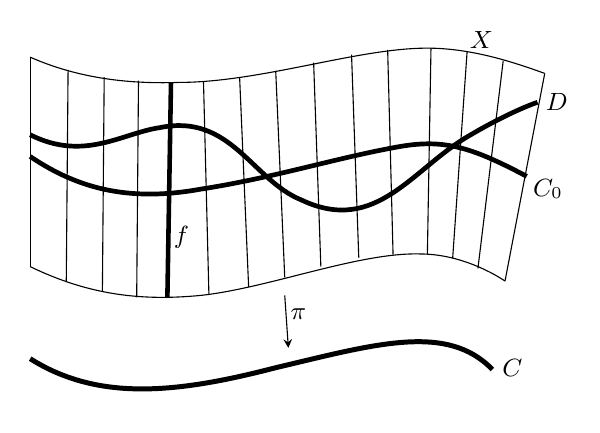
\begin{tikzpicture}[x=.65bp,y=-.65bp,every node/.style={inner sep=1.5pt,font=\small},>=stealth]
\draw[thin] (0,15) .. controls (25,26) and (52,30) .. (82,29)
 .. controls (128,29) and (181,10) .. (220,10)
 .. controls (246,10) and (271,19) .. (285,24);
\draw[thin] (0,131) .. controls (33,147) and (62,150) .. (94,147)
 .. controls (132,143) and (182,123) .. (216,124)
 .. controls (236,124) and (254,133) .. (263,139);
\foreach \xa/\ya/\xb/\yb in {0/15/0/131,21/22/20/139,41/26/40/145,60/28/59/148,96/28.5/99/146.5,116/26/121/142.3,136/22.6/141/137,157/18/161/131,178/13.6/182/126,198/11/201/124.4,222/10/220/124.2,242/12/234/126.4,262/17/248/132,285/24/263/139}
  \draw[thin] (\xa,\ya) -- (\xb,\yb);
\draw[line width=1.65pt] (78,29) -- (76,148);
\draw[line width=1.7pt] (0,58) .. controls (30,73) and (51,57) .. (72,54)
 .. controls (111,46) and (123,83) .. (150,94)
 .. controls (192,114) and (212,76) .. (244,58)
 .. controls (261,48) and (275,42) .. (281,40);
\draw[line width=1.7pt] (0,70) .. controls (28,89) and (57,95) .. (95,88)
 .. controls (134,82) and (169,71) .. (202,65)
 .. controls (228,60) and (243,64) .. (275,81);
\draw[->] (141,147) -- (143,176) node[pos=.35,right] {$\pi$};
\draw[line width=1.8pt] (0,182) .. controls (38,206) and (82,201) .. (136,187)
 .. controls (191,174) and (231,162) .. (256,188);
\node[above] at (250,13) {$X$};
\node[right] at (283,40) {$D$};
\node[right] at (276,88) {$C_0$};
\node[right] at (77,115) {$f$};
\node[right] at (259,187) {$C$};
\end{tikzpicture}\par\nobreak\smallskip
Figure 19.\enspace A ruled surface.\par}

\medskip
\noindent\hypertarget{result-V-2.8.1}{}\textbf{Notation 2.8.1.} For the rest of this section, we fix the following notation (Fig.~\Goto{fig-book-19}{19}). Let $C$ be a curve of genus $g$, and let $\pi\colon X\to C$ be a ruled surface over $C$. We write $X\cong\mathbf P(\mathcal E)$ where $\mathcal E$ satisfies the conditions of \Goto{result-V-2.8}{(2.8)}, in which case we say $\mathcal E$ is \emph{normalized}. This does not necessarily determine $\mathcal E$ uniquely, but it does determine $\deg\mathcal E$. We let $\mathfrak e$ be the divisor on $C$ corresponding to the invertible sheaf $\bigwedge^2\mathcal E$, so that $e=-\deg\mathfrak e$. (This sign is put in for historical reasons.) We fix a section $C_0$ of $X$ with $\mathcal L(C_0)\cong\mathcal O_{\mathbf P(\mathcal E)}(1)$. If $\mathfrak b$ is any divisor on $C$, then we denote the divisor $\pi^*\mathfrak b$ on $X$ by $\mathfrak b f$, by abuse of notation. Thus any element of $\operatorname{Pic}X$ can be written $aC_0+\mathfrak b f$ with $a\in\mathbf Z$ and $\mathfrak b\in\operatorname{Pic}C$. Any element of $\operatorname{Num}X$ can be written $aC_0+bf$ with $a,b\in\mathbf Z$.

\medskip
\noindent\hypertarget{result-V-2.9}{}\textbf{Proposition 2.9.} \emph{If $D$ is any section of $X$, corresponding to a surjection $\mathcal E\to\mathcal L\to0$, and if $\mathcal L=\mathcal L(\mathfrak b)$ for some divisor $\mathfrak b$ on $C$, then $\deg\mathfrak b=C_0\cdot D$, and}
\[
D\sim C_0+(\mathfrak b-\mathfrak e)f.
\]
\emph{In particular, we have $C_0^2=\deg\mathfrak e=-e$.}

\smallskip
\noindent\textsc{Proof.} Since $\mathcal L=\sigma^*(\mathcal L(C_0)\otimes\mathcal O_D)$, we have $\deg\mathcal L=C_0\cdot D$ by \Goto{result-V-1.1}{(1.1)} and \Goto{result-V-1.3}{(1.3)}. Writing
\[
0\to\mathcal N\to\mathcal E\to\mathcal L\to0,
\]
we have $\mathcal L(C_0-D)\cong\pi^*\mathcal N$ by \Goto{result-V-2.6}{(2.6)} and the choice of $C_0$ \Goto{result-V-2.8.1}{(2.8.1)}. But $\mathcal N=\mathcal L(\mathfrak e-\mathfrak b)$, so we have $D\sim C_0+(\mathfrak b-\mathfrak e)f$ in $\operatorname{Pic}X$. Finally, in the case $D=C_0$, $\mathcal N=\mathcal O_C$, so $\mathfrak b=\mathfrak e$ and we have $C_0^2=\deg\mathfrak e=-e$.

\medskip
\noindent\hypertarget{result-V-2.10}{}\textbf{Lemma 2.10.} \emph{The canonical divisor $K$ on $X$ is given by}
\[
K\sim-2C_0+(\mathfrak k+\mathfrak e)f
\]
\emph{where $\mathfrak k$ is the canonical divisor on $C$.}
}
% Contents from body/page-388.tex.
\ChapterSheet{388}{374}{\Goto{p-370}{V\quad Surfaces}}{%
\noindent\textsc{Proof.} Let $K\sim aC_0+\mathfrak b f$. Using the adjunction formula \Goto{result-V-1.5}{(1.5)} for a fibre $f$, we have
\[
-2=f\cdot(f+K)=a.
\]
Now we use the adjunction formula for $C_0$ in its invertible sheaf form (II, \Goto{result-II-8.20}{8.20}), which says that
\[
\omega_{C_0}\cong\omega_X\otimes\mathcal L(C_0)\otimes\mathcal O_{C_0}\cong\mathcal L(-C_0+\mathfrak b f)\otimes\mathcal O_{C_0}.
\]
Identifying $C_0$ with $C$ via $\pi$, the corresponding statement for divisors on $C$ is $\mathfrak k=-\mathfrak e+\mathfrak b$, so $\mathfrak b=\mathfrak e+\mathfrak k$. This result also follows from (III, Ex.~\Goto{ex-III-8.4}{8.4}).

\medskip
\noindent\hypertarget{result-V-2.11}{}\textbf{Corollary 2.11.} \emph{For numerical equivalence, we have}
\[
K\equiv-2C_0+(2g-2-e)f
\]
\emph{and therefore}
\[
K^2=8(1-g).
\]

\smallskip
\noindent\textsc{Proof.} We have $\deg\mathfrak k=2g-2$ (IV, \Goto{result-IV-1.3.3}{1.3.3}) and $\deg\mathfrak e=-e$. Then we compute $K^2$ using \Goto{result-V-2.3}{(2.3)} and \Goto{result-V-2.9}{(2.9)}.

\medskip
\noindent\hypertarget{result-V-2.11.1}{}\textbf{Example 2.11.1.} For any curve $C$, the ruled surface $X=C\times\Proj^1$ corresponds to the (normalized) locally free sheaf $\mathcal E=\mathcal O_C\oplus\mathcal O_C$ on $C$. In this case $e=0$, and $C_0$ is any fibre of the second projection.

\medskip
\noindent\hypertarget{result-V-2.11.2}{}\textbf{Example 2.11.2.} If $C$ is a curve of genus $\geq1$, and $\mathcal E=\mathcal O_C\oplus\mathcal L$ where $\deg\mathcal L=0$ but $\mathcal L\ncong\mathcal O_C$, then there are two choices of normalized $\mathcal E$, namely $\mathcal E$ and $\mathcal E\otimes\mathcal L^{-1}$. We have $e=0$, $\deg\mathfrak e=0$, but $\mathfrak e$ is determined only up to sign. There are exactly two choices of $C_0$, both with $C_0^2=0$.

\medskip
\noindent\hypertarget{result-V-2.11.3}{}\textbf{Example 2.11.3.} On any curve $C$, let $\mathcal E=\mathcal O_C\oplus\mathcal L$ with $\deg\mathcal L<0$. Then the normalized $\mathcal E$ is unique, $\mathcal L=\mathcal L(\mathfrak e)$ and $\mathfrak e$ is unique. The section $C_0$ is unique, with $C_0^2=-e<0$. In this case $e=-\deg\mathcal L>0$.

\medskip
\noindent\hypertarget{result-V-2.11.4}{}\textbf{Example 2.11.4.} Let $C$ be any curve embedded in $\Proj^n$, of degree $d$. Let $X_0$ be the cone over $C$ in $\Proj^{n+1}$, with vertex $P_0$ (I, Ex.~\Goto{ex-I-2.10}{2.10}). If we blow up the point $P_0$, we will show that we obtain a ruled surface $X$ over $C$, of the kind \Goto{result-V-2.11.3}{(2.11.3)} above, with $\mathcal L\cong\mathcal O_C(-1)$. In particular, $e=d$, and the inverse image of $P_0$ in $X$ is the section $C_0$ with $C_0^2=-d$.

First of all, we show that $\Proj^{n+1}$ with one point blown up is isomorphic to $\mathbf P(\mathcal O\oplus\mathcal O(1))$ over $\Proj^n$. Indeed, let $\Proj^{n+1}$ have coordinates $x_0,\ldots,x_{n+1}$. If we blow up the point $P_0=(1,0,\ldots,0)$, then we get the variety $V\subseteq\Proj^n\times\Proj^{n+1}$ defined by the equations $x_i y_j=x_j y_i$ for $i,j=1,2,\ldots,n+1$, where $y_1,\ldots,y_{n+1}$ are the coordinates for $\Proj^n$ (II, \Goto{result-II-7.12.1}{7.12.1}). On the other hand, if $\mathcal E=\mathcal O\oplus\mathcal O(1)$ on $\Proj^n$, then $\mathbf P(\mathcal E)$ is defined as $\operatorname{\mathbf{Proj}}S(\mathcal E)$, where $S(\mathcal E)$ is the symmetric algebra of $\mathcal E$ (II, \Goto{sec-II-7}{\S7}). Now $\mathcal E$ is generated by the global sections $1$ of $\mathcal O$ and $y_1,\ldots,y_{n+1}$ of $\mathcal O(1)$. Therefore $S(\mathcal E)$ is a quotient of the polynomial
}
% Contents from body/page-389.tex.
\ChapterSheet{389}{375}{\Goto{sec-V-2}{2\quad Ruled Surfaces}}{%
algebra $\mathcal O[x_0,\ldots,x_{n+1}]$ by the mapping $x_0\mapsto1$, $x_i\mapsto y_i$ for $i=1,\ldots,n+1$. The kernel of this map is the ideal generated by all $x_i y_j-x_j y_i$, \EditionText{for $i,j=1,\ldots,n+1$}. Therefore $\mathbf P(\mathcal E)$ is isomorphic to the subscheme of $\Proj^n\times\Proj^{n+1}$ defined by these equations, which is the same as the variety $V\subseteq\Proj^n\times\Proj^{n+1}$ defined above. The first projection makes $V$ look like $\mathbf P(\mathcal E)$, the second projection makes $V$ look like blowing up a point.

Now let $Y$ be any subvariety of $\Proj^n$, and $X_0$ its cone in $\Proj^{n+1}$, with vertex $P_0$. If we blow up $P_0$ on $X_0$, we get a variety $X$ which is the strict transform of $X_0$ in $V$ (II, \Goto{result-II-7.15.1}{7.15.1}). On the other hand, this variety $X$ is clearly the inverse image of $Y$ under the projection $\pi\colon V\cong\mathbf P(\mathcal E)\to\Proj^n$. So we see that $X\cong\mathbf P(\mathcal O_Y\oplus\mathcal O_Y(1))$. Twisting by $\mathcal O_Y(-1)$, we still have the same variety, so $X\cong\mathbf P(\mathcal O_Y\oplus\mathcal O_Y(-1))$.

In particular, if $Y$ is a nonsingular curve $C$ of degree $d$ in $\Proj^n$, then $\mathcal L=\mathcal O_C(-1)$ has degree $-d$.

\medskip
\noindent\hypertarget{result-V-2.11.5}{}\textbf{Example 2.11.5.} As a special case of \Goto{result-V-2.11.4}{(2.11.4)}, we see that $\Proj^2$ with one point blown up is isomorphic to the rational ruled surface over $\Proj^1$ defined by $\mathcal E=\mathcal O\oplus\mathcal O(-1)$, having $e=1$.

\medskip
\noindent\hypertarget{result-V-2.11.6}{}\textbf{Example 2.11.6.} For an example of a ruled surface with $e<0$, let $C$ be an elliptic curve, let $P\in C$ be a point, and construct a locally free sheaf $\mathcal E$ of rank $2$ as an extension
\[
0\to\mathcal O\to\mathcal E\to\mathcal L(P)\to0
\]
defined by a nonzero element $\xi\in\operatorname{Ext}^1(\mathcal L(P),\mathcal O)$ (III, Ex.~\Goto{ex-III-6.1}{6.1}). In this case $\operatorname{Ext}^1(\mathcal L(P),\mathcal O)\cong H^1(C,\mathcal L(-P))$ (III, \Goto{result-III-6.3}{6.3}) and (III, \Goto{result-III-6.7}{6.7}). This is dual to $H^0(C,\mathcal L(P))$ which has dimension $1$. Thus $\xi$ is unique up to a scalar multiple, and so $\mathcal E$ is uniquely determined up to isomorphism.

I claim this $\mathcal E$ is normalized. Clearly $H^0(\mathcal E)\ne0$ by construction. If $\mathcal M$ is any invertible sheaf, then we have an exact sequence
\[
0\to\mathcal M\to\mathcal E\otimes\mathcal M\to\mathcal L(P)\otimes\mathcal M\to0.
\]
If $\deg\mathcal M<0$, then we have $H^0(\mathcal M)=0$, and $H^0(\mathcal L(P)\otimes\mathcal M)=0$, and therefore also $H^0(\mathcal E\otimes\mathcal M)=0$, except for the case $\mathcal M=\mathcal L(-P)$. In that case we look at the cohomology sequence
\[
0\to H^0(\mathcal M)\to H^0(\mathcal E\otimes\mathcal M)\to H^0(\mathcal L(P)\otimes\mathcal M)\xrightarrow{\delta}H^1(\mathcal M)\to\cdots\,.
\]
The image of $1\in H^0(\mathcal L(P)\otimes\mathcal M)=H^0(\mathcal O_C)$ by $\delta$ is just the element $\xi$ defining $\mathcal E$ (III, Ex.~\Goto{ex-III-6.1}{6.1}), which is nonzero. Therefore $\delta$ is injective, and again $H^0(\mathcal E\otimes\mathcal M)=0$. Thus $\mathcal E$ is normalized.

Now taking $X=\mathbf P(\mathcal E)$, we have an elliptic ruled surface with $e=-1$.

\medskip
Now that we have established some general properties of ruled surfaces and have given some examples, we can look more closely at some special cases. We begin by discussing the possible values of the invariant $e$.
}
% Contents from body/page-390.tex.
\ChapterSheet{390}{376}{\Goto{p-370}{V\quad Surfaces}}{%
\noindent\hypertarget{result-V-2.12}{}\textbf{Theorem 2.12.} \textit{Let $X$ be a ruled surface over the curve $C$ of genus $g$, determined by a normalized locally free sheaf $\mathcal E$.}

\textit{(a) If $\mathcal E$ is decomposable (i.e., a direct sum of two invertible sheaves) then $\mathcal E\cong\mathcal O_C\oplus\mathcal L$ for some $\mathcal L$ with $\deg\mathcal L\leq0$. Therefore $e\geq0$. All values of $e\geq0$ are possible.}

\textit{(b) If $\mathcal E$ is indecomposable, then $-2g\leq e\leq2g-2$. (In fact, there are even stronger restrictions on $e$ (Ex.~\Goto{ex-V-2.5}{2.5}).)}

\smallskip
\noindent\textsc{Proof.} If $\mathcal E$ is decomposable, then $\mathcal E\cong\mathcal L_1\oplus\mathcal L_2$ for two invertible sheaves $\mathcal L_1$ and $\mathcal L_2$ on $C$. We must have $\deg\mathcal L_i\leq0$ because of the normalization \Goto{result-V-2.8}{(2.8)} and furthermore $H^0(\mathcal L_i)\ne0$ for at least one of them. Thus one of them is $\mathcal O_C$, so we have $\mathcal E\cong\mathcal O_C\oplus\mathcal L$ with $\deg\mathcal L\leq0$. From \Goto{result-V-2.11.1}{(2.11.1)}, \Goto{result-V-2.11.2}{(2.11.2)}, and \Goto{result-V-2.11.3}{(2.11.3)}, we see that all values of $e\geq0$ are possible.

Now suppose $\mathcal E$ is indecomposable. Then, corresponding to the section $C_0$, we have an exact sequence
\[
0\to\mathcal O_C\to\mathcal E\to\mathcal L\to0
\]
for some $\mathcal L$ \Goto{result-V-2.8}{(2.8)}. This must be a nontrivial extension, so it corresponds to a nonzero element $\xi\in\operatorname{Ext}^1(\mathcal L,\mathcal O_C)\cong H^1(C,\mathcal L^\vee)$ (III, Ex.~\Goto{ex-III-6.1}{6.1}). In particular, $H^1(\mathcal L^\vee)\ne0$, so we must have $\deg\mathcal L^\vee\leq2g-2$ (IV, \Goto{result-IV-1.3.4}{1.3.4}). Since $e=-\deg\mathcal L$, we have $e\leq2g-2$.

On the other hand, we have $H^0(\mathcal E\otimes\mathcal M)=0$ for all $\deg\mathcal M<0$ by the normalization. In particular, taking $\deg\mathcal M=-1$, we have
\[
0=H^0(\mathcal E\otimes\mathcal M)\to H^0(\mathcal L\otimes\mathcal M)\to H^1(\mathcal M)\to\cdots\,,
\]
so we must have
\[
\dim H^0(\mathcal L\otimes\mathcal M)\leq\dim H^1(\mathcal M).
\]
Since $\deg\mathcal M<0$, $H^0(\mathcal M)=0$, so by Riemann--Roch, we have $\dim H^1(\mathcal M)=g$. On the other hand, also by Riemann--Roch, we have
\[
\dim H^0(\mathcal L\otimes\mathcal M)\geq\deg\mathcal L-1+1-g.
\]
Combining, we get $\deg\mathcal L\leq2g$, hence $e\geq-2g$.

\medskip
\noindent\hypertarget{result-V-2.13}{}\textbf{Corollary 2.13.} \textit{If $g=0$, then $e\geq0$, and for each $e\geq0$ there is exactly one rational ruled surface with invariant $e$, given by $\mathcal E=\mathcal O\oplus\mathcal O(-e)$ over $C=\Proj^1$.}

\smallskip
\noindent\textsc{Proof.} If $g=0$, case (b) of \Goto{result-V-2.12}{(2.12)} cannot occur. Hence $\mathcal E\cong\mathcal O_C\oplus\mathcal L$. But the only invertible sheaves on $\Proj^1$ are $\mathcal O(n)$ for $n\in\mathbb Z$ (II, \Goto{result-II-6.4}{6.4}). So for each $e\geq0$ there is just one possibility.

\medskip
\noindent\hypertarget{result-V-2.14}{}\textbf{Corollary 2.14.} \textit{Every locally free sheaf $\mathcal E$ of rank $2$ on $\Proj^1$ is decomposable.}

\smallskip
\noindent\textsc{Proof.} After tensoring with a suitable invertible sheaf, it becomes normalized, in which case it is isomorphic to $\mathcal O\oplus\mathcal O(-e)$ by \Goto{result-V-2.13}{(2.13)}. See (Ex.~\Goto{ex-V-2.6}{2.6}) for a generalization.
}
% Contents from body/page-391.tex.
\ChapterSheet{391}{377}{\Goto{sec-V-2}{2\quad Ruled Surfaces}}{%
\noindent\hypertarget{result-V-2.15}{}\textbf{Theorem 2.15.} \textit{If $X$ is a ruled surface over an elliptic curve $C$, corresponding to an indecomposable $\mathcal E$, then $e=0$ or $-1$, and there is exactly one such ruled surface over $C$ for each of these two values of $e$.}

\smallskip
\noindent\textsc{Proof.} According to \Goto{result-V-2.12}{(2.12)} we must have $e=0,-1,-2$. If $e=0$, then we have an exact sequence
\[
0\to\mathcal O_C\to\mathcal E\to\mathcal L\to0
\]
with $\deg\mathcal L=0$. This extension corresponds to a nonzero element $\xi\in H^1(\mathcal L^\vee)$. In particular, $H^1(\mathcal L^\vee)\ne0$. It is dual to $H^0(\mathcal L)$, so we must have $\mathcal L\cong\mathcal O_C$. Conversely, taking $\mathcal L=\mathcal O_C$, we have $\dim H^1(\mathcal O_C)=1$, so there is just one choice of nonzero $\xi\in H^1(\mathcal O_C)$, up to isomorphism, which is a nontrivial extension
\[
0\to\mathcal O_C\to\mathcal E\to\mathcal O_C\to0.
\]
Clearly this $\mathcal E$ is normalized. Furthermore, this $\mathcal E$ is indecomposable, because if $\mathcal E$ were decomposable, being normalized, it would be isomorphic to $\mathcal O_C\oplus\mathcal L$ for some $\mathcal L$, by \Goto{result-V-2.12}{(2.12)}. But $\bigwedge^2\mathcal E\cong\mathcal O_C$, so $\mathcal L\cong\mathcal O_C$, so in fact this extension would have to split, which it doesn't. Thus we get exactly one elliptic ruled surface $X$ with $e=0$ and $\mathcal E$ indecomposable.

If $e=-1$, then we have an exact sequence
\[
0\to\mathcal O_C\to\mathcal E\to\mathcal L(P)\to0
\]
for some point $P\in C$, because every invertible sheaf of degree $1$ on $C$ is of the form $\mathcal L(P)$ (IV, \Goto{result-IV-1.3.7}{1.3.7}). Furthermore, for each $P$ there exists such a normalized bundle, unique up to isomorphism, by \Goto{result-V-2.11.6}{(2.11.6)}. To show that there is just one elliptic ruled surface with $e=-1$, it will be sufficient to show that if $\mathcal E$ is defined by $P$ as above, and $\mathcal E'$ is similarly defined by $Q\ne P$, then there exists an invertible sheaf $\mathcal M$ on $C$ such that $\mathcal E'\cong\mathcal E\otimes\mathcal M$.

\EditionText{The map defined by $|P+Q|$ has degree two and is separable in every characteristic. Indeed, a purely inseparable map would preserve the genus (IV, \Goto{result-IV-2.5}{2.5}). Hurwitz's theorem (IV, \Goto{result-IV-2.4}{2.4}) gives a ramification divisor of degree four, so there is a ramified point $R$ with fibre divisor $2R\sim P+Q$. As $P\ne Q$, the fibre containing $P$ is the reduced divisor $P+Q$, so $R\ne P$.}
We will show that $\mathcal E'\cong\mathcal E\otimes\mathcal L(R-P)$. In any case, we have an exact sequence
\[
0\to\mathcal L(R-P)\to\mathcal E\otimes\mathcal L(R-P)\to\mathcal L(R)\to0.
\]
Since $H^0(\mathcal L(R))\ne0$ and $H^1(\mathcal L(R-P))=0$, we see that $H^0(\mathcal E\otimes\mathcal L(R-P))\ne0$. So we get an exact sequence
\[
0\to\mathcal O_C\to\mathcal E\otimes\mathcal L(R-P)\to\mathcal N\to0,
\]
and the quotient $\mathcal N$ must be invertible, as in the proof of \Goto{result-V-2.8}{(2.8)}. So we have
\[
\mathcal N\cong\bigwedge^2(\mathcal E\otimes\mathcal L(R-P))\cong
(\bigwedge^2\mathcal E)\otimes\mathcal L(2R-2P).
\]
Since $\bigwedge^2\mathcal E\cong\mathcal L(P)$, we have $\mathcal N\cong\mathcal L(2R-P)\cong\mathcal L(Q)$. Therefore $\mathcal E\otimes\mathcal L(R-P)\cong\mathcal E'$ as required. This proves the uniqueness of the elliptic ruled surface with $e=-1$.
}
% Contents from body/page-392.tex.
\ChapterSheet{392}{378}{\Goto{p-370}{V\quad Surfaces}}{%
Finally, we will show that the case $e=-2$ does not occur. If it did, we would have a normalized bundle $\mathcal E$ with an exact sequence
\[
0\longrightarrow\mathcal O_C\longrightarrow\mathcal E\longrightarrow\mathcal L(P+Q)\longrightarrow0
\]
\noindent for some $P,Q\in C$, since every invertible sheaf of degree $2$ is of the form $\mathcal L(P+Q)$. Now take any pair of points $R,S\in C$ with $R+S\sim P+Q$, and let $\mathcal M=\mathcal L(-R)$. Then, since $\mathcal E$ is normalized, $H^0(\mathcal E\otimes\mathcal M)=0$, so the map $\gamma\colon H^0(\mathcal L(P+Q-R))\to H^1(\mathcal L(-R))$ must be injective. On the other hand, let $\xi\in H^1(\mathcal L(-P-Q))$ be the element defining the extension $\mathcal E$. Then we have a commutative diagram, writing $\mathcal L(P+Q-R)$ as $\mathcal L(S)$,
\begin{center}
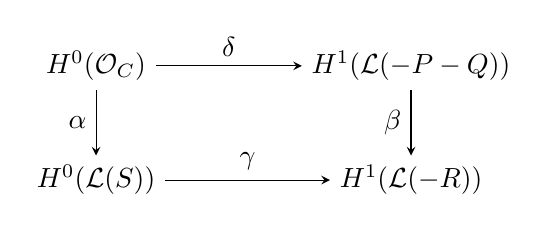
\begin{tikzpicture}[>=stealth,x=1cm,y=1cm]
\node (a) at (0,0) {$H^0(\mathcal O_C)$};
\node (b) at (4,0) {$H^1(\mathcal L(-P-Q))$};
\node (c) at (0,-1.45) {$H^0(\mathcal L(S))$};
\node (d) at (4,-1.45) {$H^1(\mathcal L(-R))$};
\draw[->] (a)--node[above]{$\delta$}(b);
\draw[->] (a)--node[left]{$\alpha$}(c);
\draw[->] (b)--node[left]{$\beta$}(d);
\draw[->] (c)--node[above]{$\gamma$}(d);
\end{tikzpicture}
\end{center}
\noindent where $\delta(1)=\xi$, $\alpha(1)=t$, a nonzero section defining the divisor $S$, and $\beta$ is induced from the map $\mathcal O_C\to\mathcal L(S)$ corresponding to $t$. Now $\beta$ is dual to the map
\[
\beta'\colon H^0(\mathcal L(R))\longrightarrow H^0(\mathcal L(P+Q))
\]
\noindent also induced by $t$. The image of any nonzero element of $H^0(\mathcal L(R))$ by $\beta'$ is a section of $H^0(\mathcal L(P+Q))$ corresponding to the effective divisor $R+S\in|P+Q|$.

By varying $R$ and $S$, we get every divisor in the linear system $|P+Q|$. Therefore the image of $\beta'$ as $R$ varies fills up the whole $2$-dimensional vector space $H^0(\mathcal L(P+Q))$. In particular, we can choose $R$ so that the image of $\beta'$ lands in the kernel of $\xi$, considered as a linear functional on $H^0(\mathcal L(P+Q))$. In that case, $\beta(\xi)=0$, which contradicts the injectivity of $\gamma$. Thus the case $e=-2$ is impossible.

\medskip
\noindent\hypertarget{result-V-2.15.1}{}\textbf{Caution 2.15.1.} One point which came up in the first part of this proof should be noted. It is possible for a locally free sheaf of rank $2$ to be a nontrivial extension of two invertible sheaves, and yet be decomposable. For example, the sheaf of differentials on $\Proj^1$ is isomorphic to $\mathcal O(-2)$, so we have an exact sequence (II, \Goto{result-II-8.13}{8.13})
\[
0\longrightarrow\mathcal O(-2)\longrightarrow\mathcal O(-1)\oplus\mathcal O(-1)
 \longrightarrow\mathcal O\longrightarrow0.
\]
\noindent The sequence cannot be split (because for example $H^0(\mathcal O(-1)\oplus\mathcal O(-1))=0$), but the sheaf in the middle is decomposable.

\medskip
\noindent\hypertarget{result-V-2.16}{}\textbf{Corollary 2.16} (Atiyah). \emph{For each integer $n$, there is a natural one-to-one correspondence (described explicitly in the proof below) between the set of isomorphism classes of indecomposable locally free sheaves of rank $2$ and degree $n$ on the elliptic curve $C$, and the set of points of $C$.}
}
% Contents from body/page-393.tex.
\ChapterSheet{393}{379}{\Goto{sec-V-2}{2\quad Ruled Surfaces}}{%
\Proof Fix a point $P_0\in C$. Let $\mathcal E'$ be an indecomposable locally free sheaf of rank $2$ and degree $n$ on $C$. Tensoring with $\mathcal L(mP_0)$ for some $m$, we may assume $n=0$ or $1$. If $n=0$, then by (\Goto{result-V-2.2}{2.2}), (\Goto{result-V-2.8}{2.8}), and (\Goto{result-V-2.15}{2.15}) there is a (unique) invertible sheaf $\mathcal L$ of degree $0$ on $C$ such that $\mathcal E'\otimes\mathcal L$ is isomorphic to the unique nontrivial extension of $\mathcal O_C$ by $\mathcal O_C$. Since the invertible sheaves of degree $0$ are in one-to-one correspondence with the closed points of $C$ (IV, \S\Goto{sec-IV-4}{4}), we have the result. If $n=1$, then as in the proof of (\Goto{result-V-2.15}{2.15}) we find that $\mathcal E'$ is an extension of $\mathcal L(P)$ by $\mathcal O_C$ for some uniquely determined point $P\in C$, whence the result.

\medskip
\noindent\hypertarget{result-V-2.16.1}{}\textbf{Remark 2.16.1.} More generally, for any curve $C$, of genus $g$, one can consider the problem of classifying all locally free sheaves $\mathcal E$ on $C$ up to isomorphism. The rank $r$ and the degree $d$ (which is $\deg\bigwedge^r\mathcal E$) are numerical invariants. For fixed $r$ and $d$, one expects some kind of continuous family. For $g=0$, all locally free sheaves are direct sums of invertible sheaves (Ex.~\Goto{ex-V-2.6}{2.6}). For $g=1$ the general classification, which is similar to the rank $2$ case we have just done, has been accomplished by Atiyah \Goto{bib-atiyah-1}{[1]}. For $g\ge2$, the situation becomes more complicated. Among the indecomposable locally free sheaves, one has to distinguish between the \emph{stable} ones (Ex.~\Goto{ex-V-2.8}{2.8}) in the sense of Mumford \Goto{bib-480-3}{[1]}, and the rest. The stable ones form nice algebraic families, whereas the others do not. See for example, Narasimhan and Seshadri \Goto{bib-narasimhan-seshadri-1}{[1]}. Similarly, for the ruled surfaces themselves, the ones with $e<0$ are \emph{stable}, and form nice algebraic families, but the others do not.

\smallskip
Next we will study the rational ruled surfaces, which were classified in (\Goto{result-V-2.13}{2.13}).

\medskip
\noindent\hypertarget{result-V-2.17}{}\textbf{Theorem 2.17.} \emph{Let $X_e$, for any $e\ge0$, be the rational ruled surface defined by $\mathcal E=\mathcal O\oplus\mathcal O(-e)$ on $C=\Proj^1$ \textup{(\Goto{result-V-2.13}{2.13})}. Then:}
\begin{parts}
\item\hypertarget{result-V-2.17a}{} \emph{there is a section $D\sim C_0+nf$ if and only if $n=0$ or $n\ge e$. In particular, there is a section $C_1\sim C_0+ef$ with $C_0\cap C_1=\varnothing$ and $C_1^2=e$;}
\item\hypertarget{result-V-2.17b}{} \emph{the linear system $|C_0+nf|$ is base-point-free if and only if $n\ge e$;}
\item\hypertarget{result-V-2.17c}{} \emph{the linear system $|C_0+nf|$ is very ample if and only if $n>e$.}
\end{parts}

\Proof\par
(\Goto{result-V-2.17a}{a}) According to (\Goto{result-V-2.6}{2.6}) and (\Goto{result-V-2.9}{2.9}), giving a section $D\sim C_0+nf$ is equivalent to giving a surjective map $\mathcal E\to\mathcal L\to0$ with $\deg\mathcal L=C_0.D=n-e$. Since we are on $\Proj^1$, this means a surjective map
\[
\mathcal O\oplus\mathcal O(-e)\longrightarrow\mathcal O(n-e)\longrightarrow0.
\]
\noindent If $n<e$, there are no nonzero maps of $\mathcal O$ to $\mathcal O(n-e)$, so the map $\mathcal O(-e)\to\mathcal O(n-e)$ must be an isomorphism, and therefore $n=0$. This corresponds to the section $C_0$, which is unique if $e>0$. Otherwise we have $n\ge e$, and any such $n$ is possible. We have only to take maps $\mathcal O\to\mathcal O(n-e)$ and $\mathcal O(-e)\to\mathcal O(n-e)$ corresponding to effective divisors of degrees $n-e$ and $n$ on $C$ which do not meet. Then the corresponding map $\mathcal O\oplus\mathcal O(-e)\to\mathcal O(n-e)$ will be surjective.
}
% Contents from body/page-394.tex.
\ChapterSheet{394}{380}{\Goto{p-370}{V\quad Surfaces}}{%
In particular, if we take $n=e$, there is a section $C_1\sim C_0+ef$. Then $C_1^2=e$, and $C_0.C_1=0$, so $C_0\cap C_1=\varnothing$.

(\Goto{result-V-2.17b}{b}) If $|C_0+nf|$ is base-point-free, then $C_0.(C_0+nf)\ge0$ so $n\ge e$. Conversely, if $n\ge e$, then $C_0+nf\sim C_1+(n-e)f$, and since $C_0\cap C_1=\varnothing$, and any $f$ is linearly equivalent to any other, we can find a divisor of the form $C_0+nf$ or $C_1+(n-e)f$ which misses any given point.

(\Goto{result-V-2.17c}{c}) If $D=C_0+nf$ is very ample, then we must have $D.C_0>0$, so $n>e$. Conversely, suppose $n>e$. Then we will show that $D$ is very ample by showing that the linear system $|D|$ separates points and tangent vectors (II, \Goto{result-II-7.8.2}{7.8.2}).

\emph{Case 1.} Let $P\ne Q$ be two points not both in $C_0$, and not both in any fibre. Then a divisor of the form $C_0+nf$ for suitable $f$ will separate them.

\emph{Case 2.} Let $P$ be a point and $t$ a tangent vector at $P$, such that $P,t$ are not both in $C_0$ and not both in any fibre. Then a divisor of the form $C_0+\sum_{i=1}^n f_i$, for suitable fibres $f_i$, will contain $P$ but not $t$.

\emph{Case 3.} Suppose $P,Q$ or $P,t$ are both in $C_0$. Then a divisor of the form $C_1+\sum_{i=1}^{n-e}f_i$ will separate them.

\emph{Case 4.} Suppose $P,Q$, or $P,t$ are both in the same fibre $f$. Since $D.f=1$, the invertible sheaf $\mathcal L(D)\otimes\mathcal O_f$ is very ample on $f\cong\Proj^1$. Thus to separate $P,Q$ or $P,t$, it will be sufficient to show that the natural map $H^0(X,\mathcal L(D))\to H^0(f,\mathcal L(D)\otimes\mathcal O_f)$ is surjective. The cokernel of this map lands in $H^1(X,\mathcal L(D-f))$, which by (\Goto{result-V-2.4}{2.4}) is isomorphic to $H^1(C,\pi_*\mathcal L(D-f))$. On the other hand, $D-f\sim C_0+(n-1)f$, so
\[
\pi_*(\mathcal L(D-f))\cong\pi_*(\mathcal L(C_0))\otimes\mathcal O_C(n-1)
\]
\noindent by the projection formula (II, Ex.~\Goto{ex-II-5.1}{5.1}). Now $\pi_*(\mathcal L(C_0))\cong\mathcal E$ by (\Goto{result-V-2.8}{2.8}) and (II, \Goto{result-II-7.11}{7.11}), so we have
\[
\pi_*(\mathcal L(D-f))\cong\mathcal O(n-1)\oplus\mathcal O(n-e-1).
\]
\noindent Since $n>e\ge0$, both $n-1\ge0$ and $n-e-1\ge0$, so $H^1=0$ and the above map is surjective.\hfill q.e.d.

\medskip
\noindent\hypertarget{result-V-2.18}{}\textbf{Corollary 2.18.} \emph{Let $D$ be the divisor $aC_0+bf$ on the rational ruled surface $X_e$, $e\ge0$. Then:}
\begin{parts}
\item\hypertarget{result-V-2.18a}{} \emph{$D$ is very ample $\Leftrightarrow D$ is ample $\Leftrightarrow a>0$ and $b>ae$;}
\item\hypertarget{result-V-2.18b}{} \emph{the linear system $|D|$ contains an irreducible nonsingular curve $\Leftrightarrow$ it contains an irreducible curve $\Leftrightarrow$ $a=0$, $b=1$ (namely $f$); or $a=1$, $b=0$ (namely $C_0$); or $a>0$, $b>ae$; or $e>0$, $a>0$, $b=ae$.}
\end{parts}

\Proof\par
(\Goto{result-V-2.18a}{a}) If $D$ is very ample, it is certainly ample (II, \Goto{result-II-7.4.3}{7.4.3}). If $D$ is ample, then $D.f>0$, so $a>0$, and $D.C_0>0$, so $b>ae$ (\Goto{result-V-1.6.2}{1.6.2}). Now suppose that $a>0$ and $b>ae$. Then we can write $D=(a-1)(C_0+ef)+(C_0+(b-ae+e)f)$. Since $|C_0+ef|$ has no base points, and $C_0+(b-ae+e)f$ is very ample (\Goto{result-V-2.17}{2.17}), we conclude that $D$ is also very ample (II, Ex.~\Goto{ex-II-7.5}{7.5}).
}
% Contents from body/page-395.tex.
\ChapterSheet{395}{381}{\Goto{sec-V-2}{2\quad Ruled Surfaces}}{%
(\Goto{result-V-2.18b}{b}) If $|D|$ contains an irreducible nonsingular curve, then in particular it contains an irreducible curve. If $D$ is an irreducible curve, then $D$ could be $f$ (in which case $a=0$, $b=1$) or $C_0$ (in which case $a=1$, $b=0$). Otherwise, $\pi$ maps $D$ surjectively to $C$, so $D.f=a>0$, and $D.C_0\ge0$, so $b\ge ae$. If $e=0$ and $b=ae$, then $b=0$ so $D=aC_0$. But in this case $X_0$ is $\Proj^1\times\Proj^1$, and $C_0$ is one of the rulings, so for $D$ to be irreducible, we must have $a=1$. Thus the restrictions on $a,b$ are necessary. To complete the proof, we must show that if $a>0$, $b>ae$, or $e>0$, $a>0$, $b=ae$, then $|D|$ contains an irreducible nonsingular curve. In the first case, $D$ is very ample by (\Goto{result-V-2.18a}{a}), so the result follows from Bertini's theorem (II, \Goto{result-II-8.18}{8.18}) applied to $X$. In the second case, we use the fact (\Goto{result-V-2.11.4}{2.11.4}) that $X_e$ can be obtained from the cone $Y$ over a nonsingular rational curve $C$ of degree $e>0$ in some $\Proj^n$, by blowing up the vertex. In this case, the curve $C_1$ on $X_e$ is the strict transform of the hyperplane section $H$ of $Y$. By Bertini's theorem applied to the very ample divisor $aH$ on $Y$ (II, \Goto{result-II-8.18.1}{8.18.1}), we can find an irreducible nonsingular curve in the linear system $|aH|$, not containing the vertex of $Y$. Its strict transform on $X_e$ is then an irreducible nonsingular curve in the linear system $|aC_1|=|D|$.

\medskip
\noindent\hypertarget{result-V-2.18.1}{}\textbf{Remark 2.18.1.} In case $e=0$, we get some new proofs of earlier results about curves on the nonsingular quadric surface, which is isomorphic to $X_0$ (II, \Goto{result-II-7.6.2}{7.6.2}), (III, Ex.~\Goto{ex-III-5.6}{5.6}), (\Goto{result-V-1.10.1}{1.10.1}).

\medskip
\noindent\hypertarget{result-V-2.19}{}\textbf{Corollary 2.19.} \emph{For every $n>e\ge0$, there is an embedding of the rational ruled surface $X_e$ as a rational scroll of degree $d=2n-e$ in $\Proj^{d+1}$.} (A \emph{scroll} is a ruled surface embedded in $\Proj^N$ in such a way that all the fibres $f$ have degree $1$.)

\Proof Use the very ample divisor $D=C_0+nf$. Then $D.f=1$, so the image of $X_e$ in $\Proj^N$ is a scroll, and $D^2=2n-e$, so the image has degree $d=2n-e$. To find $N$, we compute $H^0(X,\mathcal L(D))$. As in the proof of (\Goto{result-V-2.17}{2.17}), we find that
\[
\begin{aligned}
H^0(X,\mathcal L(D))&=H^0(C,\pi_*\mathcal L(D))\\
  &=H^0(C,\mathcal E\otimes\mathcal O(n))=H^0(\mathcal O(n)\oplus\mathcal O(n-e)).
\end{aligned}
\]
\noindent This has dimension $2n+2-e$, so $N=2n+1-e=d+1$.

\medskip
\noindent\hypertarget{result-V-2.19.1}{}\textbf{Example 2.19.1.} For $e=0$, $n=1$, we recover the nonsingular quadric surface in $\Proj^3$.

For $e=1$, $n=2$, we get a rational scroll of degree $3$ in $\Proj^4$, which is isomorphic to $\Proj^2$ with one point blown up (II, Ex.~\Goto{ex-II-7.7}{7.7}).

In $\Proj^5$, there are two different kinds of rational scrolls of degree $4$, corresponding to $e=0$, $n=2$, and $e=2$, $n=3$.

\medskip
\noindent\hypertarget{result-V-2.19.2}{}\textbf{Remark 2.19.2.} In fact, it is known that every nonsingular surface of degree $d$ in $\Proj^{d+1}$, not contained in any hyperplane, is either one of these rational scrolls (\Goto{result-V-2.19}{2.19}), or $\Proj^2\subseteq\Proj^2$ (if $d=1$), or the Veronese surface in $\Proj^5$ (I, Ex.~\Goto{ex-I-2.13}{2.13}). See, for example, Nagata [\Goto{bib-nagata-5}{5}, I, Theorem 7, p.~365].
}
% Contents from body/page-396.tex.
\ChapterSheet{396}{382}{\Goto{p-370}{V\quad Surfaces}}{%
Now we will try to determine the ample divisors on a ruled surface over a curve of any genus, as an application of Nakai's criterion (\Goto{result-V-1.10}{1.10}). In order to apply Nakai's criterion, we need to know which numerical equivalence classes of divisors on the surface contain an irreducible curve. On a general ruled surface, we cannot expect to get nearly as precise an answer to this question as in the case of the rational ruled surfaces (\Goto{result-V-2.18}{2.18}), but at least we can get some estimates which allow us to apply Nakai's criterion successfully.

\medskip
\noindent\hypertarget{result-V-2.20}{}\textbf{Proposition 2.20.} \emph{Let $X$ be a ruled surface over a curve $C$, with invariant $e\ge0$.}
\begin{parts}
\item\hypertarget{result-V-2.20a}{} \emph{If $Y\equiv aC_0+bf$ is an irreducible curve $\ne C_0,f$, then $a>0$, $b\ge ae$.}
\item\hypertarget{result-V-2.20b}{} \emph{A divisor $D\equiv aC_0+bf$ is ample if and only if $a>0$, $b>ae$.}
\end{parts}
\Proof\par
(\Goto{result-V-2.20a}{a}) Since $Y\ne f$, $\pi\colon Y\to C$ is surjective, so $Y.f=a>0$. Also since $Y\ne C_0$, $Y.C_0=b-ae\ge0$.

(\Goto{result-V-2.20b}{b}) If $D$ is ample, then $D.f=a>0$, and $D.C_0=b-ae>0$. Conversely, if $a>0$, $b-ae>0$, then $D.f>0$, $D.C_0>0$, $D^2=2ab-a^2e>0$ and if $Y=a'C_0+b'f$ is any irreducible curve $\ne C_0,f$, then
\[
D.Y=ab'+a'b-aa'e>aa'e+aa'e-aa'e=aa'e\ge0.
\]
\noindent Therefore by (\Goto{result-V-1.10}{1.10}) $D$ is ample.

\medskip
\noindent\hypertarget{result-V-2.21}{}\textbf{Proposition 2.21.} \emph{Let $X$ be a ruled surface over a curve $C$ of genus $g$, with invariant $e<0$, and assume furthermore either $\operatorname{char}k=0$ or $g\le1$.}
\begin{parts}
\item\hypertarget{result-V-2.21a}{} \emph{If $Y\equiv aC_0+bf$ is an irreducible curve $\ne C_0,f$, then either $a=1$, $b\ge0$ or $a\ge2$, $b\ge\frac12ae$.}
\item\hypertarget{result-V-2.21b}{} \emph{A divisor $D\equiv aC_0+bf$ is ample if and only if $a>0$, $b>\frac12ae$.}
\end{parts}
\Proof\par
(\Goto{result-V-2.21a}{a}) We will use Hurwitz's theorem (IV, \Goto{result-IV-2.4}{2.4}) to get some information about $Y$. Let $\widetilde Y$ be the normalization of $Y$, and consider the composition of the natural map $\widetilde Y\to Y$ with the projection $\pi\colon Y\to C$. If $\operatorname{char}k=0$, this map is a finite, separable map of degree $a$, so by (IV, \Goto{result-IV-2.4}{2.4}) we have
\[
2g(\widetilde Y)-2=a(2g-2)+\deg R,
\]
\noindent where $R$ is the (effective) ramification divisor. On the other hand, $p_a(Y)\ge g(\widetilde Y)$ by (IV, Ex.~\Goto{ex-IV-1.8}{1.8}), so we find that
\[
2p_a(Y)-2\ge a(2g-2).
\]
\noindent Furthermore, this last inequality is true in any characteristic if $g=0,1$, since in any case $p_a(Y)\ge g$ (IV, \Goto{result-IV-2.5.4}{2.5.4}).

By the adjunction formula (\Goto{result-V-1.5}{1.5}), we have
\[
2p_a(Y)-2=Y.(Y+K).
\]
}
% Contents from body/page-397.tex.
\ChapterSheet{397}{383}{\Goto{sec-V-2}{2\quad Ruled Surfaces}}{%
\noindent Substituting $Y\equiv aC_0+bf$ and $K\equiv-2C_0+(2g-2-e)f$ from (\Goto{result-V-2.11}{2.11}), and combining with the inequality above, we find that
\[
b(a-1)\ge\tfrac12ae(a-1).
\]
\noindent Therefore if $a\ge2$, we have $b\ge\frac12ae$ as required. Now $Y.f=a>0$ in any case, so it remains to show that if $a=1$, then $b\ge0$. In the case $a=1$, $Y$ is a section, corresponding to a surjective map $\mathcal E\to\mathcal L\to0$. Because of the normalization of $\mathcal E$, we must have $\deg\mathcal L\ge\deg\mathcal E$. But $\deg\mathcal L=C_0.Y$ (\Goto{result-V-2.9}{2.9}), so we have $b-e\ge-e$, hence $b\ge0$.

(\Goto{result-V-2.21b}{b}) If $D$ is ample, then $D.f=a>0$, and $D^2=2ab-a^2e>0$, so $b>\frac12ae$. Conversely, if $a>0$, $b>\frac12ae$, then $D.f>0$, $D^2>0$, $D.C_0=b-ae>-\frac12ae>0$, and if $Y\equiv a'C_0+b'f$ is any irreducible curve $\ne C_0,f$, then
\[
D.Y=ab'+a'b-aa'e.
\]
\noindent Now if $a'=1$, then $b'\ge0$, so $D.Y>\frac12ae-ae=-\frac12ae>0$. If $a'\ge2$, then $b'\ge\frac12a'e$, so $D.Y>\frac12aa'e+\frac12aa'e-aa'e=0$. Therefore by (\Goto{result-V-1.10}{1.10}), $D$ is ample.

\medskip
\noindent\hypertarget{result-V-2.21.1}{}\textbf{Remark 2.21.1.} In the remaining case $e<0$, $\operatorname{char}k=p>0$, $g\ge2$, we cannot get necessary and sufficient conditions for $D$ to be ample, but it is possible to get some partial results (Ex.~\Goto{ex-V-2.14}{2.14}) and (Ex.~\Goto{ex-V-2.15}{2.15}).

\medskip
\noindent\hypertarget{result-V-2.22.2}{}\hypertarget{result-V-2.21.2}{}\textbf{Remark \EditionText{2.21.2}.} The determination of the very ample divisors on a ruled surface with $g\ge1$ is more subtle than in the rational case (\Goto{result-V-2.18}{2.18}), because it does not depend only on the numerical equivalence class of the divisor (Ex.~\Goto{ex-V-2.11}{2.11}) and (Ex.~\Goto{ex-V-2.12}{2.12}).

\smallskip
\emph{References for \S\Goto{sec-V-2}{2}.} Since the theory of ruled surfaces is very old, I cannot trace the origins of the results given here. Instead, let me simply list a few recent references: Atiyah \Goto{bib-atiyah-1}{[1]}, Hartshorne \Goto{bib-477-5}{[4]}, Maruyama \Goto{bib-479-15-item-1}{[1]}, Nagata \Goto{bib-nagata-5}{[5]}, Shafarevich [\Goto{bib-482-6}{1}, Ch.~IV, V], Tjurin \Goto{bib-tjurin-1}{[1]}, \Goto{bib-482-18}{[2]}.

\Exercises
{\fontsize{9}{10.6}\selectfont\setlength{\parskip}{0pt}
\begin{description}[style=multiline,labelwidth=1.8em,leftmargin=2.15em,itemsep=3pt,topsep=0pt,parsep=0pt]
\item[\hypertarget{ex-V-2.1}{}2.1.] If $X$ is a birationally ruled surface, show that the curve $C$, such that $X$ is birationally equivalent to $C\times\Proj^1$, is unique (up to isomorphism).
\item[\hypertarget{ex-V-2.2}{}2.2.] Let $X$ be the ruled surface $\Proj(\mathcal E)$ over a curve $C$. Show that $\mathcal E$ is decomposable if and only if there exist two sections $C',C''$ of $X$ such that $C'\cap C''=\varnothing$.
\item[\hypertarget{ex-V-2.3}{}2.3.]
\begin{parts}
\item If $\mathcal E$ is a locally free sheaf of rank $r$ on a (nonsingular) curve $C$, then there is a sequence
\[
0=\mathcal E_0\subseteq\mathcal E_1\subseteq\cdots\subseteq\mathcal E_r=\mathcal E
\]
of subsheaves such that $\mathcal E_i/\mathcal E_{i-1}$ is an invertible sheaf for each $i=1,\ldots,r$. We say that $\mathcal E$ is a \emph{successive extension} of invertible sheaves. [\emph{Hint:} Use (II, Ex.~\Goto{ex-II-8.2}{8.2}).]
\end{parts}
\end{description}
}
}
% Contents from body/page-398.tex.
\ChapterSheet{398}{384}{\Goto{p-370}{V\quad Surfaces}}{%
{\fontsize{9}{10.35}\selectfont\setlength{\parskip}{0pt}
\begin{description}[style=multiline,labelwidth=1.8em,leftmargin=2.15em,itemsep=3pt,topsep=0pt,parsep=0pt]
\item[]
\begin{parts}
\item[(b)] Show that this is false for varieties of dimension $\ge2$. In particular, the sheaf of differentials $\Omega$ on $\Proj^2$ is not an extension of invertible sheaves.
\end{parts}
\item[\hypertarget{ex-V-2.4}{}2.4.] Let $C$ be a curve of genus $g$, and let $X$ be the ruled surface $C\times\Proj^1$. We consider the question, for what integers $s\in\mathbf Z$ does there exist a section $D$ of $X$ with $D^2=s$? First show that $s$ is always an even integer, say $s=2r$.
\begin{parts}
\item Show that $r=0$ and any $r\ge g+1$ are always possible. Cf. (IV, Ex.~\Goto{ex-IV-6.8}{6.8}).
\item If $g=3$, show that $r=1$ is not possible, and just one of the two values $r=2,3$ is possible, depending on whether $C$ is hyperelliptic or not.
\end{parts}
\item[\hypertarget{ex-V-2.5}{}2.5.] \emph{Values of $e$.} Let $C$ be a curve of genus $g\ge1$.
\begin{parts}
\item Show that for each $0\le e\le2g-2$ there is a ruled surface $X$ over $C$ with invariant $e$, corresponding to an indecomposable $\mathcal E$. Cf. (\Goto{result-V-2.12}{2.12}).
\item\hypertarget{ex-V-2.5b}{} Let $e<0$, let $D$ be any divisor of degree $d=-e$, and let $\xi\in H^1(\mathcal L(-D))$ be a nonzero element defining an extension
\[
0\longrightarrow\mathcal O_C\longrightarrow\mathcal E\longrightarrow\mathcal L(D)\longrightarrow0.
\]
Let $H\subseteq|D+K|$ be the sublinear system of codimension $1$ defined by $\ker\xi$, where $\xi$ is considered as a linear functional on $H^0(\mathcal L(D+K))$. For any effective divisor $E$ of degree $d-1$, let $L_E\subseteq|D+K|$ be the sublinear system $|D+K-E|+E$. Show that $\mathcal E$ is normalized if and only if for each $E$ as above, $L_E\nsubseteq H$. Cf. proof of (\Goto{result-V-2.15}{2.15}).
\item Now show that if $-g\le e<0$, there exists a ruled surface $X$ over $C$ with invariant $e$. [\emph{Hint:} For any given $D$ in (\Goto{ex-V-2.5b}{b}), show that a suitable $\xi$ exists, using an argument similar to the proof of (II, \Goto{result-II-8.18}{8.18}).]
\item For $g=2$, show that $e\ge-2$ is also necessary for the existence of $X$.
\end{parts}
\emph{Note.} It has been shown that $e\ge-g$ for any ruled surface (Nagata \Goto{bib-nagata-8}{[8]}).
\item[\hypertarget{ex-V-2.6}{}2.6.] Show that every locally free sheaf of finite rank on $\Proj^1$ is isomorphic to a direct sum of invertible sheaves. [\emph{Hint:} Choose a subinvertible sheaf of maximal degree, and use induction on the rank.]
\item[\hypertarget{ex-V-2.7}{}2.7.] On the elliptic ruled surface $X$ of (\Goto{result-V-2.11.6}{2.11.6}), show that the sections $C_0$ with $C_0^2=1$ form a one-dimensional algebraic family, parametrized by the points of the base curve $C$, and that no two are linearly equivalent.
\item[\hypertarget{ex-V-2.8}{}2.8.] A locally free sheaf $\mathcal E$ on a curve $C$ is said to be \emph{stable} if for every quotient locally free sheaf $\mathcal E\to\mathcal F\to0$, $\mathcal F\ne\mathcal E$, $\mathcal F\ne0$, we have
\[
(\deg\mathcal F)/\operatorname{rank}\mathcal F>(\deg\mathcal E)/\operatorname{rank}\mathcal E.
\]
Replacing $>$ by $\ge$ defines \emph{semistable}.
\begin{parts}
\item A decomposable $\mathcal E$ is never stable.
\item If $\mathcal E$ has rank $2$ and is normalized, then $\mathcal E$ is stable (respectively, semistable) if and only if $\deg\mathcal E>0$ (respectively, $\ge0$).
\item Show that the \EditionText{normalized }indecomposable locally free sheaves $\mathcal E$ of rank $2$ that are not semistable are classified, up to isomorphism, by giving (1) an integer $0<e\le2g-2$, (2) an element $\mathcal L\in\operatorname{Pic}C$ of degree $-e$, and (3) a nonzero $\xi\in H^1(\mathcal L^\vee)$, determined up to a nonzero scalar multiple.\EditionText{ Without normalization, also specify the invertible sheaf by which the normalized bundle is tensored.}
\end{parts}
\item[\hypertarget{ex-V-2.9}{}2.9.] Let $Y$ be a nonsingular curve on a quadric cone $X_0$ in $\Proj^3$. Show that either $Y$ is a complete intersection of $X_0$ with a surface of degree $a\ge1$, in which case $\deg Y=2a$, $g(Y)=(a-1)^2$, or, $\deg Y$ is odd, say $2a+1$, and $g(Y)=a^2-a$. Cf. (IV, \Goto{result-IV-6.4.1}{6.4.1}). [\emph{Hint:} Use (\Goto{result-V-2.11.4}{2.11.4}).]
\end{description}
}
}
% Contents from body/page-399.tex.
\ChapterSheet{399}{385}{\Goto{sec-V-2}{2\quad Ruled Surfaces}}{%
{\fontsize{9}{10.2}\selectfont\setlength{\parskip}{0pt}
\begin{description}[style=multiline,labelwidth=3em,leftmargin=3.28em,itemsep=3pt,topsep=0pt,parsep=0pt]
\item[\hypertarget{ex-V-2.10}{}2.10.] For any $n>e\ge0$, let $X$ be the rational scroll of degree $d=2n-e$ in $\Proj^{d+1}$ given by (\Goto{result-V-2.19}{2.19}). If $n\ge2e-2$, show that $X$ contains a nonsingular curve $Y$ of genus $g=d+2$ which is a canonical curve in this embedding. Conclude that for every $g\ge4$, there exists a nonhyperelliptic curve of genus $g$ which has a $g_3^1$. Cf. (IV, \S\Goto{sec-IV-5}{5}).
\item[\hypertarget{ex-V-2.11}{}2.11.] Let $X$ be a ruled surface over the curve $C$, defined by a normalized bundle $\mathcal E$, and let $\mathfrak e$ be the divisor on $C$ for which $\mathcal L(\mathfrak e)\cong\bigwedge^2\mathcal E$ (\Goto{result-V-2.8.1}{2.8.1}). Let $\mathfrak b$ be any divisor on $C$.
\begin{parts}
\item If $|\mathfrak b|$ and $|\mathfrak b+\mathfrak e|$ have no base points, and if $\mathfrak b$ is nonspecial, then there is a section $D\sim C_0+\mathfrak b f$, and $|D|$ has no base points.
\item If $\mathfrak b$ and $\mathfrak b+\mathfrak e$ are very ample on $C$, and for every point $P\in C$, we have $\mathfrak b-P$ and $\mathfrak b+\mathfrak e-P$ nonspecial, then $C_0+\mathfrak b f$ is very ample.
\end{parts}
\item[\hypertarget{ex-V-2.12}{}2.12.] Let $X$ be a ruled surface with invariant $e$ over an elliptic curve $C$, and let $\mathfrak b$ be a divisor on $C$.
\begin{parts}
\item If $\deg\mathfrak b\ge e+2$, then there is a section $D\sim C_0+\mathfrak b f$ such that $|D|$ has no base points.
\item The linear system $|C_0+\mathfrak b f|$ is very ample if and only if $\deg\mathfrak b\ge e+3$.
\end{parts}
\emph{Note.} The case $e=-1$ will require special attention.
\item[\hypertarget{ex-V-2.13}{}2.13.] For every $e\ge-1$ and $n\ge e+3$, there is an elliptic scroll of degree $d=2n-e$ in $\Proj^{d-1}$. In particular, there is an elliptic scroll of degree $5$ in $\Proj^4$.
\item[\hypertarget{ex-V-2.14}{}2.14.] Let $X$ be a ruled surface over a curve $C$ of genus $g$, with invariant $e<0$, and assume that $\operatorname{char}k=p>0$ and $g\ge2$.
\begin{parts}
\item If $Y\equiv aC_0+bf$ is an irreducible curve $\ne C_0,f$, then either $a=1$, $b\ge0$, or $2\le a\le p-1$, $b\ge\frac12ae$, or $a\ge p$, $b\ge\frac12ae+1-g$.
\item If $a>0$ and $b>a(\frac12e+(1/p)(g-1))$, then any divisor $D\equiv aC_0+bf$ is ample. On the other hand, if $D$ is ample, then $a>0$ and $b>\frac12ae$.
\end{parts}
\item[\hypertarget{ex-V-2.15}{}2.15.] \emph{Funny behavior in characteristic $p$.} Let $C$ be the plane curve $x^3y+y^3z+z^3x=0$ over a field $k$ of characteristic $3$ (IV, Ex.~\Goto{ex-IV-2.4}{2.4}).
\begin{parts}
\item Show that the action of the $k$-linear Frobenius morphism $f$ on $H^1(C,\mathcal O_C)$ is identically $0$ (Cf. (IV, \Goto{result-IV-4.21}{4.21})).
\item Fix a point $P\in C$, and show that there is a nonzero $\xi\in H^1(\mathcal L(-P))$ such that \EditionText{$f^*\xi=0$ in $H^1(\mathcal L(-3Q))$, where $Q$ is the unique point with $f(Q)=P$.}
\item Now let $\mathcal E$ be defined by $\xi$ as an extension
\[
0\longrightarrow\mathcal O_C\longrightarrow\mathcal E\longrightarrow\mathcal L(P)\longrightarrow0,
\]
and let $X$ be the corresponding ruled surface over $C$. \EditionText{Show that $X$ contains an integral singular curve $Y\equiv3C_0-3f$ such that $\pi\colon Y\to C$ is purely inseparable of degree $3$. Show that the divisor $D=2C_0$ satisfies the numerical inequalities in (\Goto{result-V-2.21b}{2.21b}), but is not ample.}
\end{parts}
\item[\hypertarget{ex-V-2.16}{}2.16.] Let $C$ be a nonsingular affine curve. Show that two locally free sheaves $\mathcal E,\mathcal E'$ of the same rank are isomorphic if and only if their classes in the Grothendieck group $K(\EditionText{C})$ (II, Ex.~\Goto{ex-II-6.10}{6.10}) and (II, Ex.~\Goto{ex-II-6.11}{6.11}) are the same. This is false for a projective curve.
\item[\hypertarget{ex-V-2.17}{}*2.17.]
\begin{parts}
\item\hypertarget{ex-V-2.17a}{} Let $\varphi\colon\Proj_k^1\to\Proj_k^3$ be the 3-uple embedding (I, Ex.~\Goto{ex-I-2.12}{2.12}). Let $\mathcal I$ be the sheaf of ideals of the twisted cubic curve $C$ which is the image of $\varphi$. Then $\mathcal I/\mathcal I^2$ is a locally free sheaf of rank $2$ on $C$, so $\varphi^*(\mathcal I/\mathcal I^2)$ is a locally free sheaf of rank $2$ on
\end{parts}
\end{description}
}
}
% Contents from body/page-400.tex.
\ChapterSheet{400}{386}{\Goto{p-370}{V\quad Surfaces}}{%
{\fontsize{9}{10.5}\selectfont\setlength{\parskip}{0pt}
\begin{description}[style=multiline,labelwidth=2.7em,leftmargin=3em,itemsep=3pt,topsep=0pt,parsep=0pt]
\item[]
\begin{parts}
\item[] $\Proj^1$. By (\Goto{result-V-2.14}{2.14}), therefore, $\varphi^*(\mathcal I/\mathcal I^2)\cong\mathcal O(l)\oplus\mathcal O(m)$ for some $l,m\in\mathbf Z$. Determine $l$ and $m$.
\item[(b)] Repeat part (\Goto{ex-V-2.17a}{a}) for the embedding $\varphi\colon\Proj^1\to\Proj^3$ given by $x_0=t^4$, $x_1=t^3u$, $x_2=tu^3$, $x_3=u^4$, whose image is a nonsingular rational quartic curve. [\emph{Answer:} If $\operatorname{char}k\ne2$, then $l=m=-7$; if $\operatorname{char}k=2$, then $l,m=-6,-8$.]
\end{parts}
\end{description}
}

\bigskip
\noindent\hypertarget{sec-V-3}{}\BookMark{1}{5.3  Monoidal Transformations}{sec-V-3}\textbf{\large 3\quad Monoidal Transformations}\par\medskip

\noindent We define a \emph{monoidal transformation} of a surface $X$ to be the operation of blowing up a single point $P$. This new terminology is to distinguish it from the more general process of blowing up an arbitrary closed subscheme (II, \S\Goto{sec-II-7}{7}). It also goes by many other names in the literature: locally quadratic transformation, dilatation, $\sigma$-process, Hopf map, to mention a few.

We will see later (\Goto{result-V-5.5}{5.5}) that any birational transformation of surfaces can be factored into monoidal transformations and their inverses. Thus the monoidal transformation is basic to the birational study of surfaces.

In this section we will study what happens under a single monoidal transformation. As an application, we will show how to resolve the singularities of a curve on a surface by monoidal transformations, and begin a study of the different types of curve singularities.

\smallskip
First we fix our notation. Let $X$ be a surface, and let $P$ be a point of $X$. We denote the monoidal transformation with center $P$ by $\pi\colon\widetilde X\to X$. Then we know (I, \S\Goto{sec-I-4}{4}) or (II, \S\Goto{sec-II-7}{7}) that $\pi$ induces an isomorphism of $\widetilde X-\pi^{-1}(P)$ onto $X-P$. The inverse image of $P$ is a curve $E$, which we call the \emph{exceptional curve} (I, \Goto{result-I-4.9.1}{4.9.1}).

\medskip
\noindent\hypertarget{result-V-3.1}{}\textbf{Proposition 3.1.} \emph{The new variety $\widetilde X$ is a nonsingular projective surface. The curve $E$ is isomorphic to $\Proj^1$. The self-intersection of $E$ on $\widetilde X$ is $E^2=-1$.}

\Proof Since a single point is nonsingular, we can apply (II, \Goto{result-II-8.24}{8.24}). This tells us that $\widetilde X$ is nonsingular, and we know already from (II, \Goto{result-II-7.16}{7.16}) that $\widetilde X$ is projective, of dimension $2$, and birational to $X$. We also conclude from (II, \Goto{result-II-8.24}{8.24}) that $E\cong\Proj^1$, since it is the projective space bundle over the point $P$ corresponding to the two-dimensional vector space $\mathfrak m_P/\mathfrak m_P^2$. Finally, the normal sheaf $\mathcal N_{E/\widetilde X}$ is just $\mathcal O_E(-1)$, so by (\Goto{result-V-1.4.1}{1.4.1}) we have $E^2=-1$.

\medskip
\noindent\hypertarget{result-V-3.1.1}{}\textbf{Remark 3.1.1.} There is a converse to this result, which we will prove later (\Goto{result-V-5.7}{5.7}), namely, any curve $E\cong\Proj^1$ in a surface $X'$, with $E^2=-1$, is obtained as the exceptional curve by a monoidal transformation from some other surface $X$.

\medskip
\noindent\hypertarget{result-V-3.2}{}\textbf{Proposition 3.2.} \emph{The natural maps $\pi^*\colon\operatorname{Pic}X\to\operatorname{Pic}\widetilde X$ and $\mathbf Z\to\operatorname{Pic}\widetilde X$ defined by $1\mapsto1\cdot E$ give rise to an isomorphism $\operatorname{Pic}\widetilde X\cong\operatorname{Pic}X\oplus\mathbf Z$. The inter-}
}
% Contents from body/page-401.tex.
\ChapterSheet{401}{387}{\Goto{sec-V-3}{3\quad Monoidal Transformations}}{%
\noindent\emph{section theory on $\widetilde X$ is determined by the rules:}
\begin{parts}
\item\hypertarget{result-V-3.2a}{} \emph{if $C,D\in\operatorname{Pic}X$, then $(\pi^*C).(\pi^*D)=C.D$;}
\item\hypertarget{result-V-3.2b}{} \emph{if $C\in\operatorname{Pic}X$, then $(\pi^*C).E=0$;}
\item\hypertarget{result-V-3.2c}{} \emph{$E^2=-1$.}
\item[] \emph{Finally, if $\pi_*\colon\operatorname{Pic}\widetilde X\to\operatorname{Pic}X$ denotes the projection on the first factor, then:}
\item[(d)]\hypertarget{result-V-3.2d}{} \emph{if $C\in\operatorname{Pic}X$ and $D\in\operatorname{Pic}\widetilde X$, then $(\pi^*C).D=C.(\pi_*D)$.}
\end{parts}
\Proof (See also (II, Ex.~\Goto{ex-II-8.5}{8.5}).) From (II, \Goto{result-II-6.5}{6.5}) we see that $\operatorname{Pic}X\cong\operatorname{Pic}(X-P)$. But $X-P\cong\widetilde X-E$, so also from (II, \Goto{result-II-6.5}{6.5}) we have an exact sequence
\[
\mathbf Z\longrightarrow\operatorname{Pic}\widetilde X\longrightarrow\operatorname{Pic}X\longrightarrow0,
\]
\noindent where the first map sends $1$ to $1\cdot E$. Since for any $n\ne0$ we have $(nE)^2=-n^2\ne0$, this map is injective. On the other hand, $\pi^*$ splits this sequence, so we have $\operatorname{Pic}\widetilde X\cong\operatorname{Pic}X\oplus\mathbf Z$.

We have already seen that $E^2=-1$. To prove (\Goto{result-V-3.2a}{a}) and (\Goto{result-V-3.2b}{b}), we use the fact (\S\Goto{sec-V-1}{1}) that $C$ and $D$ are linearly equivalent to differences of nonsingular curves, meeting everywhere transversally, and not containing $P$. For in the proof of (\Goto{result-V-1.2}{1.2}) we can require also that $D'$ misses any given finite set of points. Then $\pi^*$ does not affect their intersection, which proves (\Goto{result-V-3.2a}{a}). Also clearly $\pi^*C$ does not meet $E$, so $(\pi^*C).E=0$. The same argument also proves (\Goto{result-V-3.2d}{d}), because we may assume that $C$ is a difference of curves not containing $P$.

\medskip
\noindent\hypertarget{result-V-3.3}{}\textbf{Proposition 3.3.} \emph{The canonical divisor of $\widetilde X$ is given by $K_{\widetilde X}=\pi^*K_X+E$. Therefore $K_{\widetilde X}^2=K_X^2-1$.}

\Proof (See also (II, Ex.~\Goto{ex-II-8.5}{8.5}).) Since the canonical sheaf on $\widetilde X-E$ and $X-P$ is the same, clearly $K_{\widetilde X}=\pi^*K_X+nE$ for some $n\in\mathbf Z$. To determine $n$, we use the adjunction formula (\Goto{result-V-1.5}{1.5}) for $E$. It says $-2=E.(E+K_{\widetilde X})$, so using (\Goto{result-V-3.2}{3.2}) we find $n=1$. The formula for $K^2$ follows directly from (\Goto{result-V-3.2}{3.2}).

\medskip
\noindent\hypertarget{result-V-3.3.1}{}\textbf{Remark 3.3.1.} Thus the invariant $K^2$ of a surface is not a birational invariant. For a specific example, we have $K^2$ of $\Proj^2$ is $9$ (\Goto{result-V-1.4.4}{1.4.4}), $K^2$ of the rational ruled surface $X_1$ is $8$ (\Goto{result-V-2.11}{2.11}), and $X_1$ is isomorphic to a monoidal transformation of $\Proj^2$ (\Goto{result-V-2.11.5}{2.11.5}).

\smallskip
Next we want to show that the arithmetic genus $p_a$ is preserved by a monoidal transformation. For that, we must compare the cohomology of the structure sheaves on $X$ and $\widetilde X$. We will use the theorem on formal functions (III, \Goto{result-III-11.1}{11.1}) to compute $R^i\pi_*\mathcal O_{\widetilde X}$.

\medskip
\noindent\hypertarget{result-V-3.4}{}\textbf{Proposition 3.4.} \emph{We have $\pi_*\mathcal O_{\widetilde X}=\mathcal O_X$, and $R^i\pi_*\mathcal O_{\widetilde X}=0$ for $i>0$. Therefore $H^i(X,\mathcal O_X)\cong H^i(\widetilde X,\mathcal O_{\widetilde X})$ for all $i\ge0$.}

\Proof Since $\pi$ is an isomorphism of $\widetilde X-E$ onto $X-P$, it is clear that the natural map $\mathcal O_X\to\pi_*\mathcal O_{\widetilde X}$ is an isomorphism except possibly at $P$, and that the sheaves $\mathcal F^i=R^i\pi_*\mathcal O_{\widetilde X}$ for $i>0$ have support at $P$. We use the theorem on
}
% Contents from body/page-402.tex.
\ChapterSheet{402}{388}{\Goto{p-370}{V\quad Surfaces}}{%
\noindent formal functions (III, \Goto{result-III-11.1}{11.1}) to compute these $\mathcal F^i$. It says (taking completions of the stalks at $P$) that
\[
\EditionText{\FullWidthHat{\mathcal F^i_P}}\cong
\varprojlim H^i(E_n,\mathcal O_{E_n})
\]
\noindent where $E_n$ is the closed subscheme of $\widetilde X$ defined by $\mathcal I^n$, where $\mathcal I$ is the ideal of $E$. There are natural exact sequences
\[
0\longrightarrow\mathcal I^n/\mathcal I^{n+1}\longrightarrow
\mathcal O_{E_{n+1}}\longrightarrow\mathcal O_{E_n}\longrightarrow0
\]
\noindent for each $n$. Furthermore, by (II, \Goto{result-II-8.24}{8.24}) we have $\mathcal I/\mathcal I^2=\mathcal O_E(1)$, and by (II, \Goto{result-II-8.21Ae}{8.21Ae}), $\mathcal I^n/\mathcal I^{n+1}\cong S^n(\mathcal I/\mathcal I^2)\cong\mathcal O_E(n)$. Now $E\cong\Proj^1$, so $H^i(E,\mathcal O_E(n))=0$ for $i>0$ and all $n>0$. Since $E_1=E$, we conclude from the long exact sequence of cohomology, using induction on $n$, that $H^i(\mathcal O_{E_n})=0$ for all $i>0$, all $n\ge1$. \EditionText{It follows that $\FullWidthHat{\mathcal F^i_P}=0$ for $i>0$. The stalk $\mathcal F^i_P$ has finite length, so the map $\mathcal F^i_P\to\FullWidthHat{\mathcal F^i_P}$ is an isomorphism. Thus $\mathcal F^i_P=0$, and $\mathcal F^i=0$ because its support is contained in $\{P\}$.}

The fact that $\mathcal O_X\cong\pi_*\mathcal O_{\widetilde X}$ follows simply from the fact that $X$ is normal and $\pi$ is birational. Cf. proof of (III, \Goto{result-III-11.4}{11.4}).

Now from (III, Ex.~\Goto{ex-III-8.1}{8.1}) we conclude that $H^i(X,\mathcal O_X)\cong H^i(\widetilde X,\mathcal O_{\widetilde X})$ for all $i\ge0$.

\medskip
\noindent\hypertarget{result-V-3.5}{}\textbf{Corollary 3.5.} \emph{Let $\pi\colon\widetilde X\to X$ be a monoidal transformation. Then $p_a(X)=p_a(\widetilde X)$.}

\Proof From (III, Ex.~\Goto{ex-III-5.3}{5.3}) we have $p_a(X)=\dim H^2(X,\mathcal O_X)-\dim H^1(X,\mathcal O_X)$ and similarly for $p_a(\widetilde X)$.

\medskip
\noindent\hypertarget{result-V-3.5.1}{}\textbf{Remark 3.5.1.} It follows also from (\Goto{result-V-3.4}{3.4}) that $X$ and $\widetilde X$ have the same irregularity $q(X)=\dim H^1(X,\mathcal O_X)$ and the same geometric genus $p_g(X)=\dim H^2(X,\mathcal O_X)$ (III, \Goto{result-III-7.12.3}{7.12.3}). The invariance of $p_g$ is also of course a consequence of the fact that $p_g$ is a birational invariant in general (II, \Goto{result-II-8.19}{8.19}).

\smallskip
Next we will investigate what happens to a curve under a monoidal transformation. Let $C$ be an effective divisor on $X$, and let $\pi\colon\widetilde X\to X$ be the monoidal transformation with center $P$. Recall that the \emph{strict transform} $\widetilde C$ of $C$ is defined as the closed subscheme of $\widetilde X$ obtained by blowing up $P$ on $C$ (II, \Goto{result-II-7.15}{7.15}). It is also the closure in $\widetilde X$ of $\pi^{-1}(C\cap(X-P))$ (II, \Goto{result-II-7.15.1}{7.15.1}). So it is clear that $\widetilde C$ can be obtained from $\pi^*C$ by throwing away $E$ (with whatever multiplicity it has in $\pi^*C$).

The multiplicity of $E$ in $\pi^*C$ will depend on the behavior of $C$ at the point $P$. So we make the following definition of the multiplicity, which generalizes the definition for plane curves given in (I, Ex.~\Goto{ex-I-5.3}{5.3}).

\Dfn Let $C$ be an effective Cartier divisor on the surface $X$, and let $f$ be a local equation for $C$ at the point $P$. Then we define the \emph{multiplicity} of $C$ at $P$, denoted by $\mu_P(C)$, to be the largest integer $r$ such that $f\in\mathfrak m_P^r$, where $\mathfrak m_P\subseteq\mathcal O_{P,X}$ is the maximal ideal.
}
% Contents from body/page-403.tex.
\ChapterSheet[10.5]{403}{389}{\Goto{sec-V-3}{3\quad Monoidal Transformations}}{%
\noindent\hypertarget{result-V-3.5.2}{}\textbf{Remark 3.5.2.} We always have $\mu_P(C)\ge0$, since $f\in\mathcal O_{P,X}$. Furthermore $\mu_P(C)\ge1$ if and only if $P\in C$, and equality holds if and only if $C$ is nonsingular at $P$, because in that case $\mathfrak m_{P,C}$ will be a principal ideal, so $f\notin\mathfrak m_{P,X}^2$.

\medskip
\noindent\hypertarget{result-V-3.6}{}\textbf{Proposition 3.6.} \emph{Let $C$ be an effective divisor on $X$, let $P$ be a point of multiplicity $r$ on $C$, and let $\pi\colon\widetilde X\to X$ be the monoidal transformation with center $P$. Then}
\[
\pi^*C=\widetilde C+rE.
\]
\Proof We will go back to the definition of blowing up, and compute explicitly what happens in a neighborhood of $P$, so that we can trace the local equation of $C$ on $X$ and $\pi^*C$ on $\widetilde X$.

Let $\mathfrak m$ be the sheaf of ideals of $P$ on $X$. Then $\widetilde X$ is defined as $\operatorname{Proj}\mathcal S$, where $\mathcal S$ is the graded sheaf of algebras $\mathcal S=\bigoplus_{d\ge0}\mathfrak m^d$ (II, \S\Goto{sec-II-7}{7}). Let $x,y$ be local parameters at $P$. Then $x,y$ generate $\mathfrak m$ in some neighborhood $U$ of $P$, which we may assume to be affine, say $U=\operatorname{Spec}A$.
\EditionText{Shrink $U$ so that $x,y$ form a regular sequence in $A$. The map $A[t,u]\to A[s]$ sending $t$ to $xs$, $u$ to $ys$ has the Rees algebra as its image and kernel $(ty-ux)$. Indeed, for any homogeneous relation $H(t,u)$ of degree $m>0$, its coefficient of $u^m$ is divisible by $x$, since reducing $H(x,y)=0$ modulo $x$ makes that coefficient times $y^m$ zero. Modulo $ty-ux$, replace its $u^m$ term by a multiple of $t$. Thus $H$ is congruent to $tH_1$ with $H_1(x,y)=0$, since $x$ is a nonzerodivisor. Induction on $m$ proves the kernel assertion,} so $\widetilde X$ is the closed subscheme of $\Proj_U^1$ defined by $ty-ux$, where $t,u$ are the homogeneous coordinates of $\Proj^1$. (Note how this construction generalizes the example (I, \Goto{result-I-4.9.1}{4.9.1}).)

Now let $f$ be a local equation for $C$ on $U$ (shrinking $U$ if necessary). Then by definition of the multiplicity, we can write
\[
f=f_r(x,y)+g
\]
\noindent where $f_r$ is a nonzero homogeneous polynomial of degree $r$ with coefficients in $k$, and $g\in\mathfrak m^{r+1}$. Indeed, $f\in\mathfrak m^r$, $f\notin\mathfrak m^{r+1}$, and $\mathfrak m^r/\mathfrak m^{r+1}$ is the $k$-vector space with basis $x^r,x^{r-1}y,\ldots,y^r$.

Consider the open affine subset $V$ of $\Proj_U^1$ defined by $t=1$. Then on $\widetilde X\cap V$ we have $y=ux$, so we can write
\[
\pi^*f=x^r(f_r(1,u)+xh)
\]
\noindent \EditionText{for some $h$ in the chart ring $A[u]/(y-ux)$. In this ring the pullback of $\mathfrak m^{r+1}$ is generated by $x^{r+1}$, so $\pi^*g$ is divisible by $x^{r+1}$.}

Now $x$ is a local equation for $E$, and $f_r(1,u)$ is zero at only finitely many points of $E$, so we see that $E$ occurs with multiplicity exactly $r$ in $\pi^*C$, which is locally defined by $\pi^*f$.

\medskip
\noindent\hypertarget{result-V-3.7}{}\textbf{Corollary 3.7.} \emph{With the same hypotheses, we have $\widetilde C.E=r$, and $p_a(\widetilde C)=p_a(C)-\frac12r(r-1)$.}
}
% Contents from body/page-404.tex.
\ChapterSheet{404}{390}{\Goto{p-370}{V\quad Surfaces}}{%
\Proof Since $\widetilde C=\pi^*C-rE$, we have $\widetilde C.E=r$ by (\Goto{result-V-3.2}{3.2}). We compute $p_a(\widetilde C)$ by the adjunction formula (\Goto{result-V-1.5}{1.5}) and (Ex.~\Goto{ex-V-1.3}{1.3})
\[
\begin{aligned}
2p_a(\widetilde C)-2
 &=\widetilde C.(\widetilde C+K_{\widetilde X})\\
 &=(\pi^*C-rE)(\pi^*C-rE+\pi^*K_X+E)\\
 &=2p_a(C)-2-r(r-1),
\end{aligned}
\]
\noindent so
\[
p_a(\widetilde C)=p_a(C)-\tfrac12r(r-1).
\]

\medskip
\noindent\hypertarget{result-V-3.8}{}\textbf{Proposition 3.8.} \emph{Let $C$ be an irreducible curve in the surface $X$. Then there exists a finite sequence of monoidal transformations (with suitable centers) $X_n\to X_{n-1}\to\cdots\to X_1\to X_0=X$ such that the strict transform $C_n$ of $C$ on $X_n$ is nonsingular.}

\Proof If $C$ is already nonsingular, take $n=0$. Otherwise, let $P\in C$ be a singular point, and let $r\ge2$ be its multiplicity. Let $X_1\to X$ be the monoidal transformation with center $P$, and let $C_1$ be the strict transform of $C$. Then from (\Goto{result-V-3.7}{3.7}) we see that $p_a(C_1)<p_a(C)$. If $C_1$ is nonsingular, stop. Otherwise choose a singular point of $C_1$ and continue. In this way we obtain a sequence of monoidal transformations
\[
\cdots\longrightarrow X_2\longrightarrow X_1\longrightarrow X_0=X,
\]
\noindent such that the strict transform $C_i$ of $C$ on $X_i$ satisfies $p_a(C_i)<p_a(C_{i-1})$ for each $i$. Since the arithmetic genus of any irreducible curve is nonnegative ($p_a(C_i)=\dim H^1(\mathcal O_{C_i})$ (III, Ex.~\Goto{ex-III-5.3}{5.3})), this process must terminate. Thus for some $n$, $C_n$ is nonsingular.

\medskip
\noindent\hypertarget{result-V-3.8.1}{}\textbf{Remark 3.8.1.} The general problem of \emph{resolution of singularities} is, given a variety $V$, to find a proper birational morphism $f\colon V'\to V$ with $V'$ nonsingular. If $V$ is a curve, we know this is possible, because each birational equivalence class of curves contains a unique nonsingular projective curve (I, \Goto{result-I-6.11}{6.11}). In fact, in this case it is sufficient to take $V'$ to be the normalization of $V$. But in higher dimensions, this method does not work.

So we approach the general problem as follows. Whenever $V$ is singular, blow up some subvariety contained in the singular locus, to get a morphism $f_1\colon V_1\to V$. Then (and this is the hard part) find some quantitative way of showing that the singularities of $V_1$ are less severe than those of $V$, so that as we repeat this process, we must eventually obtain a nonsingular variety.

Two things become clear quite soon: first, to maintain reasonable control of the singularities, one should only blow up subvarieties which are themselves nonsingular (such as a point); second, to set up an induction on the dimension of $V$, one should also consider the problem of \emph{embedded resolution}. This problem is, \EditionText{given a proper closed subvariety $V$ of a nonsingular variety $W$,} to find a proper birational morphism $g\colon W'\to W$ with $W'$ nonsingular, such
}
% Contents from body/page-405.tex.
\ChapterSheet{405}{391}{\Goto{sec-V-3}{3\quad Monoidal Transformations}}{%
\noindent that not only is the strict transform $\widetilde V$ of $V$ in $W'$ nonsingular, but the entire inverse image $g^{-1}(V)$ is a \emph{divisor with normal crossings}, which means that each irreducible component of $g^{-1}(V)$ is nonsingular, and whenever $r$ irreducible components $Y_1,\ldots,Y_r$ of $g^{-1}(V)$ meet at a point $P$, then the local equations $f_1,\ldots,f_r$ of the $Y_i$ form part of a regular system of parameters at $P$ (i.e., $f_1,\ldots,f_r$ are linearly independent (mod $\mathfrak m_P^2$)).

The result just proved (\Goto{result-V-3.8}{3.8}) shows that if $C$ is a curve contained in a nonsingular surface, then one can resolve the singularities of $C$ by successive monoidal transformations. We will prove the stronger theorem of embedded resolution for curves in surfaces below (\Goto{result-V-3.9}{3.9}).

The status of the general resolution problem is as follows. The resolution of curves was known in the late 19th century. The resolution of surfaces (over $\mathbf C$) was known to the Italians, but the first \textquotedblleft{}rigorous\textquotedblright{} proof was given by Walker in 1935. Zariski gave the first purely algebraic proof of resolution for surfaces ($\operatorname{char}k=0$) in 1939. Then in 1944 he proved embedded resolution for surfaces and resolution for threefolds ($\operatorname{char}k=0$). Abhyankar proved resolution for surfaces in characteristic $p>0$ in 1956, and in 1966 he proved resolution for threefolds in characteristic $p>5$. Meanwhile in 1964 Hironaka proved resolution and embedded resolution in all dimensions in characteristic $0$. For more details and precise references on the resolution problem, see Lipman \Goto{bib-479-7-item-1}{[1]}, Hironaka \Goto{bib-477-16}{[4]} and Hironaka's introduction to Zariski's collected papers on resolution in Zariski \Goto{bib-zariski-8}{[8]}.

\medskip
\noindent\hypertarget{result-V-3.9}{}\textbf{Theorem 3.9} (Embedded Resolution of Curves in Surfaces). \emph{Let $Y$ be any curve in the surface $X$. Then there exists a finite sequence of monoidal transformations $X'=X_n\to X_{n-1}\to\cdots\to X_0=X$, such that if $f\colon X'\to X$ is their composition, then the total inverse image $f^{-1}(Y)$ is a divisor with normal crossings \textup{(\Goto{result-V-3.8.1}{3.8.1})}.}

\Proof Clearly we may assume that $Y$ is connected. Furthermore, since the multiplicities of the irreducible components do not enter into the definition of normal crossings, we may assume that $Y$ is reduced, i.e., each irreducible component has multiplicity $1$. Now for any birational morphism $f\colon X'\to X$, let us denote by $f^{-1}(Y)$ the \emph{reduced inverse image divisor} $f^*(Y)_{\mathrm{red}}$. In other words, $f^{-1}(Y)$ is the sum of all the irreducible components of $f^*(Y)$, with multiplicity $1$. If $f$ is a composition of monoidal transformations, then $f^{-1}(Y)$ will also be reduced and connected, so $H^0(\mathcal O_{f^{-1}(Y)})=k$, and $p_a(f^{-1}(Y))=\dim H^1(\mathcal O_{f^{-1}(Y)})\ge0$.

Let $\pi\colon\widetilde X\to X$ be the monoidal transformation at a point $P$\EditionText{ of $Y$}, and let $\mu_P(Y)=r$. Then the divisor $\pi^{-1}(Y)$ is just $\widetilde Y+E=\pi^*(Y)-(r-1)E$, by (\Goto{result-V-3.6}{3.6}), so we can easily compute the arithmetic genus, using the adjunction formula as in (\Goto{result-V-3.7}{3.7}). We find
\[
p_a(\pi^{-1}(Y))=p_a(Y)-\tfrac12(r-1)(r-2).
\]
}
% Contents from body/page-406.tex.
\ChapterSheet[10.8]{406}{392}{\Goto{p-370}{V\quad Surfaces}}{%
To prove our result, we proceed as follows. First we apply (\Goto{result-V-3.8}{3.8}) to each irreducible component of $Y$. Thus we reduce to the case where each irreducible component of $Y$ is nonsingular, because all the new exceptional curves we add are already nonsingular. Then, if the total curve $Y$ has a singular point $P$ other than a node, we blow it up.

If $\mu_P(Y)\ge3$, then $p_a(\pi^{-1}(Y))<p_a(Y)$, so there can be only finitely many steps of this kind. If $\mu_P(Y)=2$, then $p_a(\pi^{-1}(Y))=p_a(Y)$, and we must look more closely. In that case we have $\EditionText{\widetilde Y}.E=2$, by (\Goto{result-V-3.7}{3.7}). There are three possibilities. One is that $\widetilde Y$ meets $E$ transversally in two distinct points, \EditionText{in which case no more blowing up is needed over $P$. Continue at unresolved points elsewhere.} The second is that $\widetilde Y$ meets $E$ in one point $Q$, $\widetilde Y$ is nonsingular there, but $\widetilde Y$ and $E$ have intersection multiplicity $2$ at $Q$. In this case, blowing up $Q$ produces a triple point (check!), so one further blowing-up makes $p_a(Y)$ drop again. The third possibility is that $\widetilde Y$ has a singular point $Q$ of multiplicity $2$ where it meets $E$. In this case $\widetilde Y+E$ has multiplicity $3$ at $Q$, so blowing up $Q$ makes $p_a$ drop again.

So we see that any kind of singularity except a node gives rise to a monoidal transformation, or a finite sequence of such, which forces $p_a$ to drop. Therefore the process must terminate. When it does, $f^{-1}(Y)$ will be a divisor with normal crossings, because each irreducible component is nonsingular, and the only singularities of the total curve $f^{-1}(Y)$ are nodes.

\medskip
\noindent\hypertarget{result-V-3.9.1}{}\textbf{Example 3.9.1.} If $Y$ is the plane cuspidal curve $y^2=x^3$, then the singularity of $Y$ is resolved by one monoidal transformation. However, to get $f^{-1}(Y)$ to have normal crossings, we need three monoidal transformations (Fig.~\Goto{fig-book-20}{20}).

\begin{center}
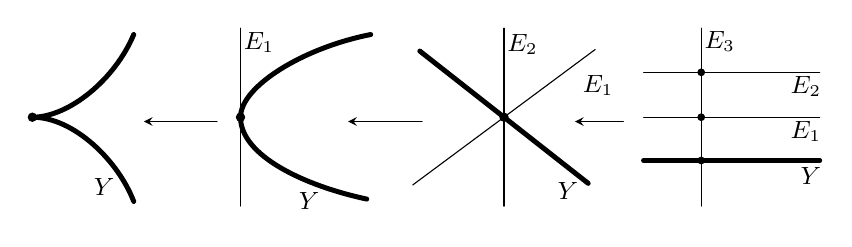
\begin{tikzpicture}[x=.99cm,y=1cm,>=stealth,line cap=round,font=\small]
\draw[line width=1.8pt] (1.3,1.05).. controls (1.06,.48) and (.47,0)..(0,0)
  .. controls (.53,0) and (1.1,-.55)..(1.3,-1.07);
\fill (0,0) circle[radius=1.7pt];\node at (.92,-.89) {$Y$};
\draw[<-] (1.43,-.055)--(2.37,-.055);
\draw (2.67,1.13)--(2.67,-1.13);
\draw[line width=1.8pt] (4.34,1.05).. controls (3.47,.88) and (2.67,.39)..(2.67,0)
  .. controls (2.67,-.49) and (3.49,-.87)..(4.29,-1.04);
\fill (2.67,0) circle[radius=1.7pt];
\node[above right,inner sep=1pt] at (2.67,.78) {$E_1$};
\node at (3.55,-1.06) {$Y$};
\draw[<-] (4.05,-.055)--(5,-.055);
\draw (6.05,1.13)--(6.05,-1.13);
\draw (4.88,-.86)--(7.22,.86);
\draw[line width=1.8pt] (4.97,.84)--(7.13,-.84);
\fill (6.05,0) circle[radius=1.7pt];
\node[above right,inner sep=1pt] at (6.05,.76) {$E_2$};
\node[below right,inner sep=1pt] at (7.02,.57) {$E_1$};
\node at (6.87,-.94) {$Y$};
\draw[<-] (6.96,-.055)--(7.58,-.055);
\draw (8.58,1.13)--(8.58,-1.13);
\draw (7.84,.57)--(10.1,.57) (7.84,0)--(10.1,0);
\draw[line width=1.8pt] (7.84,-.55)--(10.1,-.55);
\foreach \y in {.57,0,-.55}{\fill (8.58,\y) circle[radius=1.4pt];}
\node[above right,inner sep=1pt] at (8.58,.79) {$E_3$};
\node[below left,inner sep=1pt] at (10.16,.56) {$E_2$};
\node[below left,inner sep=1pt] at (10.16,-.01) {$E_1$};
\node[below left,inner sep=1pt] at (10.16,-.59) {$Y$};
\end{tikzpicture}\\[3pt]
\small\hypertarget{fig-book-20}{}Figure 20.\quad Embedded resolution of a cusp.
\end{center}

In the context of successive monoidal transformations, it is convenient to introduce the language of infinitely near points.

\Dfn Let $X$ be a surface. Then any point on any surface $X'$, obtained from $X$ by a finite succession of monoidal transformations, is called an \emph{infinitely near point} of $X$. If $g\colon X''\to X'$ is a further succession of monoidal transformations, and if $Q''\in X''$ is a point in the open set where $g$ is an isomorphism, then we identify $Q''$ with $g(Q'')$ as infinitely near points of $X$. In particular, all the ordinary points of $X$ are included among the infinitely near points. We say \textquotedblleft{}$Q$ is infinitely near $P$\textquotedblright{} if $P$ lies on some $X'$ and $Q$ lies on the exceptional curve $E$ obtained by blowing up $P$. If $C$ is a curve in $X$, and $Q'\in X'$ is an infinitely near point of $X$, we
}
% Contents from body/page-407.tex.
\ChapterSheet{407}{393}{\Goto{sec-V-3}{3\quad Monoidal Transformations}}{%
\noindent say $Q'$ is an \emph{infinitely near point} of $C$ if $Q'$ lies on the strict transform of $C$ on $X'$.

\medskip
\noindent\hypertarget{result-V-3.9.2}{}\textbf{Example 3.9.2.} Let $C$ be an irreducible curve on a surface $X$, with normalization $\widetilde C$. Then we have
\[
g(\widetilde C)=p_a(C)-\sum_P\tfrac12r_P(r_P-1),
\]
\noindent where $r_P$ is the multiplicity, and the sum is taken over all singular points $P$ of $C$, including infinitely near singular points. Indeed, by (\Goto{result-V-3.8}{3.8}) we pass from $C$ to $\widetilde C$ by blowing up the singular points in succession, until there are none left. Each time, by (\Goto{result-V-3.7}{3.7}), the arithmetic genus drops by $\frac12r(r-1)$.

\medskip
\noindent\hypertarget{result-V-3.9.3}{}\textbf{Example 3.9.3.} In particular, working with the infinitesimal neighborhood of one point at a time, we see that the integer $\delta_P$ of (IV, Ex.~\Goto{ex-IV-1.8}{1.8}) can be computed as $\sum\frac12r_Q(r_Q-1)$ taken over all infinitely near singular points $Q$ lying over $P$, including $P$.

\medskip
\noindent\hypertarget{result-V-3.9.4}{}\textbf{Remark 3.9.4} (Classification of Curve Singularities). With the ideas of this section we can begin a new classification of the possible singularities of a (reduced) curve lying on a surface, which is weaker than the classification by analytic isomorphism introduced in (I, \Goto{result-I-5.6.1}{5.6.1}) and (I, Ex.~\Goto{ex-I-5.14}{5.14})---see (Ex.~\Goto{ex-V-3.6}{3.6}). For references, see Walker [\Goto{bib-483-1}{1}, Ch.~III, \S7] and Zariski [\Goto{bib-zariski-10}{10}, Ch.~I].

As a first invariant of a singular point $P$ on a curve $C$ (lying always on a surface $X$) we have its multiplicity. Next we have the multiplicities of the infinitely near singular points of $C$, and their configuration around $P$. This data already suffices to determine $\delta_P$ (\Goto{result-V-3.9.3}{3.9.3}).

We define a slightly more complex, but still discrete, invariant of a singular point (or set of singular points), to be its equivalence class for the following equivalence relation. A (reduced) curve $C$ in an open set $U$ of a surface $X$ is \emph{equivalent} to another $C'\subseteq U'\subseteq X'$ if there is a sequence of monoidal transformations $U_n\to U_{n-1}\to\cdots\to U_0=U$ and another $U'_n\to U'_{n-1}\to\cdots\to U'_0=U'$, which give embedded resolutions for $C$ and $C'$ respectively, and if there is a one-to-one correspondence between the irreducible components of the reduced total transforms and their singular points at each step, preserving multiplicities, incidence, and compatible with the maps $U_i\to U_{i-1}$ and $U'_i\to U'_{i-1}$ for each $i$. One checks easily that this is in fact an equivalence relation. To define equivalence of a single singular point $P\in C$, just take $U$ so small that $C\cap U$ has no other singular points.

\medskip
\noindent\hypertarget{result-V-3.9.5}{}\textbf{Example 3.9.5.} To illustrate this concept, let us classify all double points up to equivalence. Let $P\in C$ be a double point, and let $\pi\colon\widetilde X\to X$ be the monoidal transformation with center $P$. Then as in the proof of (\Goto{result-V-3.9}{3.9}), there are three possibilities: (a) $\widetilde C$ meets $E$ transversally in two points, in which
}
% Contents from body/page-408.tex.
\ChapterSheet[10.9]{408}{394}{\Goto{p-370}{V\quad Surfaces}}{%
\noindent case $P$ is a node; (b) $\widetilde C$ meets $E$ in one point, and is tangent to it there, in which case $P$ is a cusp; (c) $\widetilde C$ is singular, with a double point $Q$. In this case $E$ must pass through $Q$ in a direction not equal to any tangent direction of $Q$, since $\widetilde C.E=2$. Therefore the equivalence class of $Q$ determines the equivalence class of $P$.

Thus we can classify double points according to the number of times $n$ we must blow up to get $\widetilde C$ nonsingular, and the behavior (a) or (b) at the last step.

\EditionText{Assume now that $\operatorname{char}k\ne2$. }In this case it happens that the classification for equivalence coincides with the classification for analytic isomorphism, although that is not true in general (Ex.~\Goto{ex-V-3.6}{3.6}). Indeed, up to analytic isomorphism, any double point is given by $y^2=x^r$ for some $r\ge2$ (I, Ex.~\Goto{ex-I-5.14}{5.14d}). To blow up, set $y=ux$. Then we get $u^2=x^{r-2}$. So we see inductively that the equivalence class is given by $n=\lfloor r/2\rfloor$ and the type is (a) if $r$ is even, (b) if $r$ is odd.

\Exercises
{\fontsize{9}{10.0}\selectfont\setlength{\parskip}{0pt}
\begin{description}[style=multiline,labelwidth=1.8em,leftmargin=2.15em,itemsep=3pt,topsep=0pt,parsep=0pt]
\item[\hypertarget{ex-V-3.1}{}3.1.] Let $X$ be a nonsingular projective variety of any dimension, let $Y$ be a \EditionText{proper nonsingular closed subvariety}, and let $\pi\colon\widetilde X\to X$ be obtained by blowing up $Y$. Show that $p_a(\widetilde X)=p_a(X)$.
\item[\hypertarget{ex-V-3.2}{}3.2.] Let $C$ and $D$ be curves on a surface $X$, meeting at a point $P$. Let $\pi\colon\widetilde X\to X$ be the monoidal transformation with center $P$. Show that $\widetilde C.\widetilde D=C.D-\mu_P(C)\cdot\mu_P(D)$. \EditionText{If $C$ and $D$ have no common irreducible component, conclude} that $C.D=\sum\mu_P(C)\cdot\mu_P(D)$, where the sum is taken over all intersection points of $C$ and $D$, including infinitely near intersection points.
\item[\hypertarget{ex-V-3.3}{}3.3.] Let $\pi\colon\widetilde X\to X$ be a monoidal transformation, and let $D$ be a very ample divisor on $X$. Show that $2\pi^*D-E$ is ample on $\widetilde X$. [\emph{Hint:} Use a suitable generalization of (I, Ex.~\Goto{ex-I-7.5}{7.5}) to curves in $\Proj^n$.]
\item[\hypertarget{ex-V-3.4}{}3.4.] \emph{Multiplicity of a Local Ring.} (See Nagata [\Goto{bib-480-14}{7}, Ch.~III, \S23] or Zariski--Samuel [\Goto{legacy-b-zs}{1}, vol.~2, Ch.~VIII, \S10].) Let $A$ be a noetherian local ring with maximal ideal $\mathfrak m$. For any $l>0$, let $\psi(l)=\operatorname{length}(A/\mathfrak m^l)$. We call $\psi$ the \emph{Hilbert--Samuel function} of $A$.
\begin{parts}
\item Show that there is a polynomial $P_A(z)\in\mathbf Q[z]$ such that $P_A(l)=\psi(l)$ for all $l\gg0$. This is the \emph{Hilbert--Samuel polynomial} of $A$. [\emph{Hint:} Consider the graded ring $\operatorname{gr}_{\mathfrak m}A=\bigoplus_{d\ge0}\mathfrak m^d/\mathfrak m^{d+1}$, and apply (I, \Goto{result-I-7.5}{7.5}).]
\item Show that $\deg P_A=\dim A$.
\item Let $n=\dim A$. Then we define the \emph{multiplicity} of $A$, denoted $\mu(A)$, to be $(n!)\cdot(\text{leading coefficient of }P_A)$. If $P$ is a point on a noetherian scheme $X$, we define the \emph{multiplicity of $P$ on $X$}, $\mu_P(X)$, to be $\mu(\mathcal O_{P,X})$.
\item Show that for a point $P$ on a curve $C$ on a surface $X$, this definition of $\mu_P(C)$ coincides with the one in the text just before (\Goto{result-V-3.5.2}{3.5.2}).
\item If $Y$ is a variety of degree $d$ in $\Proj^n$, show that the vertex of the cone over $Y$ is a point of multiplicity $d$.
\end{parts}
\item[\hypertarget{ex-V-3.5}{}3.5.] \EditionText{Assume $\operatorname{char}k\ne2$. }Let $a_1,\ldots,a_r$, $r\ge5$, be distinct elements of $k$, and let $C$ be the curve in $\Proj^2$ given by the (affine) equation $y^2=\prod_{i=1}^r(x-a_i)$. Show that the point $P$ at infinity on the $y$-axis is a singular point. Compute $\delta_P$ and \EditionText{$g(\widetilde C)$, where $\widetilde C$ is the normalization of $C$.} Show in this way that one obtains hyperelliptic curves of every genus $g\ge2$.
\end{description}
}
}
% Contents from body/page-409.tex.
\ChapterSheet{409}{395}{\Goto{sec-V-4}{4\quad The Cubic Surface in $\Proj^3$}}{%
{\fontsize{9}{10.4}\selectfont\setlength{\parskip}{0pt}
\begin{description}[style=multiline,labelwidth=1.8em,leftmargin=2.15em,itemsep=4pt,topsep=0pt,parsep=0pt]
\item[\hypertarget{ex-V-3.6}{}3.6.] Show that analytically isomorphic curve singularities (I, \Goto{result-I-5.6.1}{5.6.1}) are equivalent in the sense of (\Goto{result-V-3.9.4}{3.9.4}), but not conversely.
\item[\hypertarget{ex-V-3.7}{}3.7.] For each of the following singularities at $(0,0)$ in the plane, give an embedded resolution, compute $\delta_P$, and decide which ones are equivalent.
\begin{enumerate}[label=(\alph*),leftmargin=1.6em,itemsep=0pt,topsep=1pt]
\item $x^3+y^5=0$.
\item $x^3+x^4+y^5=0$.
\item $x^3+y^4+y^5=0$.
\item $x^3+y^5+y^6=0$.
\item $x^3+xy^3+y^5=0$.
\end{enumerate}
\item[\hypertarget{ex-V-3.8}{}3.8.] \EditionText{Show that the following two singularities have the same multiplicity at the origin. Compare their infinitely near multiplicities and compute the two distinct values of $\delta_P$. Show that the singularities are not equivalent.}
\begin{enumerate}[label=(\alph*),leftmargin=1.6em,itemsep=0pt,topsep=1pt]
\item $x^4-xy^4=0$.
\item $x^4-x^2y^3-x^2y^5+y^8=0$.
\end{enumerate}
\end{description}
}

\bigskip
\noindent\hypertarget{sec-V-4}{}\BookMark{1}{5.4  The Cubic Surface in \texorpdfstring{\ensuremath{\mathbf P^3}}{P3}}{sec-V-4}\textbf{\large 4\quad The Cubic Surface in $\Proj^3$}\par\medskip

\noindent In this section, as in \S\Goto{sec-V-2}{2}, we consider a very special class of surfaces, to illustrate some general principles. Our main result is that the projective plane with six points blown up is isomorphic to a nonsingular cubic surface in $\Proj^3$. We use this isomorphism to study the geometry of curves on the cubic surface. The isomorphism is accomplished using the linear system of plane cubic curves with six base points, so we begin with some general remarks about linear systems with base points.

Let $X$ be a surface, let $|D|$ be a complete linear system of curves on $X$, and let $P_1,\ldots,P_r$ be points of $X$. Then we will consider the sublinear system $\mathfrak d$ consisting of divisors $D\in|D|$ which pass through the points $P_1,\ldots,P_r$, and we denote it by $|D-P_1-\cdots-P_r|$. We say that $P_1,\ldots,P_r$ are the \emph{assigned base points} of $\mathfrak d$.

Let $\pi\colon X'\to X$ be the morphism obtained by blowing up $P_1,\ldots,P_r$, and let $E_1,\ldots,E_r$ be the exceptional curves. Then there is a natural one-to-one correspondence between the elements of $\mathfrak d$ on $X$ and the elements of the complete linear system $\mathfrak d'=|\pi^*D-E_1-\cdots-E_r|$ on $X'$ given by $D\mapsto\pi^*D-E_1-\cdots-E_r$, because the latter divisor is effective on $X'$ if and only if $D$ passes through $P_1,\ldots,P_r$.

The new linear system $\mathfrak d'$ on $X'$ may or may not have base points. We call any base point of $\mathfrak d'$ on $X'$, considered as an infinitely near point of $X$, an \emph{unassigned base point} of $\mathfrak d$.

These definitions also make sense if some of the $P_i$ themselves are infinitely near points of $X$, or if they are given with multiplicities greater than $1$. For example, if $P_2$ is infinitely near $P_1$, then for $D\in\mathfrak d$ we require that $D$ contain $P_1$, and that $\pi_1^*D-E_1$ contain $P_2$, where $\pi_1$ is the blowing-up of $P_1$. On the other hand, if $P_1$ is given with multiplicity $r\ge1$, then we require that $D$ have at least an $r$-fold point at $P_1$, and in the definition of $\mathfrak d'$, we take $\pi^*D-rE_1$.
}
% Contents from body/page-410.tex.
\ChapterSheet{410}{396}{\Goto{p-370}{V\quad Surfaces}}{%
(Note that if we assign base points $Q_1,\ldots,Q_s$ infinitely near a point $P$, then \EditionText{a divisor whose strict transform after blowing up $P$ contains these $s$ distinct points of the exceptional curve will have at least an $s$-fold point at $P$.} So we make the convention that every point $P$ must be assigned with a multiplicity at least equal to the sum of the multiplicities of the assigned base points infinitely near $P$.)

The usefulness of this language is that it gives us a way of talking about linear systems on various blown-up models of $X$, in terms of suitable linear systems with assigned base points on $X$.

\medskip
\noindent\hypertarget{result-V-4.0.1}{}\textbf{Remark 4.0.1.} Using this language, we can rephrase the condition (II, \Goto{result-II-7.8.2}{7.8.2}) for a complete linear system $|D|$ to be very ample as follows: $|D|$ is very ample if and only if (a) $|D|$ has no base points, and (b) for every $P\in X$, $|D-P|$ has no unassigned base points. Indeed, $|D|$ separates the points $P$ and $Q$ if and only if $Q$ is not a base point of $|D-P|$, and $|D|$ separates tangent vectors at $P$ if and only if $|D-P|$ has no unassigned base points infinitely near to $P$.

\medskip
\noindent\hypertarget{result-V-4.0.2}{}\textbf{Remark 4.0.2.} If we observe that the dimension drops by exactly one when we assign a base point which was not already an unassigned base point of a linear system, then we can rephrase this condition in a form reminiscent of (IV, \Goto{result-IV-3.1}{3.1}) as follows: $|D|$ is very ample if and only if for any two points $P,Q\in X$, including the case $Q$ infinitely near $P$,
\[
\dim|D-P-Q|=\dim|D|-2.
\]

\medskip
\noindent\hypertarget{result-V-4.0.3}{}\textbf{Remark 4.0.3.} Applying (\Goto{result-V-4.0.1}{4.0.1}) to a blown-up model of $X$, we see that if $\mathfrak d=|D-P_1-\cdots-P_r|$ is a linear system with assigned base points on $X$, then the associated linear system $\mathfrak d'$ on $X'$ is very ample on $X'$ if and only if (a) $\mathfrak d$ has no unassigned base points, and \EditionText{(b) for every $P\in X'$, viewed as an ordinary or infinitely near point of $X$, $\mathfrak d-P$ has no unassigned base points.}

\smallskip
Now we turn our attention to the particular situation of this section, which is linear systems of plane curves of fixed degree with assigned base points. We ask whether they have unassigned base points, and if not, we study the corresponding morphism of the blown-up model to a projective space. To get the cubic surface in $\Proj^3$ we will use the linear system of plane cubic curves with six base points. But first we need to consider linear systems of conics with base points. Here we use the word \emph{conic} (respectively, \emph{cubic}) to mean any effective divisor in the plane of degree $2$ (respectively, $3$).

\medskip
\noindent\hypertarget{result-V-4.1}{}\textbf{Proposition 4.1.} \emph{Let $\mathfrak d$ be the linear system of conics in $\Proj^2$ with assigned base points $P_1,\ldots,P_r$ and assume that no three of the $P_i$ are collinear. If $r\le4$, then $\mathfrak d$ has no unassigned base points. This result remains true if $P_2$ is infinitely near $P_1$.}
}
% Contents from body/page-411.tex.
\ChapterSheet{411}{397}{\Goto{sec-V-4}{4\quad The Cubic Surface in $\Proj^3$}}{%
\Proof Clearly it is sufficient to consider the case $r=4$. First suppose $P_1,P_2,P_3,P_4$ are all ordinary points. Let $L_{ij}$ denote the line containing $P_i$ and $P_j$. Then $\mathfrak d$ contains $L_{12}+L_{34}$ and $L_{13}+L_{24}$. Since no three of the $P_i$ are collinear, the intersection of these two divisors consists of the points $P_1,P_2,P_3,P_4$ with multiplicity $1$ each, so there are no unassigned base points.

Now suppose $P_2$ is infinitely near $P_1$. In this case $\mathfrak d$ contains $L_{12}+L_{34}$ and $L_{13}+L_{14}$. (Here, of course, $L_{12}$ denotes the line through $P_1$ with the tangent direction given by $P_2$.) This intersection again is just $\{P_1,P_2,P_3,P_4\}$, so there are no further base points.

\medskip
\noindent\hypertarget{result-V-4.2}{}\textbf{Corollary 4.2.} \emph{With the same hypotheses, we have:}
\begin{parts}
\item\hypertarget{result-V-4.2a}{} \emph{if $r\le5$, then $\dim\mathfrak d=5-r$;}
\item\hypertarget{result-V-4.2b}{} \emph{if $r=5$, then there exists a unique conic containing $P_1,\ldots,P_5$, which is necessarily irreducible.}
\end{parts}
\emph{Furthermore, these results remain true if $P_5$ is infinitely near any one of $P_1,\ldots,P_4$.}

\Proof\par
(\Goto{result-V-4.2a}{a}) Every time we prescribe a new base point on a linear system without unassigned base points, the dimension drops by one. Since the linear system of all conics in $\Proj^2$ has dimension $5$, this follows from (\Goto{result-V-4.1}{4.1}).

(\Goto{result-V-4.2b}{b}) For $r=5$, $\dim\mathfrak d=0$, so there is a unique conic containing $P_1,\ldots,P_5$. It must be irreducible since no three of the $P_i$ are collinear.

\medskip
\noindent\hypertarget{result-V-4.2.1}{}\textbf{Remark 4.2.1.} This last statement is the classical result that a conic is uniquely determined by giving $5$ points, or $4$ points and a tangent direction at one of them, or $3$ points with tangent directions at two of them, or even $3$ points with a tangent direction and a second order tangent direction at one of them (when $P_5$ is infinitely near $P_2$ which is infinitely near $P_1$).

\medskip
\noindent\hypertarget{result-V-4.2.2}{}\textbf{Example 4.2.2.} If $r=1$, then $\mathfrak d$ has no unassigned base points, and for any point $P$, $\mathfrak d-P$ has no unassigned base points, so by (\Goto{result-V-4.0.3}{4.0.3}), $\mathfrak d'$ is very ample on $X'$. Since $\dim\mathfrak d'=4$, it gives an embedding of $X'$ in $\Proj^4$, as a surface of degree $3$, which is the number of unassigned intersection points of two divisors in $\mathfrak d$. In fact, $X'$ is just the rational ruled surface with $e=1$, and this embedding is the rational cubic scroll (\Goto{result-V-2.19.1}{2.19.1}).

\medskip
\noindent\hypertarget{result-V-4.2.3}{}\textbf{Example 4.2.3.} If $r=3$, then $X'$ is $\Proj^2$ with three points blown up, and $\dim\mathfrak d=2$. Since $\mathfrak d'$ has no base points, it determines a morphism $\psi$ of $X'$ to $\Proj^2$. We may take the three points to be $P_1=(1,0,0)$, $P_2=(0,1,0)$ and $P_3=(0,0,1)$. Then the vector space $V\subseteq H^0(\mathcal O_{\Proj^2}(2))$ corresponding to $\mathfrak d$ is spanned by $x_1x_2$, $x_0x_2$, and $x_0x_1$, so $\psi$ can be defined by $y_0=x_1x_2$, $y_1=x_0x_2$, $y_2=x_0x_1$, where $y_i$ are the homogeneous coordinates of the new $\Proj^2$. Considered as a rational map from $\Proj^2$ to $\Proj^2$, this is none other than the \emph{quadratic transformation} $\varphi$ of (I, Ex.~\Goto{ex-I-4.6}{4.6}).
}
% Contents from body/page-412.tex.
\ChapterSheet[10.7]{412}{398}{\Goto{p-370}{V\quad Surfaces}}{%
Now we will show that $\psi$ identifies $X'$ with the second $\Proj^2$, blown up at the points $Q_1=(1,0,0)$, $Q_2=(0,1,0)$, and $Q_3=(0,0,1)$, in such a way that the exceptional curve $\psi^{-1}(Q_i)$ is the strict transform of the line $L_{jk}$ joining $P_j,P_k$ on the first $\Proj^2$, for each $(i,j,k)=(1,2,3)$ in some order. Furthermore $\psi(E_i)$ is the line $M_{jk}$ joining $Q_j$ and $Q_k$, for each $(i,j,k)=(1,2,3)$. Thus we can say that the quadratic transformation $\varphi$ is just \textquotedblleft{}blowing up the points $P_1,P_2,P_3$ and blowing down the lines $\widetilde L_{12},\widetilde L_{13},\widetilde L_{23}$\textquotedblright{} (Fig.~\Goto{fig-book-21}{21}).

\begin{center}
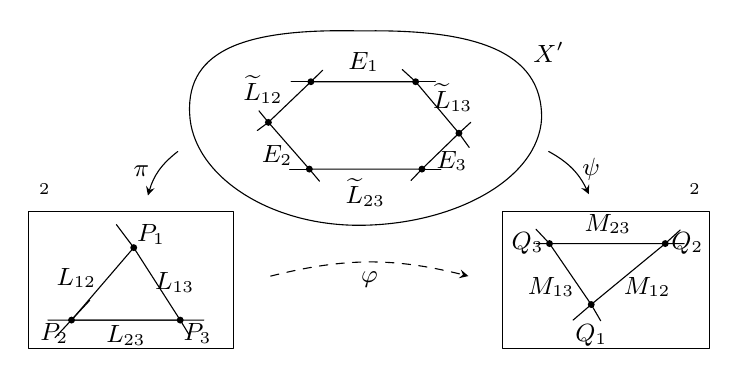
\begin{tikzpicture}[x=1cm,y=.86cm,>=stealth,line cap=round,line join=round,font=\small]
\draw (0,1.47) .. controls (1.42,1.5) and (2.31,1.19) .. (2.3,.18)
  .. controls (2.26,-.72) and (1.19,-1.39) .. (0,-1.4)
  .. controls (-1.17,-1.41) and (-2.14,-.65) .. (-2.17,.25)
  .. controls (-2.21,1.21) and (-1.43,1.51) .. (0,1.47);
\node at (2.39,1.15) {$X'$};
\coordinate (a) at (-.63,.72);\coordinate (b) at (.7,.72);
\coordinate (c) at (1.25,-.04);\coordinate (d) at (.78,-.57);
\coordinate (e) at (-.65,-.57);\coordinate (f) at (-1.17,.12);
\draw (a)--(b)--(c)--(d)--(e)--(f)--cycle;
\draw (-.88,.72)--(-.63,.72) (.7,.72)--(.95,.72)
      (-.9,-.57)--(-.65,-.57) (.78,-.57)--(1.02,-.57);
\draw (-1.31,0)--(-1.17,.12) (-.63,.72)--(-.48,.89)
      (.53,.9)--(.7,.72) (1.25,-.04)--(1.38,-.25)
      (-1.29,.29)--(-1.17,.12) (-.65,-.57)--(-.52,-.75)
      (.64,-.74)--(.78,-.57) (1.25,-.04)--(1.4,.12);
\foreach \v in {a,b,c,d,e,f}{\fill (\v) circle[radius=1.25pt];}
\node[above] at (.04,.72) {$E_1$};
\node at (-1.24,.61) {$\widetilde L_{12}$};
\node at (1.17,.49) {$\widetilde L_{13}$};
\node at (-1.06,-.37) {$E_2$};
\node at (1.16,-.45) {$E_3$};
\node[below] at (.06,-.57) {$\widetilde L_{23}$};
\draw (-4.22,-1.19) rectangle (-1.61,-3.22);
\node[above right,inner sep=2pt] at (-4.16,-1.19) {$\Proj^2$};
\coordinate (p1) at (-2.88,-1.73);
\coordinate (p2) at (-3.67,-2.8);
\coordinate (p3) at (-2.29,-2.8);
\draw (p1)--(p2)--(p3)--cycle;
\draw (-3.1,-1.39)--(p1) (-3.44,-2.51)--(-3.88,-3.06)
      (p3)--(-2.18,-3.01) (-3.97,-2.8)--(-1.99,-2.8);
\foreach \v in {p1,p2,p3}{\fill (\v) circle[radius=1.25pt];}
\node[above right,inner sep=1pt] at (p1) {$P_1$};
\node[below left,inner sep=1pt] at (p2) {$P_2$};
\node[below right,inner sep=1pt] at (p3) {$P_3$};
\node at (-3.61,-2.18) {$L_{12}$};
\node at (-2.36,-2.25) {$L_{13}$};
\node at (-2.98,-3.03) {$L_{23}$};
\draw (1.8,-1.19) rectangle (4.43,-3.22);
\node[above left,inner sep=2pt] at (4.4,-1.19) {$\Proj^2$};
\coordinate (q3) at (2.4,-1.67);
\coordinate (q2) at (3.87,-1.67);
\coordinate (q1) at (2.93,-2.57);
\draw (q3)--(q2)--(q1)--cycle;
\draw (2.23,-1.67)--(q3) (q2)--(4.11,-1.67)
      (2.23,-1.46)--(q3) (q1)--(3.05,-2.81)
      (q2)--(4.06,-1.47) (q1)--(2.7,-2.8);
\foreach \v in {q1,q2,q3}{\fill (\v) circle[radius=1.25pt];}
\node[left,inner sep=2pt] at (q3) {$Q_3$};
\node[right,inner sep=2pt] at (q2) {$Q_2$};
\node[below,inner sep=1pt] at (2.93,-2.82) {$Q_1$};
\node at (2.42,-2.31) {$M_{13}$};
\node at (3.64,-2.31) {$M_{12}$};
\node[above] at (3.14,-1.67) {$M_{23}$};
\draw[->] (-2.32,-.31) to[bend right=18] node[left] {$\pi$} (-2.7,-.96);
\draw[->] (2.39,-.31) to[bend left=18] node[right] {$\psi$} (2.9,-.94);
\draw[->,dashed] (-1.14,-2.15) to[bend left=14] node[below] {$\varphi$} (1.37,-2.15);
\end{tikzpicture}\\[3pt]
\small\hypertarget{fig-book-21}{}Figure 21.\quad The quadratic transformation of $\Proj^2$.
\end{center}

To prove this, we consider the variety $V$ in $\Proj^2\times\Proj^2$ defined by the bihomogeneous equations $x_0y_0=x_1y_1=x_2y_2$. I claim the first projection $p_1\colon V\to\Proj^2$ identifies $V$ with $X'$. This is a local question, since blowing up a point depends only on the neighborhood of the point, so we consider the open set $U\subseteq\Proj^2$ defined by $x_0=1$. Then $U=\operatorname{Spec}A$ with $A=k[x_1,x_2]$, and $p_1^{-1}(U)$ can be written as
\[
p_1^{-1}(U)=\operatorname{Proj} A[y_0,y_1,y_2]/(y_0-x_1y_1,x_1y_1-x_2y_2).
\]
\noindent We can eliminate $y_0$ from the graded ring, so
\[
p_1^{-1}(U)\cong\operatorname{Proj} A[y_1,y_2]/(x_1y_1-x_2y_2).
\]
\noindent But this shows that $p_1^{-1}(U)$ is isomorphic to $U$ with the point $(x_1,x_2)=(0,0)$ blown up, as in the proof of (\Goto{result-V-3.6}{3.6}).

Doing the same with the open sets $x_1=1$ and $x_2=1$ of $\Proj^2$, we see that $V$, via the first projection, is just $\Proj^2$ with the points $P_1,P_2,P_3$ blown up, so $V\cong X'$. By symmetry, $V$ with the second projection is the second $\Proj^2$ with the points $Q_1,Q_2,Q_3$ blown up. So $p_2\circ p_1^{-1}$ gives a birational transformation of $\Proj^2$ to itself. Solving the equations $x_0y_0=x_1y_1=x_2y_2$ in the case $x_0,x_1,x_2\ne0$, we get $y_0=x_1x_2$, $y_1=x_0x_2$, $y_2=x_0x_1$, so that this transformation is again the quadratic transformation $\varphi$ above.

We conclude that $\psi\colon X'\to\Proj^2$ is the same as $p_2\colon V\to\Proj^2$, so that $\varphi$ is just blowing up three points and blowing down three lines. Finally, it is clear from the equations that $p_2(\widetilde L_{ij})=Q_k$ and $p_2(E_i)=M_{jk}$ for each $i,j,k$.
}
% Contents from body/page-413.tex.
\ChapterSheet{413}{399}{\Goto{sec-V-4}{4\quad The Cubic Surface in $\Proj^3$}}{%
\noindent\hypertarget{result-V-4.3}{}\textbf{Proposition 4.3.} \emph{Let $\mathfrak d$ be the linear system of plane cubic curves with assigned base points $P_1,\ldots,P_r$, and assume that no $4$ of the $P_i$ are collinear, and no $7$ of them lie on a conic. If $r\le7$, then $\mathfrak d$ has no unassigned base points. This result remains true if $P_2$ is infinitely near $P_1$.}

\Proof It is sufficient to consider the case $r=7$. We will show first that if $P_1,\ldots,P_7$ are all ordinary points, then $\mathfrak d$ has no unassigned ordinary base points. For this it is sufficient to exhibit, for each point $Q$ not equal to any $P_i$, a cubic curve containing $P_1,\ldots,P_7$ but not $Q$.

\emph{Case 1.} Suppose there exist some three points $P_1,P_2,P_3$ lying on a line $L^*$ with $Q$. The points $P_4,P_5,P_6,P_7$ are not all collinear, so we may assume that $P_4,P_5,P_6$ are not collinear. Then the conic $\Gamma_{12456}$ through $P_1,P_2,P_4,P_5,P_6$, together with the line $L_{37}$ through $P_3$ and $P_7$ forms a cubic curve containing $P_1,\ldots,P_7$ but not $Q$. Indeed, if $Q\in\Gamma_{12456}$, then this conic contains the line $L^*$, so it is reducible, in which case $P_4,P_5,P_6$ must be collinear, which is a contradiction. If $Q\in L_{37}$, then $P_7\in L^*$, so $P_1,P_2,P_3,P_7$ are collinear, which is a contradiction.

\emph{Case 2.} Suppose that $Q$ is not collinear with any set of three of the points $P_i$, but that $Q$ lies on a conic $\Gamma^*$ (necessarily irreducible) containing $6$ of them, say $P_1,\ldots,P_6$. Then $\Gamma_{12347}+L_{56}$ is a cubic not containing $Q$. Indeed, if $Q\in\Gamma_{12347}$, then $P_1,P_2,P_3,P_4,Q$ are in this conic and also in $\Gamma^*$, so by (\Goto{result-V-4.2}{4.2}), $\Gamma_{12347}=\Gamma^*$. But then $P_1,\ldots,P_7$ are all in $\Gamma^*$, a contradiction. If $Q\in L_{56}$, then $\Gamma^*$ is reducible, a contradiction.

\emph{Case 3.} $Q$ is not collinear with any $3$ of the $P_i$, and not on a conic with any $6$ of them. Then consider the three cubic curves $C_i=\Gamma_{1234i}+L_{jk}$, where $(i,j,k)=(5,6,7)$ in some order. We will show that one of these does not contain $Q$. If $Q\in L_{56}$, then $Q\notin L_{57}$ and $Q\notin L_{67}$, because in either case $P_5,P_6,P_7,Q$ would be collinear. So, ruling out $C_7$, we may assume $Q\notin L_{57}$ and $Q\notin L_{67}$. Then, if $Q\in C_5$ and $Q\in C_6$, we have $Q\in\Gamma_{12345}$ and $Q\in\Gamma_{12346}$. Consider the conic $\Gamma'=\Gamma_{1234Q}$. If $\Gamma'$ is irreducible, then from (\Goto{result-V-4.2}{4.2}) we have all three conics equal, so $Q\in\Gamma_{123456}$, which is a contradiction. If $\Gamma'$ is reducible, then for a suitable relabeling, we have either (a) $\Gamma'=L_{123}+L_{4Q}$ or (b) $\Gamma'=L_{12Q}+L_{34}$. In case (a), $\Gamma_{12345}=L_{123}+L_{45}$ and $\Gamma_{12346}=L_{123}+L_{46}$, so $P_4,P_5,P_6$ and $Q$ are collinear, a contradiction. In case (b), $\Gamma_{12345}=L_{12}+L_{345}$ and $\Gamma_{12346}=L_{12}+L_{346}$, so $P_3,P_4,P_5,P_6$ are collinear, a contradiction.

This completes the proof in the case $P_1,\ldots,P_7$ and $Q$ are all ordinary points. The same proof also works in case $P_2$ is infinitely near $P_1$, or $Q$ is infinitely near one of $P_1,\ldots,P_7$, or both. One has to relabel the $P_i$ occasionally so that the constructions make sense, and one has to use (\Goto{result-V-4.2}{4.2}) in the case of infinitely near points also. (Details left to reader.)

\medskip
\noindent\hypertarget{result-V-4.4}{}\textbf{Corollary 4.4.} \emph{With the same hypotheses, we have}
\begin{parts}
\item\hypertarget{result-V-4.4a}{} \emph{if $r\le8$, then $\dim\mathfrak d=9-r$, and}
\item\hypertarget{result-V-4.4b}{} \emph{if $r=8$, $\dim\mathfrak d=1$ and almost every curve in $\mathfrak d$ is irreducible.}
\end{parts}
}
% Contents from body/page-414.tex.
\ChapterSheet{414}{400}{\Goto{p-370}{V\quad Surfaces}}{%
\noindent\textsc{Proof.} For $r\le7$ there are no unassigned base points, so at each step, the dimension drops by one. The cubics with no base points form a linear system of dimension $9$. This proves (a). To prove (b), we observe that with no $4$ points collinear and no $7$ on a conic, there are only finitely many ways of passing three lines, or one line and one irreducible conic through the $8$ points.

\medskip
\noindent\hypertarget{result-V-4.5}{}\textbf{Corollary 4.5.} \emph{Given $8$ points $P_1,\dots,P_8$ in the plane, no $4$ collinear, and no $7$ lying on a conic, there is a uniquely determined point $P_9$ (possibly an infinitely near point) such that every cubic through $P_1,\dots,P_8$ also passes through $P_9$. This is still true if $P_2$ is infinitely near $P_1$, and $P_8$ is infinitely near any one of $P_1,\dots,P_7$.}

\smallskip
\noindent\textsc{Proof.} By (\Goto{result-V-4.4}{4.4}) the linear system $\mathfrak d$ of all cubics through $P_1,\dots,P_8$ has dimension one, and we can choose two distinct irreducible ones $C,C'\in\mathfrak d$. Then by B\'ezout's theorem (\Goto{result-V-1.4.2}{1.4.2}) (cf.\ Ex.~\Goto{ex-V-3.2}{3.2}), $C$ and $C'$ meet in $9$ points, $8$ of which are $P_1,\dots,P_8$. So this determines a ninth point $P_9$, possibly an infinitely near point. Now since $\dim\mathfrak d=1$, any other curve $C''\in\mathfrak d$, irreducible or not, is a linear combination of $C$ and $C'$, so it must also pass through $P_9$. Thus $P_9$ is an unassigned base point of $\mathfrak d$.

\medskip
\noindent\hypertarget{result-V-4.5.1}{}\textbf{Remark 4.5.1.} This classical result has a number of interesting geometrical consequences. See (Ex.~\Goto{ex-V-4.4}{4.4}), (Ex.~\Goto{ex-V-4.5}{4.5}).

\medskip
\noindent\hypertarget{result-V-4.6}{}\textbf{Theorem 4.6.} \emph{Let $\mathfrak d$ be the linear system of plane cubic curves with assigned (ordinary) base points $P_1,\dots,P_r$, and assume that no $3$ of the $P_i$ are collinear, and no $6$ of them lie on a conic. If $r\le6$, then the corresponding linear system $\mathfrak d'$ on the surface $X'$ obtained from $\mathbf P^2$ by blowing up $P_1,\dots,P_r$, is very ample.}

\smallskip
\noindent\textsc{Proof.} According to (\Goto{result-V-4.0.3}{4.0.3}) we must verify that $\mathfrak d$ has no unassigned base points, and that for every point $P$, possibly infinitely near, $\mathfrak d-P$ has no unassigned base points. The first statement is an immediate consequence of (\Goto{result-V-4.3}{4.3}). For the second, we note that since no $3$ of the $P_i$ are collinear, and no $6$ of them lie on a conic, the $r+1$ points $P_1,\dots,P_r,P$ satisfy the hypotheses of (\Goto{result-V-4.3}{4.3}). So this case also follows from (\Goto{result-V-4.3}{4.3}).

\medskip
\noindent\hypertarget{result-V-4.7}{}\textbf{Corollary 4.7.} \emph{With the same hypotheses, for each $r=0,1,\dots,6$, we obtain an embedding of $X'$ in $\mathbf P^{9-r}$ as a surface of degree $9-r$, whose canonical sheaf $\omega_{X'}$ is isomorphic to $\mathcal O_{X'}(-1)$. In particular, for $r=6$, we obtain a nonsingular cubic surface in $\mathbf P^3$.}

\smallskip
\noindent\textsc{Proof.} We embed $X'$ in $\mathbf P^N$ via the very ample linear system $\mathfrak d'$. Since $\dim\mathfrak d=\dim\mathfrak d'=9-r$ by (\Goto{result-V-4.4}{4.4}), we have $N=9-r$. If $L$ is a line in $\mathbf P^2$, then $\mathfrak d'=|\pi^*3L-E_1-\dots-E_r|$, so for any $D'\in\mathfrak d'$, we have $D'^2=9-r$. Therefore the degree of $X'$ in $\mathbf P^N$ is $9-r$. Finally, since the canonical divisor on $\mathbf P^2$ is $-3L$, we see from (\Goto{result-V-3.3}{3.3}) that $K_{X'}=-\pi^*3L+E_1+\dots+{}$}
% Contents from body/page-415.tex.
\ChapterSheet[10.45]{415}{401}{\Goto{sec-V-4}{4\quad The Cubic Surface in $\mathbf P^3$}}{%
\noindent $E_r$, which is just $-D'$. Therefore $\omega_{X'}\cong\mathcal O_{X'}(-1)$ in the given projective embedding.

\medskip
\noindent\hypertarget{result-V-4.7.1}{}\textbf{Remark 4.7.1.} A \emph{Del Pezzo surface} is defined to be a surface $X$ of degree $d$ in $\mathbf P^d$ such that $\omega_X\cong\mathcal O_X(-1)$. So (\Goto{result-V-4.7}{4.7}) gives a construction of Del Pezzo surfaces of degrees $d=3,4,\dots,9$. A classical result states that every Del Pezzo surface is either one given by (\Goto{result-V-4.7}{4.7}) for a suitable choice of points $P_i\in\mathbf P^2$, or the $2$-uple embedding of a quadric surface in $\mathbf P^3$, which is a Del Pezzo surface of degree $8$ in $\mathbf P^8$. In particular, every nonsingular cubic surface in $\mathbf P^3$ can be obtained by blowing up $6$ points in the plane. Indeed, for a cubic surface in $\mathbf P^3$, the condition $\omega_X\cong\mathcal O_X(-1)$ is automatic (II, Ex.~\Goto{ex-II-8.4}{8.4}). For proofs see, e.g., Manin \Goto{bib-479-14}{[3, \S24]} or Nagata \Goto{bib-nagata-5}{[5, I, Thm.~8, p.~366]}.

\medskip
\noindent\hypertarget{result-V-4.7.2}{}\textbf{Remark 4.7.2.} In the case of cubic surfaces in $\mathbf P^3$, we can prove a slightly weaker result by counting constants. The choice of $6$ points in the plane requires $12$ parameters. \EditionText{Choosing a projective frame adds $15$ parameters. For a fixed embedded cubic surface there are only finitely many ordered sets of six exceptional lines by (\Goto{result-V-4.9}{4.9}). For each such set, $3l=h+\sum e_i$ determines $l$ in the torsion-free Picard group, and $|l|$ determines the contraction up to the $8$ parameters for coordinates on $\mathbf P^2$. Consequently the image has dimension $12+15-8=19$. It contains a nonempty open set in the irreducible $19$-dimensional space of cubic surfaces.}

\medskip
\noindent\hypertarget{result-V-4.7.3}{}\textbf{Notation 4.7.3.} For the rest of this section, we specialize to the case of the cubic surface in $\mathbf P^3$, and fix our notation. Let $P_1,\dots,P_6$ be six points of the plane, no three collinear, and not all six lying on a conic. Let $\mathfrak d$ be the linear system of plane cubic curves through $P_1,\dots,P_6$, and let $X$ be the nonsingular cubic surface in $\mathbf P^3$ obtained by (\Goto{result-V-4.7}{4.7}). Thus $X$ is isomorphic to $\mathbf P^2$ with the six points $P_1,\dots,P_6$ blown up. Let $\pi\colon X\to\mathbf P^2$ be the projection. Let $E_1,\dots,E_6\subseteq X$ be the exceptional curves, and let $e_1,\dots,e_6\in\operatorname{Pic}X$ be their linear equivalence classes. Let $l\in\operatorname{Pic}X$ be the class of $\pi^*$ of a line in $\mathbf P^2$.

\medskip
\noindent\hypertarget{result-V-4.8}{}\textbf{Proposition 4.8.} {\itshape Let $X$ be the cubic surface in $\mathbf P^3$ (\Goto{result-V-4.7.3}{4.7.3}). Then:

\hspace*{1.5em}(a) $\operatorname{Pic}X\cong\mathbb Z^7$, generated by $l,e_1,\dots,e_6$;

\hspace*{1.5em}(b) the intersection pairing on $X$ is given by $l^2=1$, $e_i^2=-1$, $l\cdot e_i=0$, $e_i\cdot e_j=0$ for $i\ne j$;

\hspace*{1.5em}(c) the hyperplane section $h$ is $3l-\sum e_i$;

\hspace*{1.5em}(d) the canonical class is $K=-h=-3l+\sum e_i$;

\hspace*{1.5em}(e) if $D$ is any effective divisor on $X$, $D\sim al-\sum b_ie_i$, then the degree of $D$, as a curve in $\mathbf P^3$, is
\[
d=3a-\sum b_i;
\]
\hspace*{1.5em}(f) the self-intersection of $D$ is $D^2=a^2-\sum b_i^2$;

\hspace*{1.5em}(g) the arithmetic genus of $D$ is
\[
p_a(D)=\frac12(D^2-d)+1=\frac12(a-1)(a-2)-\frac12\sum b_i(b_i-1).
\]}}
% Contents from body/page-416.tex.
\ChapterSheet[10.55]{416}{402}{\Goto{p-370}{V\quad Surfaces}}{%
\noindent\textsc{Proof.} All of this follows from earlier results. (a) and (b) follow from (\Goto{result-V-3.2}{3.2}). (c) comes from the definition of the embedding in $\mathbf P^3$. (d) comes from (\Goto{result-V-3.3}{3.3}). For (e), we note that the degree of $D$ is just $D\cdot h$. (f) is immediate from (b), and (g) follows from the adjunction formula $2p_a(D)-2=D\cdot(D+K)$ (Ex.~\Goto{ex-V-1.3}{1.3}) and the fact that $D\cdot K=-D\cdot h=-d$ by (d).

\medskip
\noindent\hypertarget{result-V-4.8.1}{}\textbf{Remark 4.8.1.} If $C$ is any irreducible curve in $X$, other than $E_1,\dots,E_6$, then $\pi(C)$ is an irreducible plane curve $C_0$, and $C$ in turn is the strict transform of $C_0$. Let $C_0$ have degree $a$, and suppose that $C_0$ has a point of multiplicity $b_i$ at each $P_i$. Then $\pi^*C_0=C+\sum b_iE_i$, by (\Goto{result-V-3.6}{3.6}). Since $C_0\sim a\cdot\text{line}$, we conclude that $C\sim al-\sum b_ie_i$. Thus for any $a,b_1,\dots,b_6\ge0$, we can interpret an irreducible curve $C$ on $X$ in the class $al-\sum b_ie_i$ as the strict transform of a plane curve of degree $a$ with a $b_i$-fold point at each $P_i$. So the study of curves on $X$ is reduced to the study of certain plane curves.

\medskip
\noindent\hypertarget{result-V-4.9}{}\textbf{Theorem 4.9} (Twenty-Seven Lines). {\itshape The cubic surface $X$ contains exactly $27$ lines. Each one has self-intersection $-1$, and they are the only irreducible curves with negative self-intersection on $X$. They are

\hspace*{1.5em}(a) the exceptional curves $E_i$, $i=1,\dots,6$ (six of these),

\hspace*{1.5em}(b) the strict transform $F_{ij}$ of the line in $\mathbf P^2$ containing $P_i$ and $P_j$, $1\le i<j\le6$ (fifteen of these), and

\hspace*{1.5em}(c) the strict transform $G_j$ of the conic in $\mathbf P^2$ containing the five $P_i$ for $i\ne j$, $j=1,\dots,6$ (six of these).}

\smallskip
\noindent\textsc{Proof.} First of all, if $L$ is any line in $X$, then $\deg L=1$ and $p_a(L)=0$, so by (\Goto{result-V-4.8}{4.8}) we have $L^2=-1$. (See also (Ex.~\Goto{ex-V-1.4}{1.4}).) Conversely, if $C$ is an irreducible curve on $X$ with $C^2<0$, then since $p_a(C)\ge0$, we must have $C^2=-1$, $p_a(C)=0$, $\deg C=1$ again by (\Goto{result-V-4.8}{4.8}), so $C$ is a line.

Next, from (\Goto{result-V-4.8.1}{4.8.1}) we see that $E_i\sim e_i$, $F_{ij}\sim l-e_i-e_j$, and $G_j\sim 2l-\sum_{i\ne j}e_i$, and we see immediately from (\Goto{result-V-4.8}{4.8}) that each of these has degree $1$, i.e., is a line.

It remains to show that if $C$ is any irreducible curve on $X$ with $\deg C=1$ and $C^2=-1$, then $C$ is one of those $27$ lines listed. Assuming $C$ is not one of the $E_i$, we can write $C\sim al-\sum b_ie_i$, and by (\Goto{result-V-4.8.1}{4.8.1}) we must have $a>0$, $b_i\ge0$. Furthermore,
\[
\begin{aligned}
\deg C&=3a-\sum b_i=1\\
C^2&=a^2-\sum b_i^2=-1.
\end{aligned}
\]
We will show that the only integers $a,b_1,\dots,b_6$ satisfying all these conditions are those corresponding to the $F_{ij}$ and $G_j$ above.

Recall Schwarz's inequality, which says that if $x_1,x_2,\dots,y_1,y_2,\dots$ are two sequences of real numbers, then
\[
\bigl|\sum x_iy_i\bigr|^2\le\bigl|\sum x_i^2\bigr|\cdot\bigl|\sum y_i^2\bigr|.
\]
Taking $x_i=1$, $y_i=b_i$, $i=1,\dots,6$, we find
\[
(\sum b_i)^2\le6(\sum b_i^2).
\]}
% Contents from body/page-417.tex.
\ChapterSheet[10.55]{417}{403}{\Goto{sec-V-4}{4\quad The Cubic Surface in $\mathbf P^3$}}{%
\noindent Substituting $\sum b_i=3a-1$ and $\sum b_i^2=a^2+1$ from above, we obtain
\[
3a^2-6a-5\le0.
\]
Solving the quadratic equation, this implies $a\le1+(2/3)\sqrt6<3$. Therefore $a=1$ or $2$. Now one quickly finds all possible values of the $b_i$ by trial: if $a=1$, then $b_i=b_j=1$ for some $i,j$, the rest $0$. This gives $F_{ij}$. If $a=2$, then all $b_i=1$ except for one $b_j=0$. This gives $G_j$.

\medskip
\noindent\hypertarget{result-V-4.9.1}{}\textbf{Remark 4.9.1.} There is lots of classical projective geometry associated with the $27$ lines. For example, the configuration of $12$ lines $E_1,\dots,E_6,G_1,\dots,G_6$ in $\mathbf P^3$ with the property that the $E_i$ are mutually skew, the $G_j$ are mutually skew, and $E_i$ meets $G_j$ if and only if $i\ne j$, is called \emph{Schl\"afli's double-six}. One can show that given a line $E_1$, and five lines $G_2,\dots,G_6$ meeting it, but otherwise in sufficiently general position, then other lines $E_2,\dots,E_6$ and $G_1$ are uniquely determined so as to form a double-six. Furthermore, each double-six is contained in a unique nonsingular cubic surface, and thus forms part of a set of $27$ lines on a cubic surface. See Hilbert and Cohn-Vossen \Goto{bib-477-10-item-1}{[1, \S25]}. The $27$ lines have a high degree of symmetry, as we see in the next result.

\medskip
\noindent\hypertarget{result-V-4.10}{}\textbf{Proposition 4.10.} \emph{Let $X$ be a cubic surface as above, and let $E'_1,\dots,E'_6$ be any subset of six mutually skew lines chosen from among the $27$ lines on $X$. Then there is another morphism $\pi'\colon X\to\mathbf P^2$, making $X$ isomorphic to that $\mathbf P^2$ with six points $P'_1,\dots,P'_6$ blown up (no $3$ collinear and not all $6$ on a conic), such that $E'_1,\dots,E'_6$ are the exceptional curves for $\pi'$.}

\smallskip
\noindent\textsc{Proof.} We proceed stepwise, working with one line at a time. We will show first that it is possible to find $\pi'$ such that $E'_1$ is the inverse image of $P'_1$.

\emph{Case 1.} If $E'_1$ is one of the $E_i$, we take $\pi'=\pi$, but relabel the $P_i$ so that $P_i$ becomes $P'_1$.

\emph{Case 2.} If $E'_1$ is one of the $F_{ij}$, say $E'_1=F_{12}$, then we apply the quadratic transformation with centers $P_1,P_2,P_3$ (\Goto{result-V-4.2.3}{4.2.3}) as follows. Let $X_0$ be $\mathbf P^2$ with $P_1,P_2,P_3$ blown up, let $\pi_0\colon X_0\to\mathbf P^2$ be the projection, and let $\psi\colon X_0\to\mathbf P^2$ be the other map to $\mathbf P^2$ of (\Goto{result-V-4.2.3}{4.2.3}), so that $X_0$ via $\psi$ is $\mathbf P^2$ with $Q_1,Q_2,Q_3$ blown up. Since $\pi\colon X\to\mathbf P^2$ expresses $X$ as $\mathbf P^2$ with $P_1,\dots,P_6$ blown up, $\pi$ factors through $\pi_0$, say $\pi=\pi_0\circ\theta$, where $\theta\colon X\to X_0$. Now we define $\pi'$ as $\psi\circ\theta$.
\[
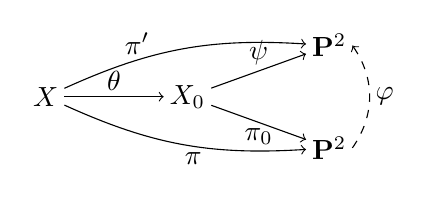
\begin{tikzpicture}[baseline=(x.base),every node/.style={inner sep=2pt}]
\node (x) at (0,0) {$X$};
\node (x0) at (1.8,0) {$X_0$};
\node (p1) at (3.6,.65) {$\mathbf P^2$};
\node (p2) at (3.6,-.65) {$\mathbf P^2$};
\draw[->] (x) -- node[above] {$\theta$} (x0);
\draw[->] (x0) -- node[above] {$\psi$} (p1);
\draw[->] (x0) -- node[below] {$\pi_0$} (p2);
\draw[->] (x) to[bend left=14] node[above,pos=.3] {$\pi'$} (p1);
\draw[->] (x) to[bend right=14] node[below,pos=.55] {$\pi$} (p2);
\draw[dashed,->] (p2.east) to[bend right=35] node[right] {$\varphi$} (p1.east);
\end{tikzpicture}
\]
Then, using the notation of (\Goto{result-V-4.2.3}{4.2.3}), $\theta(F_{12})=\widetilde L_{12}$, so $\pi'(F_{12})=Q_3$. Furthermore, $\pi'$ expresses $X$ as $\mathbf P^2$ with $Q_1,Q_2,Q_3,P'_4,P'_5,P'_6$ blown up, where $P'_4,P'_5,P'_6$ are the images of $P_4,P_5,P_6$ under $\psi\circ\pi_0^{-1}$. Now taking $P'_1=Q_3$, and $P'_2,P'_3$ to be $Q_1,Q_2$, we have $E'_1=\pi'^{-1}(P'_1)$.}
% Contents from body/page-418.tex.
\ChapterSheet{418}{404}{\Goto{p-370}{V\quad Surfaces}}{%
We still have to verify that no $3$ of $Q_1,Q_2,Q_3,P'_4,P'_5,P'_6$ lie on a line, and no $6$ on a conic. $Q_1,Q_2,Q_3$ are noncollinear by construction. If $Q_1,Q_2,P'_4$ were collinear, then $\psi^{-1}(P'_4)\in E_3$, so $P_4$ would be infinitely near $P_3$. If $Q_1,P'_4,P'_5$ were collinear, let $L'$ be the line containing them. Then the strict transform of $L'$ by $\varphi^{-1}$ will be a line $L$ containing $P_1,P_4,P_5$. Indeed, $\varphi^{-1}$ is the rational map determined by the linear system of conics through $Q_1,Q_2,Q_3$. Such a conic has one free intersection with $L'$, so the strict transform of $L'$ is a line $L$. Furthermore, $L'$ meets $M_{23}$, so $L$ passes through $P_1$. Finally, suppose $P'_4,P'_5,P'_6$ were collinear. Since $\varphi$ is determined by the conics through $P_1,P_2,P_3$, the strict transform of the line $L'$ containing $P'_4,P'_5,P'_6$ would be a conic $\Gamma$ containing $P_1,\dots,P_6$, which is impossible. For the same reason, if $Q_1,Q_2,Q_3,P'_4,P'_5,P'_6$ lay on a conic, then $P_4,P_5,P_6$ would be collinear. This completes Case 2.

\emph{Case 3.} If $E'_1$ is one of the $G_j$, say $E'_1=G_6$, we again apply the quadratic transformation of (\Goto{result-V-4.2.3}{4.2.3}) with centers $P_1,P_2,P_3$. Since $\pi(G_6)$ is the conic through $P_1,\dots,P_5$, we see that $\pi'(G_6)$ is the line through $P'_4,P'_5$. Thus $E'_1$ is the curve $F'_{45}$ for $\pi'$, which reduces us to Case 2.

Now that we have moved $E'_1$ to the position of $E_1$, we may assume $E'_1=E_1$, and we consider $E'_2$. Since $E'_2$ does not meet $E_1$, the possible values of $E'_2$ are $E_2,\dots,E_6$, $F_{ij}$ with $1<i,j$, or $G_1$. We apply the same method as in Cases 1, 2, and 3 above, and find that we can move \EditionText{$E'_2$} to the role of $E_2$ without touching $P_1$. That is to say, we allow ourselves only to relabel \EditionText{$P_2,\dots,P_6$}, or use quadratic transformations based at three points among \EditionText{$P_2,\dots,P_6$}.

Continuing in this manner, we eventually have $E'_1,\dots,E'_6$ in the position of $E_1,\dots,E_6$, which proves the proposition. For example, the last step is this. Assuming that $E'_i=E_i$ for $i=1,2,3,4$, there are only $3$ lines left which do not meet $E_1,\dots,E_4$. They are $E_5,E_6,F_{56}$. Since $F_{56}$ meets $E_5$ and $E_6$, the lines $E'_5$ and $E'_6$ must be $E_5$ and $E_6$ in some order. So for the last step we have only to permute $5$ and $6$ if necessary.

\medskip
\noindent\hypertarget{result-V-4.10.1}{}\textbf{Remark 4.10.1.} The proposition says that any six mutually skew lines among the $27$ lines play the role of $E_1,\dots,E_6$. Another way of expressing this is to consider the \emph{configuration} of the $27$ lines (forgetting the surface $X$). That means we consider simply the set of $27$ elements named $E_i,F_{ij},G_j$ (the lines) together with the incidence relations they satisfy. These incidence relations are easily deduced from (\Goto{result-V-4.8}{4.8}) and (\Goto{result-V-4.9}{4.9}), and say (explicitly) $E_i$ does not meet $E_j$ for $i\ne j$; $E_i$ meets $F_{jk}$ if and only if $i=j$ or $i=k$; $E_i$ meets $G_j$ if and only if $i\ne j$; $F_{ij}$ meets $F_{kl}$ if and only if $i,j,k,l$ are all distinct; $F_{ij}$ meets $G_k$ if and only if $i=k$ or $j=k$; $G_j$ does not meet $G_k$ for $j\ne k$.

Now to say that $E'_1,\dots,E'_6$ play the same role as $E_1,\dots,E_6$ means that there is another way of labeling all $27$ lines, starting with $E'_1,\dots,E'_6$, so as to satisfy the same incidence relations. In other words, there is an \emph{automorphism of the configuration} (meaning a permutation of the set of $27$ elements, preserving the incidence relations) which sends $E_1,\dots,E_6$ to $E'_1,\dots,E'_6$. Notice furthermore that naming $E_1,\dots,E_6$ uniquely determines the names}
% Contents from body/page-419.tex.
\ChapterSheet{419}{405}{\Goto{sec-V-4}{4\quad The Cubic Surface in $\mathbf P^3$}}{%
\noindent of the remaining $21$ lines: $F_{ij}$ is the unique line which meets $E_i,E_j$ but not other $E_k$; $G_j$ is the unique line which meets all $E_i$ except $E_j$.

So (\Goto{result-V-4.10}{4.10}) tells us that for every (ordered) set of six mutually skew lines among the $27$ lines, there is a unique automorphism of the configuration taking $E_1,\dots,E_6$ to those six. Since any automorphism must send skew lines to skew lines, we get all elements of the group $G$ of automorphisms of the configuration this way. From the incidence relations it is easy to count the ways of choosing six mutually skew lines: there are $27$ choices for $E_1$, $16$ for $E_2$, $10$ for $E_3$, $6$ for $E_4$, $2$ for $E_5$ and $1$ for $E_6$. So the order of the group $G$ is $27\cdot16\cdot10\cdot6\cdot2=51{,}840$.

One can show that $G$ is isomorphic to the \emph{Weyl group} $\mathbf E_6$, and that it contains a normal subgroup of index $2$ which is a simple group of order $25{,}920$. See (Ex.~\Goto{ex-V-4.11}{4.11}) and Manin \Goto{bib-479-14}{[3, \S\S25, 26]}.

\medskip
We will use this symmetry of the $27$ lines to determine the ample and very ample divisor classes on the cubic surface.

\medskip
\noindent\hypertarget{result-V-4.11}{}\textbf{Theorem 4.11.} {\itshape The following conditions are equivalent, for a divisor $D$ on the cubic surface $X$:

\hspace*{1.5em}(i) $D$ is very ample;

\hspace*{1.5em}(ii) $D$ is ample;

\hspace*{1.5em}(iii) $D^2>0$, and for every line $L\subseteq X$, $D\cdot L>0$;

\hspace*{1.5em}(iv) for every line $L\subseteq X$, $D\cdot L>0$.}

\smallskip
\noindent\textsc{Proof.} Of course (i) $\Rightarrow$ (ii) $\Rightarrow$ (iii) $\Rightarrow$ (iv), using the easy direction of Nakai's criterion (\Goto{result-V-1.10}{1.10}). For (iv) $\Rightarrow$ (i) we will first prove a lemma.

\medskip
\noindent\hypertarget{result-V-4.12}{}\textbf{Lemma 4.12.} \emph{Let $D\sim al-\sum b_ie_i$ be a divisor class on the cubic surface $X$, and suppose that $b_1\ge b_2\ge\dots\ge b_6>0$ and $a\ge b_1+b_2+b_5$. Then $D$ is very ample.}

\smallskip
\noindent\textsc{Proof.} We use the general fact that a very ample divisor plus a divisor moving in a linear system without base points is very ample (II, Ex.~\Goto{ex-II-7.5}{7.5}). Let us consider the divisor classes
\[
\begin{aligned}
D_0&=l\\
D_1&=l-e_1\\
D_2&=2l-e_1-e_2\\
D_3&=2l-e_1-e_2-e_3\\
D_4&=2l-e_1-e_2-e_3-e_4\\
D_5&=3l-e_1-e_2-e_3-e_4-e_5\\
D_6&=3l-e_1-e_2-e_3-e_4-e_5-e_6.
\end{aligned}
\]
Then $|D_0|,|D_1|$ correspond to the linear systems of lines in $\mathbf P^2$ with $0$ or $1$ assigned base points, which have no unassigned \EditionText{base points}. $|D_2|,|D_3|,|D_4|$}
% Contents from body/page-420.tex.
\ChapterSheet[10.6]{420}{406}{\Goto{p-370}{V\quad Surfaces}}{%
\noindent have no base points by (\Goto{result-V-4.1}{4.1}), $|D_5|$ has no base points by (\Goto{result-V-4.3}{4.3}), and $D_6$ is very ample by (\Goto{result-V-4.6}{4.6}). Therefore any linear combination of these, $D=\sum c_iD_i$, with $c_i\ge0$ and $c_6>0$, will be very ample.

Clearly $D_0,\dots,D_6$ form a free basis for $\operatorname{Pic}X\cong\mathbb Z^7$. Writing $D\sim al-\sum b_ie_i$, we have $b_6=c_6$, $b_5=c_5+c_6,\dots,b_1=c_1+\dots+c_6$, $a=\EditionText{c_0+{}}c_1+2(c_2+c_3+c_4)+3(c_5+c_6)$. Then one checks easily that the conditions $c_i\ge0$, $c_6>0$ are equivalent to the conditions $b_1\ge\dots\ge b_6>0$ and $a\ge b_1+b_2+b_5$, so all divisors satisfying these conditions are very ample.

\smallskip
\noindent\textsc{Proof of} (\Goto{result-V-4.11}{4.11}), \textsc{continued.} Suppose $D$ is a divisor satisfying $D\cdot L>0$ for every line $L\subseteq X$. Choose six mutually skew lines $E'_1,\dots,E'_6$ as follows: choose $E'_6$ so that $D\cdot E'_6$ is equal to the minimum value of $D\cdot L$ for any line $L$; choose $E'_5$ so that $D\cdot E'_5$ is equal to the minimum value of $D\cdot L$ among those lines $L$ which do not meet $E'_6$; and choose $E'_4,E'_3$ similarly. There will be just three remaining lines which do not meet $E'_6,E'_5,E'_4,E'_3$, one of them meeting the other two. Choose $E'_1,E'_2$ so that $D\cdot E'_1\ge D\cdot E'_2$.

Now according to (\Goto{result-V-4.10}{4.10}), we may assume that $E'_i=E_i$ for each $i$. Writing $D\sim al-\sum b_ie_i$, we have $D\cdot E_i=b_i$, so by construction we have $b_1\ge b_2\ge\dots\ge b_6>0$. On the other hand, $F_{12}$ was available as a candidate at the time we chose $E_3$, so we have $D\cdot F_{12}\ge D\cdot E_3$. This translates as $a-b_1-b_2\ge b_3$, i.e., $a\ge b_1+b_2+b_3$. Since $b_3\ge b_5$, these conditions imply the conditions of the lemma, so $D$ is very ample.\hfill q.e.d.

\medskip
\noindent\hypertarget{result-V-4.13}{}\textbf{Corollary 4.13.} {\itshape Let $D\sim al-\sum b_ie_i$ be a divisor class on $X$. Then:

\hspace*{1.5em}(a) $D$ is ample $\Leftrightarrow$ very ample $\Leftrightarrow$ $b_i>0$ for each $i$, and $a>b_i+b_j$ \EditionText{for distinct $i,j$}, and $2a>\sum_{i\ne j}b_i$ for each $j$;

\hspace*{1.5em}(b) in any divisor class satisfying the conditions of \textup{(a)}, there is an irreducible nonsingular curve.}

\smallskip
\noindent\textsc{Proof.} (a) is just a translation of (\Goto{result-V-4.11}{4.11}), using the enumeration of the $27$ lines in (\Goto{result-V-4.9}{4.9}), and (b) is a consequence of Bertini's theorem (II, \Goto{result-II-8.18}{8.18}) and (III, \Goto{result-III-7.9.1}{7.9.1}).

\medskip
\noindent\hypertarget{result-V-4.13.1}{}\textbf{Example 4.13.1.} Taking $a=7$, $b_1=b_2=3$, $b_3=b_4=b_5=b_6=2$ we obtain an irreducible nonsingular curve $C\sim al-\sum b_ie_i$, which according to (\Goto{result-V-4.8}{4.8}) has degree $7$ and genus $5$. This gives another proof of the existence of a curve of degree $7$ and genus $5$ in $\mathbf P^3$ (IV, \Goto{result-IV-6.4.2}{6.4.2}).

\medskip
\noindent\textsc{Exercises}

\smallskip
\noindent\hypertarget{ex-V-4.1}{}\textbf{4.1.} The linear system of conics in $\mathbf P^2$ with two assigned base points $P_1$ and $P_2$ (\Goto{result-V-4.1}{4.1}) determines a morphism $\psi$ of $X'$ (which is $\mathbf P^2$ with $P_1$ and $P_2$ blown up) to a nonsingular quadric surface $Y$ in $\mathbf P^3$, and furthermore $X'$ via $\psi$ is isomorphic to $Y$ with one point blown up.

\smallskip
\noindent\hypertarget{ex-V-4.2}{}\textbf{4.2.} Let $\varphi$ be the quadratic transformation of (\Goto{result-V-4.2.3}{4.2.3}), centered at $P_1,P_2,P_3$. If $C$ is an irreducible curve of degree $d$ in $\mathbf P^2$, with points of multiplicity $r_1,r_2,r_3$ at $P_1,P_2,P_3$\EditionText{, and $C$ is different from the three lines joining pairs of centers}, then the strict transform $C'$ of $C$ by $\varphi$ has degree $d'=2d-r_1-r_2-r_3$,}
% Contents from body/page-421.tex.
\ChapterSheet[10.45]{421}{407}{\Goto{sec-V-4}{4\quad The Cubic Surface in $\mathbf P^3$}}{%
\fontsize{9.4}{10.15}\selectfont
\setlength{\abovedisplayskip}{3pt}\setlength{\belowdisplayskip}{3pt}%
\noindent and has points of multiplicity $d-r_2-r_3$ at $Q_1$, $d-r_1-r_3$ at $Q_2$ and $d-r_1-r_2$ at $Q_3$. The curve $C$ may have arbitrary singularities.\EditionText{ The three lines joining pairs of centers are contracted.} [\emph{Hint:} Use (Ex.~\Goto{ex-V-3.2}{3.2}).]

\smallskip
\noindent\hypertarget{ex-V-4.3}{}\textbf{4.3.} Let $C$ be an irreducible curve in $\mathbf P^2$. Then there exists a finite sequence of quadratic transformations, centered at suitable triples of points, so that the strict transform $C'$ of $C$ has only \emph{ordinary} singularities, i.e., multiple points with all distinct tangent directions (I, Ex.~\Goto{ex-I-5.14}{5.14}). Use (\Goto{result-V-3.8}{3.8}).

\smallskip
\noindent\hypertarget{ex-V-4.4}{}\textbf{4.4.} (a) Use (\Goto{result-V-4.5}{4.5}) to prove the following lemma on cubics: If $C$ is an irreducible plane cubic curve, if $L$ is a line meeting $C$ in points $P,Q,R$, and $L'$ is a line meeting $C$ in points $P',Q',R'$\EditionText{, where the intersection divisors are supported on the regular locus and multiplicities are counted}, let $P''$ be the third intersection of the line $PP'$ with $C$, and define $Q'',R''$ similarly. \EditionText{When either pair coincides, use the tangent at that regular point to define the residual intersection, and use the same convention in (b). }Then $P'',Q'',R''$ are collinear.

\noindent\hangindent=2.6em\hspace*{1.4em}(b) Let $P_0$ be an inflection point of $C$, and \emph{define} the group operation on the set of regular points of $C$ by the geometric recipe \textquotedblleft{}let the line $PQ$ meet $C$ at $R$, and let $P_0R$ meet $C$ at $T$, then $P+Q=T$\textquotedblright{} as in (II, \Goto{result-II-6.10.2}{6.10.2}) and (II, \Goto{result-II-6.11.4}{6.11.4}). Use (a) to show that this operation is associative.

\smallskip
\noindent\hypertarget{ex-V-4.5}{}\textbf{4.5.} Prove Pascal's theorem: if $A,B,C,A',B',C'$ are \EditionText{six distinct points on a nonsingular conic}, then the points $P=AB'\cdot A'B$, $Q=AC'\cdot A'C$, and $R=BC'\cdot B'C$ are collinear (Fig.~\Goto{fig-book-22}{22}).

{\centering
\hypertarget{fig-book-22}{}%
\resizebox{.64\linewidth}{!}{%
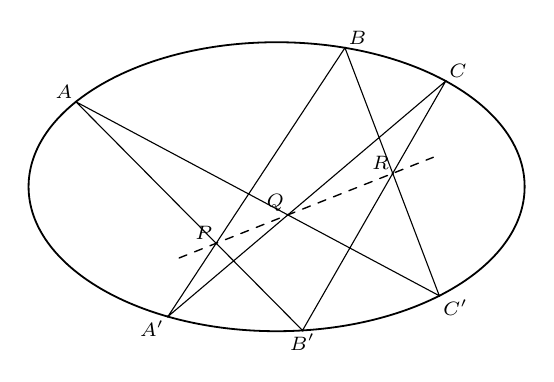
\begin{tikzpicture}[x=1mm,y=1mm,line cap=round,line join=round,
  every node/.style={font=\scriptsize,inner sep=1.15pt}]
  \draw[line width=.65pt] (0,0) ellipse (31.5 and 18.35);
  \coordinate (A) at (-25.484035,10.785859);
  \coordinate (B) at (8.682577,17.639152);
  \coordinate (C) at (21.482948,13.420340);
  \coordinate (Ap) at (-13.808691,-16.492871);
  \coordinate (Bp) at (3.292647,-18.249477);
  \coordinate (Cp) at (20.665859,-13.848921);
  \draw (A)--(Bp) (Ap)--(B) (A)--(Cp) (Ap)--(C) (B)--(Cp) (Bp)--(C);
  \draw[dashed,line width=.5pt] (-12.383512,-9.048797)--(19.907036,3.739890);
  \foreach \loc/\lab/\position in {A/A/above left,B/B/above right,C/C/above right,
    Ap/A'/below left,Bp/B'/below,Cp/C'/below right} {
    \fill (\loc) circle[radius=.44pt] node[\position] {$\lab$};
  }
  \foreach \x/\y/\lab in {-7.674474/-7.183780/P,1.426898/-3.579177/Q,14.749518/1.697252/R} {
    \fill (\x,\y) circle[radius=.44pt] node[above left] {$\lab$};
  }
\end{tikzpicture}}\par
\smallskip
\small\textbf{Figure 22.}\enspace Pascal's theorem.\par
}

\smallskip
\noindent\hypertarget{ex-V-4.6}{}\textbf{4.6.} Generalize (\Goto{result-V-4.5}{4.5}) as follows: given $13$ points $P_1,\dots,P_{13}$ in the plane, there are three additional determined points $P_{14},P_{15},P_{16}$, such that all quartic curves through $P_1,\dots,P_{13}$ also pass through $P_{14},P_{15},P_{16}$. What hypotheses are necessary on $P_1,\dots,P_{13}$ for this to be true?

\smallskip
\noindent\hypertarget{ex-V-4.7}{}\textbf{4.7.} If $D$ is any divisor of degree $d$ on the cubic surface (\Goto{result-V-4.7.3}{4.7.3}), show that
\[
p_a(D)\le
\begin{cases}
\tfrac16(d-1)(d-2)&\text{if }d\equiv1,2\pmod 3,\\[2pt]
\tfrac16(d-1)(d-2)+\tfrac23&\text{if }d\equiv0\pmod 3.
\end{cases}
\]
Show furthermore that for every $d>0$, this maximum is achieved by some irreducible nonsingular curve.

\smallskip
\noindent\hypertarget{ex-V-4.8}{}\textbf{*4.8.} Show that a divisor class $D$ on the cubic surface contains an irreducible curve $\Leftrightarrow$ it contains an irreducible nonsingular curve $\Leftrightarrow$ it is either (a) one of the $27$ lines, or (b) a conic (meaning a curve of degree $2$) with $D^2=0$, or (c) $D\cdot L\ge0$ for every}
% Contents from body/page-422.tex.
\ChapterSheet[10.6]{422}{408}{\Goto{p-370}{V\quad Surfaces}}{%
\noindent line $L$, and $D^2>0$. [\emph{Hint:} Generalize (\Goto{result-V-4.11}{4.11}) to the surfaces obtained by blowing up $2$, $3$, $4$, or $5$ points of $\mathbf P^2$, and combine with our earlier results about curves on $\mathbf P^1\times\mathbf P^1$ and the rational ruled surface $X_1$, (\Goto{result-V-2.18}{2.18}).]

\smallskip
\noindent\hypertarget{ex-V-4.9}{}\textbf{4.9.} If $C$ is an irreducible non-singular curve of degree $d$ on the cubic surface, and if the genus $g>0$, then
\[
g\ge
\begin{cases}
\tfrac12(d-6)&\text{if $d$ is even, $d\ge8$,}\\[2pt]
\tfrac12(d-5)&\text{if $d$ is odd, $d\ge13$,}
\end{cases}
\]
and this minimum value of $g>0$ is achieved for each $d$ in the range given.

\smallskip
\noindent\hypertarget{ex-V-4.10}{}\textbf{4.10.} A curious consequence of the implication (iv) $\Rightarrow$ (iii) of (\Goto{result-V-4.11}{4.11}) is the following numerical fact: Given integers $a,b_1,\dots,b_6$ such that $b_i>0$ for each $i$, $a-b_i-b_j>0$ \EditionText{for distinct $i,j$} and $2a-\sum_{i\ne j}b_i>0$ for each $j$, we must necessarily have $a^2-\sum b_i^2>0$. Prove this directly (for $a,b_1,\dots,b_6\in\mathbf R$) using methods of freshman calculus.

\smallskip
\noindent\hypertarget{ex-V-4.11}{}\textbf{4.11.} \emph{The Weyl Groups.} Given any diagram consisting of points and line segments joining some of them, we define an abstract group, given by generators and relations, as follows: each point represents a generator $x_i$. The relations are $x_i^2=1$ for each $i$; $(x_ix_j)^2=1$ if $i$ and $j$ are not joined by a line segment, and $(x_ix_j)^3=1$ if $i$ and $j$ are joined by a line segment.

\noindent\hangindent=2.5em\hspace*{1.25em}(a) The \emph{Weyl group} $\mathbf A_n$ is defined using the diagram
\[
\begin{tikzpicture}[x=.42cm,y=.42cm]
\draw (0,0)--(2,0) (4.4,0)--(5.25,0);
\foreach \x in {0,1,2,5.25} \draw[fill=white] (\x,0) circle[radius=1.6pt];
\node at (3.35,.07) {$\dots$};
\end{tikzpicture}
\]
\noindent\hangindent=2.5em\hspace*{2.5em}of $n-1$ points, each joined to the next. Show that it is isomorphic to the symmetric group $\Sigma_n$ as follows: map the generators of $\mathbf A_n$ to the elements $(12),(23),\dots,(n-1\,n)$ of $\Sigma_n$, to get a surjective homomorphism $\mathbf A_n\to\Sigma_n$. Then estimate the number of elements of $\mathbf A_n$ to show in fact it is an isomorphism.

\noindent\hangindent=2.5em\hspace*{1.25em}(b) The \emph{Weyl group} $\mathbf E_6$ is defined using the diagram
\[
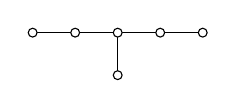
\begin{tikzpicture}[x=.54cm,y=.54cm]
\draw (0,0)--(4,0) (2,0)--(2,-1);
\foreach \x in {0,1,2,3,4} \draw[fill=white] (\x,0) circle[radius=1.6pt];
\draw[fill=white] (2,-1) circle[radius=1.6pt];
\end{tikzpicture}
\]
\noindent\hangindent=2.5em\hspace*{2.5em}Call the generators $x_1,\dots,x_5$ and $y$. Show that one obtains a surjective homomorphism $\mathbf E_6\to G$, the group of automorphisms of the configuration of $27$ lines (\Goto{result-V-4.10.1}{4.10.1}), by sending $x_1,\dots,x_5$ to the permutations $(12),(23),\dots,(56)$ of the $E_i$, respectively, and $y$ to the element associated with the quadratic transformation based at $P_1,P_2,P_3$.

\noindent\hangindent=2.5em\hspace*{.95em}*(c) Estimate the number of elements in $\mathbf E_6$, and thus conclude that $\mathbf E_6\cong G$.

\noindent\hangindent=1.3em\hspace*{1.3em}\emph{Note:} See Manin \Goto{bib-479-14}{[3, \S\S25, 26]} for more about Weyl groups, root systems, and exceptional curves.

\smallskip
\noindent\hypertarget{ex-V-4.12}{}\textbf{4.12.} Use (\Goto{result-V-4.11}{4.11}) to show that if $D$ is any ample divisor on the cubic surface $X$, then $H^1(X,\mathcal O_X(-D))=0$. This is Kodaira's vanishing theorem for the cubic surface (III, \Goto{result-III-7.15}{7.15}).

\smallskip
\noindent\hypertarget{ex-V-4.13}{}\textbf{4.13.} Let $X$ be the Del Pezzo surface of degree $4$ in $\mathbf P^4$ obtained by blowing up $5$ points of $\mathbf P^2$ (\Goto{result-V-4.7}{4.7}).

\noindent\hspace*{1.3em}(a) Show that $X$ contains $16$ lines.}
% Contents from body/page-423.tex.
\ChapterSheet[10.65]{423}{409}{\Goto{sec-V-5}{5\quad Birational Transformations}}{%
\noindent\hangindent=2.4em\hspace*{1.3em}(b) Show that $X$ is a complete intersection of two quadric hypersurfaces in $\mathbf P^4$ (the converse follows from (\Goto{result-V-4.7.1}{4.7.1})).

\smallskip
\noindent\hypertarget{ex-V-4.14}{}\textbf{4.14.} Using the method of (\Goto{result-V-4.13.1}{4.13.1}), verify that there are nonsingular curves in $\mathbf P^3$ with $d=8$, $g=6,7$; $d=9$, $g=7,8,9$; $d=10$, $g=8,9,10,11$. Combining with (IV, \S\Goto{sec-IV-6}{6}), this completes the determination of all possible $g$ for curves of degree $d\le10$ in $\mathbf P^3$.

\smallskip
\noindent\hypertarget{ex-V-4.15}{}\textbf{4.15.} Let $P_1,\dots,P_r$ be a finite set of (ordinary) points of $\mathbf P^2$, no $3$ collinear. We define an \emph{admissible transformation} to be a quadratic transformation (\Goto{result-V-4.2.3}{4.2.3}) centered at some three of the $P_i$ (call them $P_1,P_2,P_3$). This gives a new $\mathbf P^2$, and a new set of $r$ points, namely $Q_1,Q_2,Q_3$, and the images of $P_4,\dots,P_r$. We say that $P_1,\dots,P_r$ are \emph{in general position} if no three are collinear, and furthermore after any finite sequence of admissible transformations, the new set of $r$ points also has no three collinear.

\noindent\hangindent=2.5em\hspace*{1.2em}(a) A set of $6$ points is in general position if and only if no three are collinear and not all six lie on a conic.

\noindent\hangindent=2.5em\hspace*{1.2em}(b) If $P_1,\dots,P_r$ are in general position, then the $r$ points obtained by any finite sequence of admissible transformations are also in general position.

\noindent\hangindent=2.5em\hspace*{1.2em}(c) Assume the ground field $k$ is uncountable. Then given $P_1,\dots,P_r$ in general position, there is a dense subset $V\subseteq\mathbf P^2$ such that for any $P_{r+1}\in V$, $P_1,\dots,P_{r+1}$ will be in general position. [\emph{Hint:} Prove a lemma that when $k$ is uncountable, a variety cannot be equal to the union of a countable family of proper closed subsets.]

\noindent\hangindent=2.5em\hspace*{1.2em}(d) Now take $P_1,\dots,P_r\in\mathbf P^2$ in general position, and let $X$ be the surface obtained by blowing up $P_1,\dots,P_r$. If $r=7$, show that $X$ has exactly $56$ irreducible nonsingular curves $C$ with $g=0$, $C^2=-1$, and that these are the only irreducible curves with negative self-intersection. Ditto for $r=8$, the number being $240$.

\noindent\hangindent=2.5em\hspace*{.9em}*(e) For $r=9$, show that the surface $X$ defined in (d) has infinitely many irreducible nonsingular curves $C$ with $g=0$ and $C^2=-1$. [\emph{Hint:} Let $L$ be the line joining $P_1$ and $P_2$. Show that there exist finite sequences of admissible transformations such that the strict transform of $L$ becomes a plane curve of arbitrarily high degree.] This example is apparently due to Kodaira---see Nagata \Goto{bib-nagata-5}{[5, II, p.~283]}.

\smallskip
\noindent\hypertarget{ex-V-4.16}{}\textbf{4.16.} \EditionText{Assume $\operatorname{char}k\ne3$. }For the \emph{Fermat cubic surface} $x_0^3+x_1^3+x_2^3+x_3^3=0$, find the equations of the $27$ lines explicitly, and verify their incidence relations. What is the group of automorphisms of this surface?

\bigskip
\noindent\hypertarget{sec-V-5}{}\BookMark{1}{5.5  Birational Transformations}{sec-V-5}\textbf{\large 5\quad Birational Transformations}\par\medskip
\noindent Up to now we have dealt with one surface at a time, or a surface and its monoidal transforms. Now we will show that in fact any birational transformation of (nonsingular projective) surfaces can be factored into a finite sequence of monoidal transformations and their inverses. This confirms the central role played by the monoidal transformations in the study of surfaces. A consequence of this result is the fact that the arithmetic genus of a surface is a \emph{birational} invariant.}
% Contents from body/page-424.tex.
\ChapterSheet{424}{410}{\Goto{p-370}{V\quad Surfaces}}{%
In this section we will also prove Castelnuovo's criterion for contracting exceptional curves of the first kind, and deduce the existence of relatively minimal models for surfaces. See Shafarevich \Goto{bib-482-7}{[1, Ch.~I, II]}, Zariski \Goto{bib-zariski-5}{[5]}, and Zariski \Goto{bib-zariski-10}{[10, Ch.~IV]} as general references.

We begin by recalling some general facts about birational maps between varieties of any dimension, including Zariski's Main Theorem.

\medskip
Let $X$ and $Y$ be projective varieties of any dimension. Recall (I, \S\Goto{sec-I-4}{4}) that to give a birational transformation $T$ from $X$ to $Y$ is to give an open subset $U\subseteq X$ and a morphism $\varphi\colon U\to Y$ which induces an isomorphism of function fields $K(Y)\cong K(X)$. If we have another open set $V\subseteq X$ and another morphism $\psi\colon V\to Y$ representing $T$, then $\varphi$ and $\psi$ agree where both are defined, so we can glue them to obtain a morphism defined on $U\cup V$ (I, Ex.~\Goto{ex-I-4.2}{4.2}). So there is a largest open set $U\subseteq X$ on which $T$ is represented by a morphism $\varphi\colon U\to Y$. We say that $T$ is \emph{defined} at the points of $U$, and we call the points of $X-U$ \emph{fundamental points} of $T$.

Now let $T\colon X\to Y$ be a birational transformation, represented by the morphism $\varphi\colon U\to Y$. Let $\Gamma_0\subseteq U\times Y$ be the graph of $\varphi$, and let $\Gamma\subseteq X\times Y$ be the closure of $\Gamma_0$. We call $\Gamma$ the \emph{graph} of $T$. For any subset $Z\subseteq X$, we define $T(Z)$ to be $p_2(p_1^{-1}(Z))$, where $p_1$ and $p_2$ are the projections of $\Gamma$ to $X$ and $Y$. We call $T(Z)$ the \emph{total transform} of $Z$. If $T$ is defined at a point $P$, then $T(P)$ will be the point $\varphi(P)$. However, if $P$ is a fundamental point of $T$, then in general $T(P)$ will consist of more than one point.

\medskip
\noindent\hypertarget{result-V-5.1}{}\textbf{Lemma 5.1.} \emph{If $T\colon X\to Y$ is a birational transformation of projective varieties, and if $X$ is normal, then the fundamental points of $T$ form a closed subset of codimension $\ge2$.}

\smallskip
\noindent\textsc{Proof.} If $P\in X$ is a point of codimension $1$, then $\mathcal O_{P,X}$ is a discrete valuation ring. Since $T$ is defined at the generic point of $X$, and $Y$ is projective, hence proper, it follows from the valuative criterion of properness (II, \Goto{result-II-4.7}{4.7}) that $T$ is also defined at $P$. (We have already used this argument in the proof of (II, \Goto{result-II-8.19}{8.19}), to show that the geometric genus is a birational invariant.)

\medskip
\noindent\hypertarget{result-V-5.1.1}{}\textbf{Example 5.1.1.} Let $X$ be a surface, and let $\pi\colon\widetilde X\to X$ be the monoidal transformation with center $P$. Then $\pi$ is defined everywhere. Its inverse $\pi^{-1}\colon X\to\widetilde X$ is a birational transformation having $P$ as a fundamental point.

\medskip
\noindent\hypertarget{result-V-5.2}{}\textbf{Theorem 5.2} (Zariski's Main Theorem). \emph{Let $T\colon X\to Y$ be a birational transformation of projective varieties, and assume that $X$ is normal. If $P$ is a fundamental point of $T$, then the total transform $T(P)$ is connected and of dimension $\ge1$.}

\smallskip
\noindent\textsc{Proof.} This is just a variant of the earlier form of Zariski's Main Theorem (III, \Goto{result-III-11.4}{11.4}). Let $\Gamma$ be the graph of $T$, and consider the morphism $p_1\colon\Gamma\to X$. This is a birational projective morphism, so by (III, \Goto{result-III-11.4}{11.4}), $p_1^{-1}(P)$ is connected.}
% Contents from body/page-425.tex.
\ChapterSheet[10.65]{425}{411}{\Goto{sec-V-5}{5\quad Birational Transformations}}{%
\noindent If it has dimension $0$, then the same is true in a neighborhood $V$ of $P$ (II, Ex.~\Goto{ex-II-3.22}{3.22}). In that case $p_1^{-1}(V)\to V$ is a projective, birational morphism, with finite fibres, so it is a finite morphism (III, Ex.~\Goto{ex-III-11.2}{11.2}). But $V$ is normal, so it must be an isomorphism. This says that $T$ is defined at $P$, which is a contradiction. We conclude that $p_1^{-1}(P)$ is connected of dimension $\ge1$. Since $p_2$ maps this set isomorphically onto $T(P)$, we have the result.

\medskip
Now we come to the key result which enables us to factor birational transformations of surfaces.

\medskip
\noindent\hypertarget{result-V-5.3}{}\textbf{Proposition 5.3.} \emph{Let $f\colon X'\to X$ be a birational morphism of (nonsingular, projective) surfaces. Let $P$ be a fundamental point of $f^{-1}$. Then $f$ factors through the monoidal transformation $\pi\colon\widetilde X\to X$ with center $P$.}

\smallskip
\noindent\textsc{Proof.} Let $T$ be the birational transformation of $X'$ to $\widetilde X$ defined as $\pi^{-1}\circ f$. Our object is to show that $T$ is a morphism. If not, then it has a fundamental (closed) point $P'$. Clearly $f(P')=P$. Furthermore $T(P')$ has dimension $\ge1$ in $\widetilde X$, by (\Goto{result-V-5.2}{5.2}). Thus $T(P')$ must be the exceptional curve $E$ of $\pi$.

On the other hand, by (\Goto{result-V-5.1}{5.1}), $T^{-1}$ is defined at all except finitely many points of $\widetilde X$, so we can find a closed point $Q\in E$ where $T^{-1}$ is defined, and hence $T^{-1}(Q)=P'$. We will show that this situation leads to a contradiction.

Choose local coordinates $x,y$ at $P$ on $X$. Then as in the proof of (\Goto{result-V-3.6}{3.6}), there is an open neighborhood $V$ of $P$ such that $\pi^{-1}(V)$ is defined by the equation $ty-ux$ in $\mathbf P^1_V$. By a linear change of variables in $x,y$ and $t,u$, we may assume that $Q$ is the point $t=0$, $u=1$ in $E$. Then $t,y$ form local coordinates at $Q$ on $\widetilde X$; the local equation of $E$ is $y=0$, and $x=ty$.

Since $P$ is a fundamental point of $f^{-1}$, by (\Goto{result-V-5.2}{5.2}) we have $f^{-1}(P)$ connected of dimension $\ge1$, so there is an irreducible curve $C$ in $f^{-1}(P)$ containing $P'$. Let $z=0$ be a local equation for $C$ at $P'$.

Since $f^{-1}(P)$ is defined by $x=y=0$, the images of $x,y$ in $\mathcal O_{P'}$ are in the ideal generated by $z$, so we can write $x=az$, $y=bz$, $a,b\in\mathcal O_{P'}$. On the other hand, $\mathcal O_Q$ dominates $\mathcal O_{P'}$. (We consider $\mathcal O_P,\mathcal O_{P'},\mathcal O_Q$ all as subrings of the common function field $K$ of $X,X',\widetilde X$.) Since $t,y$ are local coordinates at $Q$, $y\notin\mathfrak m_Q^2$, so we conclude that $y\notin\mathfrak m_{P'}^2$ in $\mathcal O_{P'}$. Therefore $b$ is a unit in $\mathcal O_{P'}$, and so $t=x/y=a/b$ is in the local ring $\mathcal O_{P'}$. Since $t\in\mathfrak m_Q$, we must have $t\in\mathfrak m_{P'}$.

Now we use the fact that $T(P')=E$. This implies that for any $w\in\mathfrak m_{P'}$, the image of $w$ in $\mathcal O_Q$ must be contained in the ideal generated by $y$, since $y$ is the local equation for $E$. In particular, taking $w=t$, we find $t\in(y)$, which is a contradiction, since $t$ and $y$ are local coordinates at $Q$.

\medskip
\noindent\hypertarget{result-V-5.4}{}\textbf{Corollary 5.4.} \emph{Let $f\colon X'\to X$ be a birational morphism of surfaces. Let $n(f)$ be the number of irreducible curves $C'\subseteq X'$ such that $f(C')$ is a point. Then $n(f)$ is finite and $f$ can be factored into a composition of exactly $n(f)$ monoidal transformations.}}
% Contents from body/page-426.tex.
\ChapterSheet{426}{412}{\Goto{p-370}{V\quad Surfaces}}{%
\noindent\textsc{Proof.} If $f(C')$ is a point $P$, then $P$ is a fundamental point of $f^{-1}$. By (\Goto{result-V-5.1}{5.1}) the fundamental points of $f^{-1}$ form a finite set, and for each one, its inverse image $f^{-1}(P)$ is a closed subset of $X'$, having only finitely many irreducible components, so the set of curves $C'$ which are mapped to a point is finite.

Now let $P$ be a fundamental point of $f^{-1}$. Then by (\Goto{result-V-5.3}{5.3}) $f$ factors through the monoidal transformation $\pi\colon\widetilde X\to X$ with center $P$, i.e., $f=\pi\circ f_1$ for some morphism $f_1\colon X'\to\widetilde X$. We will show that $n(f_1)=n(f)-1$. Indeed, if $f_1(C')$ is a point, then certainly $f(C')$ is a point. Conversely, if $f(C')$ is a point, then either $f_1(C')$ is a point, or $f_1(C')=E$, the exceptional curve of $\pi$. Furthermore, since $f_1^{-1}$ is a morphism except at finitely many points, there is a unique irreducible curve $E'$ in $X'$ with $f_1(E')=E$. Thus $n(f_1)=n(f)-1$.

Continuing in this fashion, after factoring through $n(f)$ monoidal transformations, we reduce to a morphism with $n(f)=0$. But by (\Goto{result-V-5.2}{5.2}), \EditionText{its inverse birational map has no fundamental points}, so it is an isomorphism. Thus $f$ is factored into $n(f)$ monoidal transformations.

\medskip
\noindent\hypertarget{result-V-5.4.1}{}\textbf{Remark 5.4.1.} It is interesting to compare the factorization of (\Goto{result-V-5.3}{5.3}) with the universal property of blowing up proved in (II, \Goto{result-II-7.14}{7.14}). While the new result implies the old one in the special case of blowing up a point (since $f^{-1}\mathfrak m_P\cdot\mathcal O_{X'}$ being invertible implies $f^{-1}(P)$ has dimension $1$, so $P$ is a fundamental point), it is actually stronger, since it uses Zariski's Main Theorem. We cannot deduce (\Goto{result-V-5.3}{5.3}) from (II, \Goto{result-II-7.14}{7.14}), because the hypothesis that $f^{-1}\mathfrak m_P\cdot\mathcal O_{X'}$ is invertible is impossible to verify in our case.

\medskip
\noindent\hypertarget{result-V-5.4.2}{}\textbf{Remark 5.4.2.} Comparing (\Goto{result-V-5.4}{5.4}) to the earlier theorem (II, \Goto{result-II-7.17}{7.17}), we see that the new result is more precise, because it uses only monoidal transformations, rather than the more general concept of blowing up an arbitrary sheaf of ideals.

\medskip
\noindent\hypertarget{result-V-5.4.3}{}\textbf{Remark 5.4.3.} It is easy to see that (\Goto{result-V-5.3}{5.3}) is false for nonsingular projective varieties of dimension $\ge3$. For example, let $f\colon X'\to X$ be the blowing-up of a nonsingular curve $C$ in a nonsingular projective $3$-fold $X$. Then any point $P\in C$ is a fundamental point of $f^{-1}$, but $f$ cannot factor through the monoidal transformation $\pi\colon\widetilde X\to X$ with center $P$, because $f^{-1}(P)$ has dimension $1$, while $\pi^{-1}(P)$ has dimension $2$.

\medskip
\noindent\hypertarget{result-V-5.4.4}{}\textbf{Remark 5.4.4.} The example (\Goto{result-V-5.4.3}{5.4.3}) suggests posing the following modified problem: given a birational morphism $f\colon X'\to X$ of nonsingular projective varieties, is it possible to factor $f$ into a finite succession of monoidal transformations along nonsingular subvarieties? This is also false in dimension $\ge3$: see Sally \Goto{bib-sally-1}{[1]} and Shannon \Goto{bib-482-8-item-1}{[1]}.

\medskip
\noindent\hypertarget{result-V-5.5}{}\textbf{Theorem 5.5.} \emph{Let $T\colon X\to X'$ be a birational transformation of surfaces. Then it is possible to factor $T$ into a finite sequence of monoidal transformations and their inverses.}}
% Contents from body/page-427.tex.
\ChapterSheet[10.6]{427}{413}{\Goto{sec-V-5}{5\quad Birational Transformations}}{%
\noindent\textsc{Proof.} Using (\Goto{result-V-5.4}{5.4}), it will be sufficient to show that there is a surface $X''$, and birational morphisms $f\colon X''\to X$ and $g\colon X''\to X'$ such that $T=g\circ f^{-1}$. To construct $X''$, we proceed as follows.

Let $H'$ be a very ample divisor on $X'$, and let $C'$ be an irreducible nonsingular curve in the linear system $|2H'|$, which does not pass through any of the fundamental points of $T^{-1}$. In other words, $C'$ is entirely contained in the largest open set $U'\subseteq X'$ on which $T^{-1}$ is represented by a morphism $\varphi\colon U'\to X$. Let $C=\varphi(C')$ be the image of $C'$ in $X$. We define an integer $m$ by $m=p_a(C)-p_a(C')$. Since we have a finite birational morphism of $C'$ to $C$, we see that $m\ge0$, and $m=0$ if and only if $C'$ is isomorphic to $C$ (IV, Ex.~\Goto{ex-IV-1.8}{1.8}). Note also that if we replace $C'$ by a linearly equivalent curve $C'_1$, also missing the fundamental points of $T^{-1}$, then $C_1=\varphi(C'_1)$ is linearly equivalent to $C$. In fact, if $C'-C'_1=(f)$ for some rational function $f$ on $X'$, then $C-C_1=(f)$ on $X$. Since the arithmetic genus of a curve depends only on its linear equivalence class (Ex.~\Goto{ex-V-1.3}{1.3}), we see that the integer $m$ depends only on $T$ and $H'$, and not on the particular curve $C'\in|2H'|$ chosen.

Now fix $C'$ temporarily. If $m>0$, then $C$ must be singular. Let $P$ be a singular point of $C$, let $\pi\colon\widetilde X\to X$ be the monoidal transformation with center $P$, and let $\widetilde C$ be the strict transform of $C$. Then by (\Goto{result-V-3.7}{3.7}), $p_a(\widetilde C)<p_a(C)$. Thus if $\widetilde T=T\circ\pi$, then $m(\widetilde T)<m(T)$.

Continuing in this fashion, as in the proof of (\Goto{result-V-3.8}{3.8}), we see that there is a morphism $f\colon X''\to X$, obtained by a finite number of monoidal transformations, such that if $T'=T\circ f$, then $m(T')=0$.

We will show that in fact $T'$ is a morphism. If not, then $T'$ will have a fundamental point $P$. By (\Goto{result-V-5.2}{5.2}), $T'(P)$ contains an irreducible curve $E'\subseteq X'$. Since $H'$ is very ample, $E'\cdot H'>0$, and so $C'\cdot E'\ge2$ for any $C'\in|2H'|$. Let us choose $C'$, not containing any fundamental point of $T'^{-1}$, such that $C'$ meets $E'$ transversally (\Goto{result-V-1.2}{1.2}). Then $C'$ meets $E'$ in at least two distinct points, so the corresponding curve $C$ in $X''$ has at least a double point at $P$. But this contradicts $m(T')=0$.

We conclude that $T'$ is a morphism of $X''$ to $X'$, so that applying (\Goto{result-V-5.4}{5.4}) completes the proof, as mentioned above.

\medskip
\noindent\hypertarget{result-V-5.6}{}\textbf{Corollary 5.6.} \emph{The arithmetic genus of a nonsingular projective surface is a birational invariant.}

\smallskip
\noindent\textsc{Proof.} Indeed, $p_a$ is unchanged by a monoidal transformation (\Goto{result-V-3.5}{3.5}), so this follows directly from the theorem.

\medskip
\noindent\hypertarget{result-V-5.6.1}{}\textbf{Remark 5.6.1.} Even though the factorization theorem (\Goto{result-V-5.5}{5.5}) in a form analogous to (\Goto{result-V-5.4.4}{5.4.4}) is false in dimension $\ge3$, Hironaka \Goto{bib-477-15}{[3]} is able to deduce the birational invariance of $p_a$, for nonsingular projective varieties over a field of characteristic $0$, from the following statement, which is a consequence of his resolution of singularities: If $T\colon X\to X'$ is any birational transformation of nonsingular projective varieties over a field of characteristic $0$, then there is a morphism $f\colon X''\to X$, obtained by a finite succession of monoidal}
% Contents from body/page-428.tex.
\ChapterSheet[10.6]{428}{414}{\Goto{p-370}{V\quad Surfaces}}{%
\noindent transformations along nonsingular subvarieties, such that the birational map $T'=T\circ f$ is a morphism. There is another proof of the birational invariance of $p_a$, for varieties over $\mathbf C$, by Kodaira and Spencer \Goto{bib-478-17-item-1}{[1]}, using the equalities $h^{0q}=h^{q0}$ from Hodge theory, and the birational invariance of $h^{q0}$ (II, Ex.~\Goto{ex-II-8.8}{8.8}).

\medskip
Now we come to Castelnuovo's criterion for contracting a curve on a surface. We have seen that if $E$ is the exceptional curve of a monoidal transformation, then $E\cong\mathbf P^1$, and $E^2=-1$ (\Goto{result-V-3.1}{3.1}). In general, any curve $Y$ on a surface $X$, with $Y\cong\mathbf P^1$ and $Y^2=-1$ is classically called an \emph{exceptional curve of the first kind}. The following theorem tells us that any exceptional curve of the first kind is the exceptional curve of some monoidal transformation.

\medskip
\noindent\hypertarget{result-V-5.7}{}\textbf{Theorem 5.7} (Castelnuovo). \emph{If $Y$ is a curve on a surface $X$, with $Y\cong\mathbf P^1$ and $Y^2=-1$, then there exists a morphism $f\colon X\to X_0$ to a (nonsingular projective) surface $X_0$, and a point $P\in X_0$, such that $X$ is isomorphic via $f$ to the monoidal transformation of $X_0$ with center $P$, and $Y$ is the exceptional curve.}

\medskip
\noindent\textsc{Proof.} We will construct $X_0$ using the image of $X$ under a suitable morphism to a projective space. Choose a very ample divisor $H$ on $X$ such that $H^1(X,\mathcal L(H))=0$: for example, a sufficiently high multiple of any given very ample divisor (III, \Goto{result-III-5.2}{5.2}). Let $k=H\cdot Y$, and let us assume $k\ge2$. Then we will use the invertible sheaf $\mathcal M=\mathcal L(H+kY)$ to define a morphism of $X$ to $\mathbf P^N$.

\emph{Step 1.} First we prove that $H^1(X,\mathcal L(H+(k-1)Y))=0$. In fact, we will prove more generally that for every $i=0,1,\dots,k$, we have $H^1(X,\mathcal L(H+iY))=0$. For $i=0$, this is true by hypothesis, so we proceed by induction on $i$. Suppose it is true for $i-1$. We consider the exact sequence of sheaves
\[
0\to\mathcal L(H+(i-1)Y)\to\mathcal L(H+iY)\to\mathcal O_Y\otimes\mathcal L(H+iY)\to0.
\]
Now $Y\cong\mathbf P^1$, and $(H+iY)\cdot Y=k-i$, so
\[
\mathcal O_Y\otimes\mathcal L(H+iY)\cong\mathcal O_{\mathbf P^1}(k-i).
\]
We get an exact cohomology sequence
\[
\begin{aligned}
\dots&\to H^1(X,\mathcal L(H+(i-1)Y))\to H^1(X,\mathcal L(H+iY))\to{}\\
&\to H^1(\mathbf P^1,\mathcal O_{\mathbf P^1}(k-i))\to\dots.
\end{aligned}
\]
So from the induction hypothesis, and the known cohomology of $\mathbf P^1$, we conclude that $H^1(X,\mathcal L(H+iY))=0$ for any $i\le k$.

\emph{Step 2.} Next we show that $\mathcal M$ is generated by global sections. Since $H$ is very ample, the corresponding linear system $|H+kY|$ has no base points away from $Y$, so $\mathcal M$ is generated by global sections off $Y$. On the other hand,}
% Contents from body/page-429.tex.
\ChapterSheet[10.6]{429}{415}{\Goto{sec-V-5}{5\quad Birational Transformations}}{%
\setlength{\abovedisplayskip}{3.2pt}\setlength{\belowdisplayskip}{3.2pt}%
\noindent the natural map
\[
H^0(X,\mathcal M)\to H^0(Y,\mathcal M\otimes\mathcal O_Y)
\]
is surjective, because $\mathcal M\otimes\mathcal I_Y\cong\mathcal L(H+(k-1)Y)$, and
\[
H^1(X,\mathcal L(H+(k-1)Y))=0
\]
by Step 1. Next observe that $(H+kY)\cdot Y=0$, so $\mathcal M\otimes\mathcal O_Y\cong\mathcal O_{\mathbf P^1}$, which is generated by the global section $1$. Lifting this section to $H^0(X,\mathcal M)$, and using Nakayama's lemma, we see that $\mathcal M$ is generated by global sections also at every point of $Y$.

\emph{Step 3.} Therefore $\mathcal M$ determines a morphism $f_1\colon X\to\mathbf P^N$ (II, \Goto{result-II-7.1}{7.1}). Let $X_1$ be its image. Since $f_1^*\mathcal O(1)\cong\mathcal M$, and since the degree of $\mathcal M\otimes\mathcal O_Y$ is $0$, $f_1$ must map $Y$ to a point $P_1$. On the other hand, since $H$ is very ample, the linear system $|H+kY|$ separates points and tangent vectors away from $Y$, and also separates points of $Y$ from points not on $Y$, so $f_1$ is an isomorphism of $X-Y$ onto $X_1-P_1$ (II, \Goto{result-II-7.8.2}{7.8.2}).

\emph{Step 4.} Let $X_0$ be the normalization of $X_1$ (II, Ex.~\Goto{ex-II-3.8}{3.8}). Since $X$ is nonsingular, hence normal, the map $f_1$ factors to give a morphism $f\colon X\to X_0$. Since $Y$ is irreducible, $f(Y)$ is a point $P$, and since $X_1-P_1$ was nonsingular, we still have $f\colon X-Y\to X_0-P$ an isomorphism.

\emph{Step 5.} Now we will show that $X_0$ is nonsingular at the point $P$. Since in any case $X_0$ is normal, and $f$ is birational, we have $f_*\mathcal O_X\cong\mathcal O_{X_0}$ (see proof of (III, \Goto{result-III-11.4}{11.4})). So we can apply the theorem on formal functions (III, \Goto{result-III-11.1}{11.1}) to conclude that
\[
\widehat{\mathcal O}_P\cong\varprojlim H^0(Y_n,\mathcal O_{Y_n}),
\]
where $Y_n$ is the closed subscheme of $X$ defined by $\mathfrak m_P^n\cdot\mathcal O_X$. But since $f^{-1}(P)=Y$, the sequence of ideals $\mathfrak m_P^n\mathcal O_X$ is cofinal with the sequence of ideals $\mathcal I_Y^n$, so we may use these instead in the definition of $Y_n$ (II, \Goto{result-II-9.3.1}{9.3.1}).

We will show for each $n$ that $H^0(Y_n,\mathcal O_{Y_n})$ is isomorphic to a truncated power series ring $A_n=k[\![x,y]\!]/(x,y)^n$. It will follow that $\widehat{\mathcal O}_P\cong\varprojlim A_n\cong k[\![x,y]\!]$, which is a regular local ring. This in turn implies that $\mathcal O_P$ is regular (I, \Goto{result-I-5.4A}{5.4A}), hence $P$ is a nonsingular point.

For $n=1$, we have $H^0(Y,\mathcal O_Y)=k$. For $n>1$, we use the exact sequences
\[
0\to\mathcal I^n/\mathcal I^{n+1}\to\mathcal O_{Y_{n+1}}\to\mathcal O_{Y_n}\to0.
\]
Since $Y\cong\mathbf P^1$, and $Y^2=-1$, we have $\mathcal I/\mathcal I^2\cong\mathcal O_{\mathbf P^1}(1)$ by (\Goto{result-V-1.4.1}{1.4.1}), and $\mathcal I^n/\mathcal I^{n+1}\cong\mathcal O_{\mathbf P^1}(n)$ for each $n$, as in the proof of (\Goto{result-V-3.4}{3.4}). Taking cohomology, we have
\[
0\to H^0(\mathcal O_{\mathbf P^1}(n))\to H^0(\mathcal O_{Y_{n+1}})\to H^0(\mathcal O_{Y_n})\to0.
\]
For $n=1$, $H^0(\mathcal O_{\mathbf P^1}(1))$ is a $2$-dimensional vector space. Take a basis $x,y$. Then $H^0(\mathcal O_{Y_2})$, which in any case contains $k$, is seen to be isomorphic to $A_2$.

Now inductively, if $H^0(\mathcal O_{Y_n})$ is isomorphic to $A_n$, lift the elements $x,y$ to $H^0(\mathcal O_{Y_{n+1}})$. Since $H^0(\mathcal O_{\mathbf P^1}(n))$ is the vector space with basis $x^n,x^{n-1}y,\dots,y^n$, we see that $H^0(\mathcal O_{Y_{n+1}})\cong A_{n+1}$. Now as above we see that $P$ is a nonsingular point.}
% Contents from body/page-430.tex.
\ChapterSheet[10.55]{430}{416}{\Goto{p-370}{V\quad Surfaces}}{%
\emph{Step 6.} We complete the proof using the factorization theorem (\Goto{result-V-5.4}{5.4}). Since $X_0$ is nonsingular, we can apply (\Goto{result-V-5.4}{5.4}) to $f\colon X\to X_0$. We have $n(f)=1$ by construction, so $f$ must be the monoidal transformation with center $P$.

\emph{Step 7.} As an addendum, we show in fact that $X_0=X_1$, so the normalization was unnecessary. The natural map
\[
H^0(X,\mathcal M\otimes\mathcal I_Y)\to H^0(Y,\mathcal M\otimes\mathcal I_Y/\mathcal I_Y^2)
\]
is surjective, because the next term of the cohomology sequence is $H^1(X,\mathcal L(H+(k-2)Y))$, which is $0$ by Step 1. Since $\mathcal M\otimes\mathcal O_Y\cong\mathcal O_Y$, this shows that there are global sections $s,t\in H^0(X,\mathcal M\otimes\mathcal I_Y)\subseteq H^0(X,\mathcal M)$, which map to the parameters $x,y\in H^0(\mathcal O_{Y_2})\cong A_2$. On the other hand, these sections $s,t$ become sections of $\mathcal O(1)$ on $\mathbf P^N$, defining hyperplanes containing $P_1$. So they give elements $\bar s,\bar t\in\mathfrak m_{P_1}$, whose images in $\mathcal O_P$ generate the maximal ideal $\mathfrak m_P$. Since in any case $\mathcal O_P$ is a finitely generated $\mathcal O_{P_1}$-module, we conclude that $\mathcal O_P\cong\mathcal O_{P_1}$ (II, \Goto{result-II-7.4}{7.4}), and so $X_0\cong X_1$.

\medskip
\noindent\hypertarget{result-V-5.7.1}{}\textbf{Example 5.7.1.} Let $\pi\colon X\to C$ be a geometrically ruled surface (\S\Goto{sec-V-2}{2}), let $P$ be a point of $X$, and let $L$ be the fibre of $\pi$ containing $P$. Let $f\colon\widetilde X\to X$ be the monoidal transformation with center $P$. Then the strict transform $\widetilde L$ of $L$ on $\widetilde X$ is isomorphic to $\mathbf P^1$, and has $\widetilde L^2=-1$. Indeed, $L^2=0$ by (\Goto{result-V-2.3}{2.3}), and $P$ is a nonsingular point of $L$, so $\widetilde L\sim f^*L-E$ by (\Goto{result-V-3.6}{3.6}). It follows that $\widetilde L^2=-1$. Therefore by the theorem, we can blow down $\widetilde L$. In other words, there is a morphism $g\colon\widetilde X\to X'$ sending $\widetilde L$ to a point $Q$, and such that $g$ is the monoidal transformation with center $Q$. If $M=g(E)$, then $M\cong\mathbf P^1$ and $M^2=0$, for a similar reason to the above. Note also that the rational map $\pi'\colon X'\to C$ obtained from $\pi$ on $X-L\cong X'-M$ is in fact a morphism. Therefore $\pi'\colon X'\to C$ is another geometrically ruled surface. Indeed, the fibres of $\pi'$ are all isomorphic to $\mathbf P^1$, and since $\pi$ has a section, its strict transform on $X'$ will be a section of $\pi'$. This new ruled surface is called the \emph{elementary transform of $X$ with center $P$}, and is denoted by $\operatorname{elm}_P X$ (Fig.~\Goto{fig-book-23}{23}). See (Ex.~\Goto{ex-V-5.5}{5.5}) for some applications.

{\centering
\hypertarget{fig-book-23}{}%
\resizebox{.81\linewidth}{!}{%
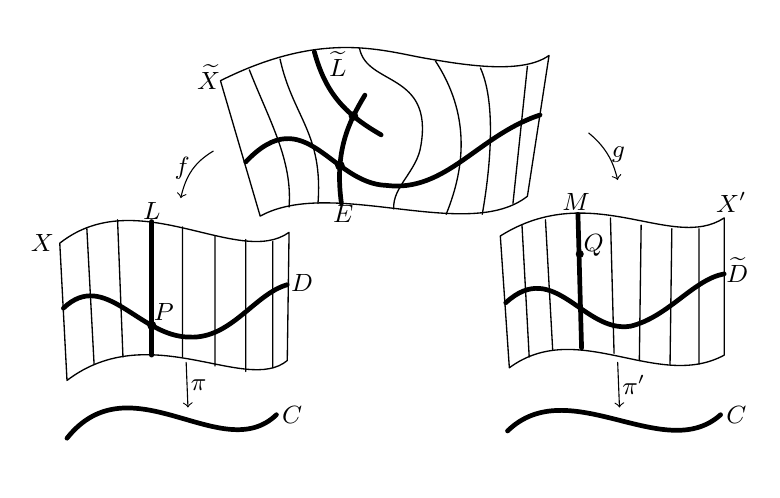
\begin{tikzpicture}[x=.65bp,y=-.65bp,line cap=round,line join=round,
 every node/.style={font=\small,inner sep=1.2pt},
 sheet/.style={line width=.48pt}, curve/.style={line width=1.7pt}]
% The blown-up middle sheet, including the bend in its ruling.
\draw[sheet] (103,20) .. controls (161,-9) and (194,4) .. (219,8)
  .. controls (242,12) and (271,16) .. (285,6)
  --(273,84) .. controls (240,110) and (165,73) .. (125,95) -- cycle;
\draw[sheet] (119,14) .. controls (130,42) and (143,64) .. (141,90);
\draw[sheet] (136,8) .. controls (143,40) and (160,49) .. (157,88);
\draw[sheet] (180,2) .. controls (184,23) and (221,15) .. (214,56)
  .. controls (212,70) and (198,79) .. (199,91);
\draw[sheet] (222,9) .. controls (241,38) and (239,67) .. (228,94);
\draw[sheet] (247,13) .. controls (257,35) and (251,77) .. (248,94);
\draw[sheet] (273,12) -- (265,88);
\draw[curve] (117,65) .. controls (150,30) and (164,77) .. (195,78)
  .. controls (228,82) and (246,50) .. (280,39);
\draw[curve] (155,4) .. controls (161,26) and (171,38) .. (192,50);
\draw[curve] (170,88) .. controls (166,59) and (174,43) .. (183,28);
\fill (176.64,39.57) circle[radius=1.75pt] (169.17,67.02) circle[radius=1.75pt];
\node[left] at (105,18) {$\widetilde X$};
\node[right] at (161,11) {$\widetilde L$};
\node[below] at (171,87) {$E$};
% Original ruled surface and its fibre over the marked point.
\draw[sheet] (14,110) .. controls (57,76) and (113,124) .. (141,104)
  --(140,175) .. controls (117,194) and (64,151) .. (18,186) -- cycle;
\draw[sheet] (29,102)--(33,177) (46,97)--(49,173) (82,101)--(82,173)
  (100,106)--(100,178) (117,108)--(117,181) (132,109)--(132,179);
\draw[curve] (16,146) .. controls (39,124) and (58,162) .. (86,162)
  .. controls (109,163) and (122,138) .. (140,133);
\draw[curve] (65,98)--(65,172);
\fill (65,155.60) circle[radius=1.65pt];
\node[left] at (13,110) {$X$};
\node[above] at (65,99) {$L$};
\node[right] at (64,148) {$P$};
\node[right] at (140,132) {$D$};
% The transformed ruled surface and its new fibre.
\draw[sheet] (258,106) .. controls (309,74) and (353,115) .. (382,96)
  --(382,172) .. controls (345,192) and (301,151) .. (263,179) -- cycle;
\draw[sheet] (270,100)--(274,173) (283,97)--(287,169) (319,96)--(321,171)
  (336,100)--(335,175) (353,102)--(352,177) (368,102)--(368,177);
\draw[curve] (261,143) .. controls (288,118) and (304,160) .. (330,156)
  .. controls (351,151) and (365,130) .. (382,127);
\draw[curve] (301,94)--(303,168);
\fill (302,116) circle[radius=1.45pt];
\node[above] at (300,94) {$M$};
\node[right] at (302,111) {$Q$};
\node[above] at (386,95) {$X'$};
\node[right] at (381,125) {$\widetilde D$};
\draw[->] (99,59) .. controls (89,65) and (84,72) .. (81,85) node[pos=.46,left] {$f$};
\draw[->] (307,49) .. controls (318,58) and (321,67) .. (323,75) node[pos=.45,right] {$g$};
\draw[->] (84,176)--(85,201) node[midway,right] {$\pi$};
\draw[->] (323,176)--(324,201) node[midway,right] {$\pi'$};
\draw[curve] (18,218) .. controls (53,174) and (104,234) .. (134,205) node[right] {$C$};
\draw[curve] (262,214) .. controls (296,181) and (349,233) .. (380,205) node[right] {$C$};
\end{tikzpicture}}\par
\smallskip
\small\textbf{Figure 23.}\enspace An elementary transformation of a ruled surface.\par
}}
% Contents from body/page-431.tex.
\ChapterSheet[10.55]{431}{417}{\Goto{sec-V-5}{5\quad Birational Transformations}}{%
\noindent\hypertarget{result-V-5.7.2}{}\textbf{Remark 5.7.2} (The General Contraction Problem). With the theorem of Castelnuovo (\Goto{result-V-5.7}{5.7}) in mind, one can pose the following general problem: Given a variety $X$, and a closed subset $Y\subseteq X$, find necessary and sufficient conditions for the existence of a birational morphism $f\colon X\to X_0$ such that $f(Y)$ is a single point $P$, and $f\colon X-Y\to X_0-P$ is an isomorphism. If such a morphism exists, we say that $Y$ is \emph{contractible}. A number of special cases of this problem have been treated, but a general solution is unknown. See Artin \Goto{bib-473-3}{[3]}, \Goto{bib-473-4}{[4]}, Grauert \Goto{bib-grauert-2}{[2]}, and Mumford \Goto{bib-mumford-6}{[6]}.

In case $Y$ is an irreducible curve on a surface $X$, here is what is known. If we require $X_0$ to be nonsingular, then by (\Goto{result-V-5.7}{5.7}) the necessary and sufficient conditions are that $Y\cong\mathbf P^1$ and $Y^2=-1$. If we allow $X_0$ to be singular, then a necessary condition is that $Y^2<0$ (Ex.~\Goto{ex-V-5.7}{5.7}). If $Y\cong\mathbf P^1$, this condition is also sufficient (Ex.~\Goto{ex-V-5.2}{5.2}). If $Y$ is arbitrary, with $Y^2<0$, and if the base field is $\mathbf C$, then a theorem of Grauert \Goto{bib-grauert-2}{[2]} shows that $X_0$ exists as a complex analytic space. However, $Y$ may not be contractible to an algebraic variety, as we show in the following example.

\medskip
\noindent\hypertarget{result-V-5.7.3}{}\textbf{Example 5.7.3} (Hironaka). Let $Y_0$ be a nonsingular cubic curve in $\mathbf P^2$ over an uncountable algebraically closed field $k$ (e.g., $k=\mathbf C$). Fix an inflection point $P_0\in Y_0$ to be the origin of the group law on $Y_0$. Since the abelian group $Y_0$ is uncountable, and since the torsion points are countable (IV, \Goto{result-IV-4.8.1}{4.8.1}), the torsion-free part must have infinite rank. Therefore we can choose $10$ points $P_1,\dots,P_{10}\in Y_0$ which are linearly independent over $\mathbb Z$ in the group law.

Now blow up $P_1,\dots,P_{10}$ in $\mathbf P^2$, let $X$ be the resulting surface, and let $Y$ be the strict transform of $Y_0$. Since $Y_0^2=9$, and we have blown up $10$ points on $Y$, we have $Y^2=-1$, using (\Goto{result-V-3.6}{3.6}). So by Grauert's theorem (\Goto{result-V-5.7.2}{5.7.2}), if $k=\mathbf C$, then $Y$ in $X$ would be contractible to a complex analytic space. We will show, however, that $Y$ is not contractible to a point $P$ in an algebraic variety $X_0$. If it were, let $P\in U\subseteq X_0$ be an open affine neighborhood of $P$. Let $C'_0\subseteq U$ be a curve not containing $P$\EditionText{ whose inverse image is not exceptional for the original blow-up of $\mathbf P^2$. Such a curve can be chosen as a component of a general affine hyperplane section of $U$ avoiding $P$ and containing none of the relevant exceptional images}. Let $C_0\subseteq X_0$ be its closure, which still does not contain $P$. Then its inverse image in $X$ will be a curve $C\subseteq X$ which does not meet $Y$. The image of $C$ in $\mathbf P^2$ will be a curve $C^*$ which does not meet $Y_0$ except at the points $P_1,\dots,P_{10}$.

But this is impossible. Let $d=\deg C^*$. Then by B\'ezout's theorem (\Goto{result-V-1.4.2}{1.4.2}), $C^*\cdot Y_0=3d>0$. So we can write
\[
C^*\cdot Y_0=\sum_{i=1}^{10}n_iP_i
\]
on $Y_0$, with $n_i\ge0$, $\sum n_i=3d$. But $C^*\sim dL$, where $L$ is a line in $\mathbf P^2$, and $L\cdot Y_0\sim3P_0$, so we have
\[
\sum_{i=1}^{10}n_iP_i=0
\]
in the group law on $Y_0$ (IV, \Goto{result-IV-1.3.7}{1.3.7}). This contradicts the fact that $P_1,\dots,P_{10}$ were chosen to be linearly independent over $\mathbb Z$.}
% Contents from body/page-432.tex.
\ChapterSheet{432}{418}{\Goto{p-370}{V\quad Surfaces}}{%
To conclude this section, we will prove the existence of relatively minimal models of surfaces. The idea is to find, within each birational equivalence class of surfaces, one which is as canonical as possible. Since one can always blow up a point, there is never a unique nonsingular projective model of a function field, as in the case of curves. However, we can look for one which is minimal for the relation of domination. So we say that a (nonsingular projective) surface $X$ is a \emph{relatively minimal model} of its function field, if every birational morphism $f\colon X\to X'$ to another (nonsingular projective) surface $X'$ is necessarily an isomorphism. If $X$ is the unique relatively minimal model in its birational equivalence class, then we say that $X$ is a \emph{minimal model}. (This somewhat irregular use of the word \textquotedblleft{}minimal\textquotedblright{} is retained for historical reasons.)

\medskip
\noindent\hypertarget{result-V-5.8}{}\textbf{Theorem 5.8.} \emph{Every surface admits a birational morphism to a relatively minimal model.}

\smallskip
\noindent\textsc{Proof.} Combining (\Goto{result-V-5.4}{5.4}) and (\Goto{result-V-5.7}{5.7}), it is clear that a surface is a relatively minimal model if and only if it contains no exceptional curves of the first kind. So given a surface $X$, if it is already a relatively minimal model, stop. If not, let $Y$ be an exceptional curve of the first kind. By (\Goto{result-V-5.7}{5.7}) there is a morphism $X\to X_1$ contracting $Y$.

We continue in this manner, contracting exceptional curves of the first kind whenever one exists, and so we obtain a sequence of birational morphisms $X\to X_1\to X_2\to\dots$. We must show that this process eventually stops.

The following proof is due to Matsumura \Goto{bib-479-16-item-1}{[1]}. Suppose that we have a sequence of $n$ contractions
\[
X=X_0\to X_1\dots\to X_n
\]
as above. For each $i=1,\dots,n$, let $E'_i\subseteq X_{i-1}$ be the exceptional curve of the contraction $X_{i-1}\to X_i$, and let $E_i$ be its total transform on $X$. Then by (\Goto{result-V-3.2}{3.2}) we have $E_i^2=-1$ for each $i$, and $E_i\cdot E_j=0$ for $i\ne j$.

Now for each $i$, let $e_i=c(E_i)$ be the cohomology class of $E_i$ in $H^1(X,\Omega)$ (Ex.~\Goto{ex-V-1.8}{1.8}). Then we have $\langle e_i,e_i\rangle=-1$ and $\langle e_i,e_j\rangle=0$ in the intersection pairing on $H^1(X,\Omega)$, by (Ex.~\Goto{ex-V-1.8}{1.8}). It follows that $e_1,\dots,e_n$ are linearly independent elements of the vector space $H^1(X,\Omega)$ over $k$.

We conclude that $n\le\dim_kH^1(X,\Omega)$. Since this is a finite-dimensional vector space, $n$ is bounded, so the contraction process must terminate.

\emph{Note:} One can give another proof of this result by showing that the rank of the N\'eron--Severi group drops by $1$ with each contraction, so that $n\le\operatorname{rank}\operatorname{NS}(X)$, which is finite---Cf.\ (Ex.~\Goto{ex-V-1.7}{1.7}).

\medskip
\noindent\hypertarget{result-V-5.8.1}{}\textbf{Remark 5.8.1.} In spite of this result, it is \emph{not} true that a surface necessarily has only finitely many exceptional curves of the first kind. For example, if we blow up $r$ points in general position in $\mathbf P^2$, with $r\ge9$, then the resulting surface has infinitely many exceptional curves of the first kind (Ex.~\Goto{ex-V-4.15}{4.15}).}
% Contents from body/page-433.tex.
\ChapterSheet[10.55]{433}{419}{\Goto{sec-V-5}{5\quad Birational Transformations}}{%
\noindent\hypertarget{result-V-5.8.2}{}\textbf{Example 5.8.2.} In the birational equivalence class of rational surfaces, $\mathbf P^2$ is a relatively minimal model, and so is the rational ruled surface $X_e$ for each $e\ge0$, $e\ne1$. This follows easily from the determination of all irreducible curves on $X_e$ (\Goto{result-V-2.18}{2.18}). On the contrary, $X_1$ is not relatively minimal (\Goto{result-V-2.11.5}{2.11.5}).

\medskip
\noindent\hypertarget{result-V-5.8.3}{}\textbf{Example 5.8.3.} In the class of surfaces birational to $\mathbf P^1\times C$, where $C$ is a curve of genus $g>0$, every geometrically ruled surface $\pi\colon X\to C$ is relatively minimal. Indeed, if $Y$ is any rational curve in $X$, then $\pi(Y)$ is a point because of (IV, \Goto{result-IV-2.5.4}{2.5.4}). Thus $Y$ is a fibre of $\pi$, $Y^2=0$, and so we see that $X$ has no exceptional curves of the first kind.

\medskip
\noindent\hypertarget{result-V-5.8.4}{}\textbf{Remark 5.8.4.} A classical theorem, proved in all characteristics by Zariski \Goto{bib-zariski-5}{[5]}, \Goto{bib-zariski-6}{[6]}, \Goto{bib-483-20}{[9]} states that except for the rational and ruled surfaces, every surface is birational to a (unique) minimal model. One can also show that in the case of rational and ruled surfaces, every relatively minimal model is one of those listed in (\Goto{result-V-5.8.2}{5.8.2}) and (\Goto{result-V-5.8.3}{5.8.3}). See Nagata \Goto{bib-nagata-5}{[5]} or Hartshorne \Goto{bib-477-5}{[4]}.

\medskip
\noindent\textsc{Exercises}

\smallskip
\noindent\hypertarget{ex-V-5.1}{}\textbf{5.1.} Let $f$ be a rational function on the surface $X$. Show that it is possible to \textquotedblleft{}resolve the singularities of $f$\textquotedblright{} in the following sense: there is a birational morphism $g\colon X'\to X$ so that $f$ induces a morphism of $X'$ to $\mathbf P^1$. [\emph{Hints:} Write the divisor of $f$ as $(f)=\sum n_iC_i$. Then apply embedded resolution (\Goto{result-V-3.9}{3.9}) to the curve $Y=\bigcup C_i$. Then blow up further as necessary whenever a curve of zeros meets a curve of poles until the zeros and poles of $f$ are disjoint.]

\smallskip
\noindent\hypertarget{ex-V-5.2}{}\textbf{5.2.} Let $Y\cong\mathbf P^1$ be a curve in a surface $X$, with $Y^2<0$. Show that $Y$ is contractible (\Goto{result-V-5.7.2}{5.7.2}) to a point on a projective variety $X_0$ (in general singular).

\smallskip
\noindent\hypertarget{ex-V-5.3}{}\textbf{5.3.} If $\pi\colon\widetilde X\to X$ is a monoidal transformation with center $P$, show that $H^1(\widetilde X,\Omega_{\widetilde X})\cong H^1(X,\Omega_X)\oplus k$. This gives another proof of (\Goto{result-V-5.8}{5.8}). [\emph{Hints:} Use the projection formula (III, Ex.~\Goto{ex-III-8.3}{8.3}) and (III, Ex.~\Goto{ex-III-8.1}{8.1}) to show that $H^i(X,\Omega_X)\cong H^i(\widetilde X,\pi^*\Omega_X)$ for each $i$. Next use the exact sequence
\[
0\to\pi^*\Omega_X\to\Omega_{\widetilde X}\to\Omega_{\widetilde X/X}\to0
\]
and a local calculation with coordinates to show that there is a natural isomorphism $\Omega_{\widetilde X/X}\cong\Omega_E$, where $E$ is the exceptional curve. Now use the cohomology sequence of the above sequence (you will need every term) and Serre duality to get the result.]

\smallskip
\noindent\hypertarget{ex-V-5.4}{}\textbf{5.4.} Let $f\colon X\to X'$ be a birational morphism of nonsingular surfaces.

\noindent\hangindent=2.4em\hspace*{1.15em}(a) If $Y\subseteq X$ is an irreducible curve such that $f(Y)$ is a point, then $Y\cong\mathbf P^1$ and $Y^2<0$.

\noindent\hangindent=2.4em\hspace*{1.15em}(b) (Mumford \Goto{bib-mumford-6}{[6]}.) Let $P'\in X'$ be a fundamental point of $f^{-1}$, and let $Y_1,\dots,Y_r$ be the irreducible components of $f^{-1}(P')$. Show that the matrix $\Vert Y_i\cdot Y_j\Vert$ is negative definite.

\smallskip
\noindent\hypertarget{ex-V-5.5}{}\textbf{5.5.} Let $C$ be a curve, and let $\pi\colon X\to C$ and $\pi'\colon X'\to C$ be two geometrically ruled surfaces over $C$. Show that there is a finite sequence of elementary transformations (\Goto{result-V-5.7.1}{5.7.1}) which transform $X$ into $X'$. [\emph{Hints:} First show if $D\subseteq X$ is a section of $\pi$ containing a point $P$, and if $\widetilde D$ is the strict transform of $D$ by $\operatorname{elm}_P$, then $\widetilde D^2=D^2-1$}
% Contents from body/page-434.tex.
\ChapterSheet[10.45]{434}{420}{\Goto{p-370}{V\quad Surfaces}}{%
\fontsize{9.55}{10.25}\selectfont
\noindent (Fig.~\Goto{fig-book-23}{23}). Next show that $X$ can be transformed into a geometrically ruled surface $X''$ with invariant $e\gg0$. Then use (\Goto{result-V-2.12}{2.12}), and study how the ruled surface $\mathbf P(\mathcal E)$ with $\mathcal E$ decomposable behaves under $\operatorname{elm}_P$.]

\smallskip
\noindent\hypertarget{ex-V-5.6}{}\textbf{5.6.} Let $X$ be a surface with function field $K$. Show that every valuation ring $R$ of $K/k$ is one of the three kinds described in (II, Ex.~\Goto{ex-II-4.12}{4.12}). [\emph{Hint:} In case (3), let $f\in R$. Use (Ex.~\Goto{ex-V-5.1}{5.1}) to show that for all $i\gg0$, $f\in\mathcal O_{X_i}$, so in fact $f\in R_0$.]

\smallskip
\noindent\hypertarget{ex-V-5.7}{}\textbf{5.7.} Let $Y$ be an irreducible curve on a surface $X$, and suppose there is a \EditionText{dominant }morphism $f\colon X\to X_0$ to a projective variety $X_0$ of dimension $2$, such that $f(Y)$ is a point $P$ and $f^{-1}(P)=Y$. Then show that $Y^2<0$. [\emph{Hint:} Let $|H|$ be a very ample (Cartier) divisor class on $X_0$, let $H_0\in|H|$ be a divisor containing $P$, and let $H_1\in|H|$ be a divisor not containing $P$. Then consider $f^*H_0\cdot f^*H_1$ and $\widetilde H_0=f^*(H_0-P)^{-}$.]

\smallskip
\noindent\hypertarget{ex-V-5.8}{}\textbf{5.8.} \emph{A surface singularity.} Let $k$ be an algebraically closed field, and let $X$ be the surface in $\mathbf A^3_k$ defined by the equation $x^2+y^3+z^5=0$. It has an isolated singularity at the origin $P=(0,0,0)$.

\noindent\hangindent=2.8em\hspace*{1.2em}(a) Show that the affine ring $A=k[x,y,z]/(x^2+y^3+z^5)$ of $X$ is a unique factorization domain, as follows. Let $t=z^{-1}$; $u=t^3x$, and $v=t^2y$. Show that \EditionText{$(z)$ is prime in $A$}; $t\in k[u,v]$, and $A[z^{-1}]=k[u,v,t^{-1}]$. Conclude that $A$ is a UFD.

\noindent\hangindent=2.8em\hspace*{1.2em}(b) Show that the singularity at $P$ can be resolved by eight successive blowings-up. If $\widetilde X$ is the resulting nonsingular surface, then the inverse image of $P$ is a union of eight projective lines, which intersect each other according to the Dynkin diagram $\mathbf E_8$:
\[
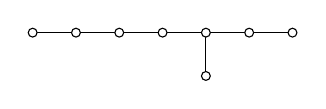
\begin{tikzpicture}[x=.55cm,y=.55cm]
\draw (0,0)--(6,0) (4,0)--(4,-1);
\foreach \x in {0,1,...,6} \draw[fill=white] (\x,0) circle[radius=1.6pt];
\draw[fill=white] (4,-1) circle[radius=1.6pt];
\end{tikzpicture}
\]
\noindent\hangindent=2.8em\hspace*{2.8em}Here each circle denotes a line, and two circles are joined by a line segment whenever the corresponding lines intersect.

\noindent\hspace*{1.2em}\emph{Note.} This singularity has interesting connections with local algebra, invariant theory, and topology.

In case $k=\mathbf C$, Mumford \Goto{bib-mumford-6}{[6]} showed that the completion $\widehat A$ of the ring $A$ at the maximal ideal $\mathfrak m=(x,y,z)$ is also a UFD. This is remarkable, because in general the completion of a local UFD need not be a UFD, although the converse is true (theorem of Mori)---see Samuel \Goto{bib-481-1}{[3]}. Brieskorn \Goto{bib-brieskorn-2}{[2]} showed that the corresponding analytic local ring $\mathbf C\{x,y,z\}/(x^2+y^3+z^5)$ is the \emph{only} nonregular normal $2$-dimensional analytic local ring which is a UFD. Lipman \Goto{bib-479-8}{[2]} generalized this as follows: over any algebraically closed field $k$ of characteristic $\ne2,3,5$, the only nonregular normal complete $2$-dimensional local ring which is a UFD is $k[\![x,y,z]\!]/(x^2+y^3+z^5)$. See also Lipman \Goto{bib-lipman-3}{[3]} for a report on recent work connected with UFD's.

This singularity arose classically out of Klein's work on the icosahedron. The group $I$ of rotations of the icosahedron, which is isomorphic to the simple group of order $60$, acts naturally on the $2$-sphere. Identifying the $2$-sphere with $\mathbf P^1_{\mathbf C}$ by stereographic projection, the group $I$ appears as a finite subgroup of $\operatorname{Aut}\mathbf P^1_{\mathbf C}$. This action lifts to give an action of the binary icosahedral group $\overline I$ on $\mathbf C^2$ by linear transformations of the complex variables $t_1$ and $t_2$. Klein \Goto{bib-klein-2}{[2, I, 2, \S13, p.~62]} found three invariant polynomials $x,y,z$ in $t_1$ and $t_2$, related by the equation $x^2+y^3+z^5=0$. Thus the surface $X$ appears as the quotient of $\mathbf A^2_{\mathbf C}$ by the action of the group $\overline I$. In particular, the local fundamental group of $X$ at $P$ is just $\overline I$.}
% Contents from body/page-435.tex.
\ChapterSheet[10.6]{435}{421}{\Goto{sec-V-6}{6\quad Classification of Surfaces}}{%
With regard to the topology of algebraic varieties over $\mathbf C$, Mumford \Goto{bib-mumford-6}{[6]} showed that a normal algebraic surface over $\mathbf C$, whose underlying topological space (in its \textquotedblleft{}usual\textquotedblright{} topology) is a topological manifold, must be nonsingular. Brieskorn showed that this is not so in higher dimensions. For example, the underlying topological space of the hypersurface in $\mathbf C^4$ defined by $x_1^2+x_2^2+x_3^2+x_4^3=0$ is a manifold. Later Brieskorn \Goto{bib-474-7}{[1]} showed that if one intersects such a singularity with a small sphere around the singular point, then one may get a topological sphere whose differentiable structure is not the standard one. Thus for example, by intersecting the singularity
\[
x_1^2+x_2^2+x_3^2+x_4^3+x_5^{6k-1}=0
\]
in $\mathbf C^5$ with a small sphere around the origin, for $k=1,2,\dots,28$, one obtains all $28$ \EditionText{oriented classes of smooth homotopy $7$-spheres up to diffeomorphism}. See Hirzebruch and Mayer \Goto{bib-477-19-item-1}{[1]} for an account of this work.

\bigskip
\noindent\hypertarget{sec-V-6}{}\BookMark{1}{5.6  Classification of Surfaces}{sec-V-6}\textbf{\large 6\quad Classification of Surfaces}\par\medskip
\noindent In the case of curves, we could achieve a classification as follows. Each birational equivalence class has a unique nonsingular projective model. There is a numerical invariant, the genus $g$, which can take on every value $g\ge0$. For fixed $g$, the curves of genus $g$ are parametrized by the points of the variety of moduli $\mathfrak M_g$ (IV, \S\Goto{sec-IV-5}{5}).

For surfaces, the situation is much more complicated. First of all, the nonsingular projective model is not unique. However, we can standardize by always considering a relatively minimal model. For rational and ruled surfaces, these are known, and for other birational classes there is a unique minimal model (\Goto{result-V-5.8.4}{5.8.4}).

Next, we have the birational invariants $p_a$ (\Goto{result-V-5.6}{5.6}) and $p_g$ (II, \Goto{result-II-8.19}{8.19}), and $K^2$, which is well-defined if we specify the minimal model. However, it is not known exactly which triples of integers can occur as $p_a,p_g,K^2$ of a surface. As to the existence of varieties of moduli, this question is wide open except in some special cases. So we must settle for less complete information than in the case of curves.

In this section we will mention very briefly a few basic results, and refer to Bombieri and Husemoller \Goto{bib-bombieri-husemoller-1}{[1]} and Shafarevich \Goto{bib-482-7}{[1]} for more details and further references.

\medskip
To begin with, for any \EditionText{nonsingular }projective variety $X$ over $k$, we define the \emph{Kodaira dimension} $\kappa(X)$ to be the transcendence degree over $k$ of the ring
\[
R=\bigoplus_{n\ge0}H^0(X,\mathcal L(nK)),
\]
minus $1$, where $K$ is the canonical divisor. One sees, as in the proof of (II, \Goto{result-II-8.19}{8.19}), that $R$ and hence $\kappa$ are birational invariants. Another way of expressing this is that $\kappa$ is the largest dimension of the image of $X$ in $\mathbf P^N$ by the rational map determined by the linear system $|nK|$, for some $n\ge1$, or}
% Contents from body/page-436.tex.
\ChapterSheet[10.6]{436}{422}{\Goto{p-370}{V\quad Surfaces}}{%
\noindent $\kappa=-1$ if $|nK|=\varnothing$ for all $n\ge1$. It is known, for varieties of dimension $n$, that $\kappa$ can take on every value from $-1$ to $n$. For example, for curves, we have $\kappa=-1\Leftrightarrow g=0$; $\kappa=0\Leftrightarrow g=1$; $\kappa=1\Leftrightarrow g\ge2$.

\medskip
We will classify surfaces according to $\kappa=-1,0,1,2$. Some more specific information about each group is provided by the following theorems.

\medskip
\noindent\hypertarget{result-V-6.1}{}\textbf{Theorem 6.1.} \emph{$\kappa=-1\Leftrightarrow|12K|=\varnothing\Leftrightarrow X$ is either rational or ruled.}

\medskip
\noindent\hypertarget{result-V-6.2}{}\textbf{Theorem 6.2} (Castelnuovo). \emph{$X$ is rational $\Leftrightarrow p_a=P_2=0$, where $P_2=\dim H^0(X,\mathcal L(2K))$ is the second plurigenus.}

\smallskip
\noindent\textsc{Proof.} A modern proof over $\mathbf C$, due to Kodaira, is given in Serre \Goto{bib-482-2}{[13]}. In characteristic $p>0$, the proof is due to Zariski \Goto{bib-zariski-5}{[5]}, \Goto{bib-zariski-6}{[6]}, \Goto{bib-483-20}{[9]}.

\medskip
\noindent\hypertarget{result-V-6.2.1}{}\textbf{Remark 6.2.1.} As a consequence of (\Goto{result-V-6.2}{6.2}), one can prove the analogue of L\"uroth's theorem (IV, \Goto{result-IV-2.5.5}{2.5.5}) in dimension $2$: let $k$ be an algebraically closed field, let $L$ be a subfield of a pure transcendental extension $k(t,u)$ of $k$, containing $k$, such that $k(t,u)$ is a finite \emph{separable} extension of $L$. Then $L$ is a pure transcendental extension of $k$. This is Castelnuovo's theorem \textquotedblleft{}on the rationality of plane involutions.\textquotedblright{}

For the proof, let $X'$ be a nonsingular projective model of $L$, and let $X$ be a nonsingular projective model of $k(t,u)$. Then as in (II, \Goto{result-II-8.19}{8.19}) or (II, Ex.~\Goto{ex-II-8.8}{8.8}), using separability, one shows that $p_g(X')\le p_g(X)$ and $P_2(X')\le P_2(X)$, hence $p_g(X')=P_2(X')=0$ since the same is true of $X$. One must also show that $q(X')\le q(X)$ to conclude that $p_a(X')=p_g(X')-q(X')=0$. Then the rationality of \EditionText{$X'$} follows from (\Goto{result-V-6.2}{6.2}). See Serre \Goto{bib-482-2}{[13]} and Zariski \Goto{bib-483-20}{[9]}.

This result is false if one does not assume $k(t,u)$ separable over $L$---see Zariski \Goto{bib-483-20}{[9]} or Shioda \Goto{bib-482-9-item-1}{[1]}.

\medskip
\noindent\hypertarget{result-V-6.3}{}\textbf{Theorem 6.3.} {\itshape \EditionText{On a relatively minimal model, $\kappa=0\Leftrightarrow12K\sim0$. A relatively minimal surface in this class must be one of the following (assume $\operatorname{char}k\ne2,3$):}

\hspace*{1.4em}(1) a K3 surface, which is defined as a surface with $K=0$ and irregularity $q=0$. These have $p_a=p_g=1$;

\hspace*{1.4em}(2) an Enriques surface, which has $p_a=p_g=0$ and $2K=0$;

\hspace*{1.4em}(3) a two-dimensional abelian variety, which has $p_a=-1$, $p_g=1$; or

\hspace*{1.4em}(4) a hyperelliptic surface, which is \EditionText{a quotient $(E\times F)/G$ of elliptic curves by a finite diagonal action, faithful by translations on $E$, with $F/G\cong\mathbf P^1$}.}

\medskip
\noindent\hypertarget{result-V-6.4}{}\textbf{Theorem 6.4.} \emph{A surface with $\kappa=1$ is an elliptic surface, which is a surface $X$ with a morphism $\pi\colon X\to C$ to a curve $C$, such that almost all fibres of $\pi$ are nonsingular elliptic curves (assume $\operatorname{char}k\ne2,3$).}

\medskip
\noindent\hypertarget{result-V-6.5}{}\textbf{Theorem 6.5.} \emph{$\kappa=2$ if and only if for some $n>0$, $|nK|$ determines a birational morphism of $X$ onto its image in $\mathbf P^N$. These are called surfaces of general type.}}
% Contents from body/page-437.tex.
\ChapterSheet{437}{423}{\Goto{sec-V-6}{6\quad Classification of Surfaces}}{%
\noindent\textsc{Exercises}

\smallskip
\noindent\hypertarget{ex-V-6.1}{}\textbf{6.1.} Let $X$ be a surface in $\mathbf P^n$, $n\ge3$, defined as the complete intersection of hypersurfaces of degrees $d_1,\dots,d_{n-2}$, with each $d_i\ge2$. Show that for all but finitely many choices of $(n,d_1,\dots,d_{n-2})$, the surface $X$ is of general type. List the exceptional cases, and where they fit into the classification picture.

\smallskip
\noindent\hypertarget{ex-V-6.2}{}\textbf{6.2.} Prove the following theorem of Chern and Griffiths. Let $X$ be a nonsingular surface of degree $d$ in $\mathbf P^{n+1}_{\mathbf C}$, which is not contained in any hyperplane. If $d<2n$, then $p_g(X)=0$. If $d=2n$, then either $p_g(X)=0$, or $p_g(X)=1$ and $X$ is a K3 surface. [\emph{Hint:} Cut $X$ with a hyperplane and use Clifford's theorem (IV, \Goto{result-IV-5.4}{5.4}). For the last statement, use the Riemann--Roch theorem on $X$ and the Kodaira vanishing theorem (III, \Goto{result-III-7.15}{7.15}).]}
